\documentclass[a4paper,12pt]{article}
\usepackage[margin=1in]{geometry}
\usepackage{array}
\usepackage{longtable}
\usepackage{listings}
\usepackage{xcolor}
\usepackage{graphicx}
\usepackage{tikz}
\usetikzlibrary{calc}
\usepackage{eso-pic}

\AddToShipoutPictureBG{%
  \begin{tikzpicture}[remember picture,overlay]
    \draw[line width=1pt] ($(current page.north west) + (2.2cm,-2.2cm)$) rectangle ($(current page.south east) + (-2.2cm,2.2cm)$);
  \end{tikzpicture}%
}

\begin{document}
\pagestyle{plain}
%% ─── Program 1 ──────────────────────────────────────────────
\noindent\begingroup
\renewcommand{\arraystretch}{1.1}
\begin{longtable}{|p{0.94\textwidth}|}
\hline\endfirsthead\hline\endhead\hline\endfoot\hline\endlastfoot
\rule{0pt}{13pt}Program No: 1 \hfill Date: 29/06/2026 \\
\hline
\rule{0pt}{13pt}Program Title: Create an app that displays name and email id. \\
\hline
\rule{0pt}{13pt}\textbf{MainActivity.java:} \\
\hline
{\ttfamily\small package\ com.example.labcycle;} \\
{\ttfamily\small import\ android.annotation.SuppressLint;} \\
{\ttfamily\small import\ android.os.Bundle;} \\
{\ttfamily\small import\ androidx.activity.EdgeToEdge;} \\
{\ttfamily\small import\ androidx.appcompat.app.AppCompatActivity;} \\
{\ttfamily\small import\ androidx.core.graphics.Insets;} \\
{\ttfamily\small import\ androidx.core.view.ViewCompat;} \\
{\ttfamily\small import\ androidx.core.view.WindowInsetsCompat;} \\
{\ttfamily\small import\ android.view.View;} \\
{\ttfamily\small import\ android.widget.EditText;} \\
{\ttfamily\small import\ android.widget.Button;} \\
{\ttfamily\small import\ android.widget.TextView;} \\
\strut \\
{\ttfamily\small public\ class\ MainActivity\ extends\ AppCompatActivity\ \{} \\
{\ttfamily\small \ \ \ \ EditText\ name,email;} \\
{\ttfamily\small \ \ \ \ Button\ btn;} \\
{\ttfamily\small \ \ \ \ TextView\ t1,t2;} \\
{\ttfamily\small \ \ \ \ @SuppressLint("MissingInflatedId")} \\
{\ttfamily\small \ \ \ \ @Override} \\
{\ttfamily\small \ \ \ \ protected\ void\ onCreate(Bundle\ savedInstanceState)\ \{} \\
{\ttfamily\small \ \ \ \ \ \ \ \ super.onCreate(savedInstanceState);} \\
{\ttfamily\small \ \ \ \ \ \ \ \ EdgeToEdge.enable(this);} \\
{\ttfamily\small \ \ \ \ \ \ \ \ setContentView(R.layout.activity\_main);} \\
{\ttfamily\small \ \ \ \ \ \ \ \ name\ =\ findViewById(R.id.nametxt);} \\
{\ttfamily\small \ \ \ \ \ \ \ \ email\ =\ findViewById(R.id.emailTxt);} \\
{\ttfamily\small \ \ \ \ \ \ \ \ btn\ =\ findViewById(R.id.btnclick);} \\
{\ttfamily\small \ \ \ \ \ \ \ \ t1\ =\ findViewById(R.id.txtView1);} \\
{\ttfamily\small \ \ \ \ \ \ \ \ t2\ =\ findViewById(R.id.txtView2);} \\
{\ttfamily\small \ \ \ \ \ \ \ \ btn.setOnClickListener(new\ View.OnClickListener()\{} \\
{\ttfamily\small \ \ \ \ \ \ \ \ \ \ \ \ @Override} \\
{\ttfamily\small \ \ \ \ \ \ \ \ \ \ \ \ public\ void\ onClick(View\ view)\ \{} \\
{\ttfamily\small \ \ \ \ \ \ \ \ \ \ \ \ \ \ \ \ String\ n1\ =\ name.getText().toString();} \\
{\ttfamily\small \ \ \ \ \ \ \ \ \ \ \ \ \ \ \ \ String\ n2\ =\ email.getText().toString();} \\
{\ttfamily\small \ \ \ \ \ \ \ \ \ \ \ \ \ \ \ \ t1.setText(n1);} \\
{\ttfamily\small \ \ \ \ \ \ \ \ \ \ \ \ \ \ \ \ t2.setText(n2);} \\
{\ttfamily\small \ \ \ \ \ \ \ \ \ \ \ \ \}} \\
{\ttfamily\small \ \ \ \ \ \ \ \ \});} \\
{\ttfamily\small \ \ \ \ \}} \\
{\ttfamily\small \}} \\
\hline
\rule{0pt}{13pt}\textbf{activity\_main.xml:} \\
\hline
{\ttfamily\small \textless{}?xml\ version="1.0"\ encoding="utf-8"?\textgreater{}} \\
{\ttfamily\small \textless{}androidx.constraintlayout.widget.ConstraintLayout} \\
{\ttfamily\small \ \ \ \ xmlns:android="http://schemas.android.com/apk/res/android"} \\
{\ttfamily\small \ \ \ \ xmlns:app="http://schemas.android.com/apk/res-auto"} \\
{\ttfamily\small \ \ \ \ android:layout\_width="match\_parent"} \\
{\ttfamily\small \ \ \ \ android:layout\_height="match\_parent"\textgreater{}} \\
{\ttfamily\small \ \ \ \ \textless{}EditText} \\
{\ttfamily\small \ \ \ \ \ \ \ \ android:id="@+id/nametxt"} \\
{\ttfamily\small \ \ \ \ \ \ \ \ android:layout\_width="250dp"} \\
{\ttfamily\small \ \ \ \ \ \ \ \ android:layout\_height="wrap\_content"} \\
{\ttfamily\small \ \ \ \ \ \ \ \ android:hint="Name"} \\
{\ttfamily\small \ \ \ \ \ \ \ \ app:layout\_constraintTop\_toTopOf="parent"} \\
{\ttfamily\small \ \ \ \ \ \ \ \ app:layout\_constraintStart\_toStartOf="parent"} \\
{\ttfamily\small \ \ \ \ \ \ \ \ app:layout\_constraintEnd\_toEndOf="parent"} \\
{\ttfamily\small \ \ \ \ \ \ \ \ android:layout\_marginTop="150dp"/\textgreater{}} \\
{\ttfamily\small \ \ \ \ \textless{}EditText} \\
{\ttfamily\small \ \ \ \ \ \ \ \ android:id="@+id/emailTxt"} \\
{\ttfamily\small \ \ \ \ \ \ \ \ android:layout\_width="250dp"} \\
{\ttfamily\small \ \ \ \ \ \ \ \ android:layout\_height="wrap\_content"} \\
{\ttfamily\small \ \ \ \ \ \ \ \ android:hint="Email"} \\
{\ttfamily\small \ \ \ \ \ \ \ \ app:layout\_constraintTop\_toBottomOf="@id/nametxt"} \\
{\ttfamily\small \ \ \ \ \ \ \ \ app:layout\_constraintStart\_toStartOf="parent"} \\
{\ttfamily\small \ \ \ \ \ \ \ \ app:layout\_constraintEnd\_toEndOf="parent"} \\
{\ttfamily\small \ \ \ \ \ \ \ \ android:layout\_marginTop="16dp"/\textgreater{}} \\
{\ttfamily\small \ \ \ \ \textless{}Button} \\
{\ttfamily\small \ \ \ \ \ \ \ \ android:id="@+id/btnclick"} \\
{\ttfamily\small \ \ \ \ \ \ \ \ android:layout\_width="wrap\_content"} \\
{\ttfamily\small \ \ \ \ \ \ \ \ android:layout\_height="wrap\_content"} \\
{\ttfamily\small \ \ \ \ \ \ \ \ android:text="Click"} \\
{\ttfamily\small \ \ \ \ \ \ \ \ app:layout\_constraintTop\_toBottomOf="@id/emailTxt"} \\
{\ttfamily\small \ \ \ \ \ \ \ \ app:layout\_constraintStart\_toStartOf="parent"} \\
{\ttfamily\small \ \ \ \ \ \ \ \ app:layout\_constraintEnd\_toEndOf="parent"} \\
{\ttfamily\small \ \ \ \ \ \ \ \ android:layout\_marginTop="20dp"/\textgreater{}} \\
{\ttfamily\small \ \ \ \ \textless{}TextView} \\
{\ttfamily\small \ \ \ \ \ \ \ \ android:id="@+id/txtView1"} \\
{\ttfamily\small \ \ \ \ \ \ \ \ android:layout\_width="wrap\_content"} \\
{\ttfamily\small \ \ \ \ \ \ \ \ android:layout\_height="wrap\_content"} \\
{\ttfamily\small \ \ \ \ \ \ \ \ android:text="Name"} \\
{\ttfamily\small \ \ \ \ \ \ \ \ app:layout\_constraintTop\_toBottomOf="@id/btnclick"} \\
{\ttfamily\small \ \ \ \ \ \ \ \ app:layout\_constraintStart\_toStartOf="parent"} \\
{\ttfamily\small \ \ \ \ \ \ \ \ app:layout\_constraintEnd\_toEndOf="parent"} \\
{\ttfamily\small \ \ \ \ \ \ \ \ android:layout\_marginTop="30dp"/\textgreater{}} \\
{\ttfamily\small \ \ \ \ \textless{}TextView} \\
{\ttfamily\small \ \ \ \ \ \ \ \ android:id="@+id/txtView2"} \\
{\ttfamily\small \ \ \ \ \ \ \ \ android:layout\_width="wrap\_content"} \\
{\ttfamily\small \ \ \ \ \ \ \ \ android:layout\_height="wrap\_content"} \\
{\ttfamily\small \ \ \ \ \ \ \ \ android:text="Email"} \\
{\ttfamily\small \ \ \ \ \ \ \ \ app:layout\_constraintTop\_toBottomOf="@id/txtView1"} \\
{\ttfamily\small \ \ \ \ \ \ \ \ app:layout\_constraintStart\_toStartOf="parent"} \\
{\ttfamily\small \ \ \ \ \ \ \ \ app:layout\_constraintEnd\_toEndOf="parent"} \\
{\ttfamily\small \ \ \ \ \ \ \ \ android:layout\_marginTop="10dp"/\textgreater{}} \\
{\ttfamily\small \textless{}/androidx.constraintlayout.widget.ConstraintLayout\textgreater{}} \\
\hline
Output: \newline \begin{center} 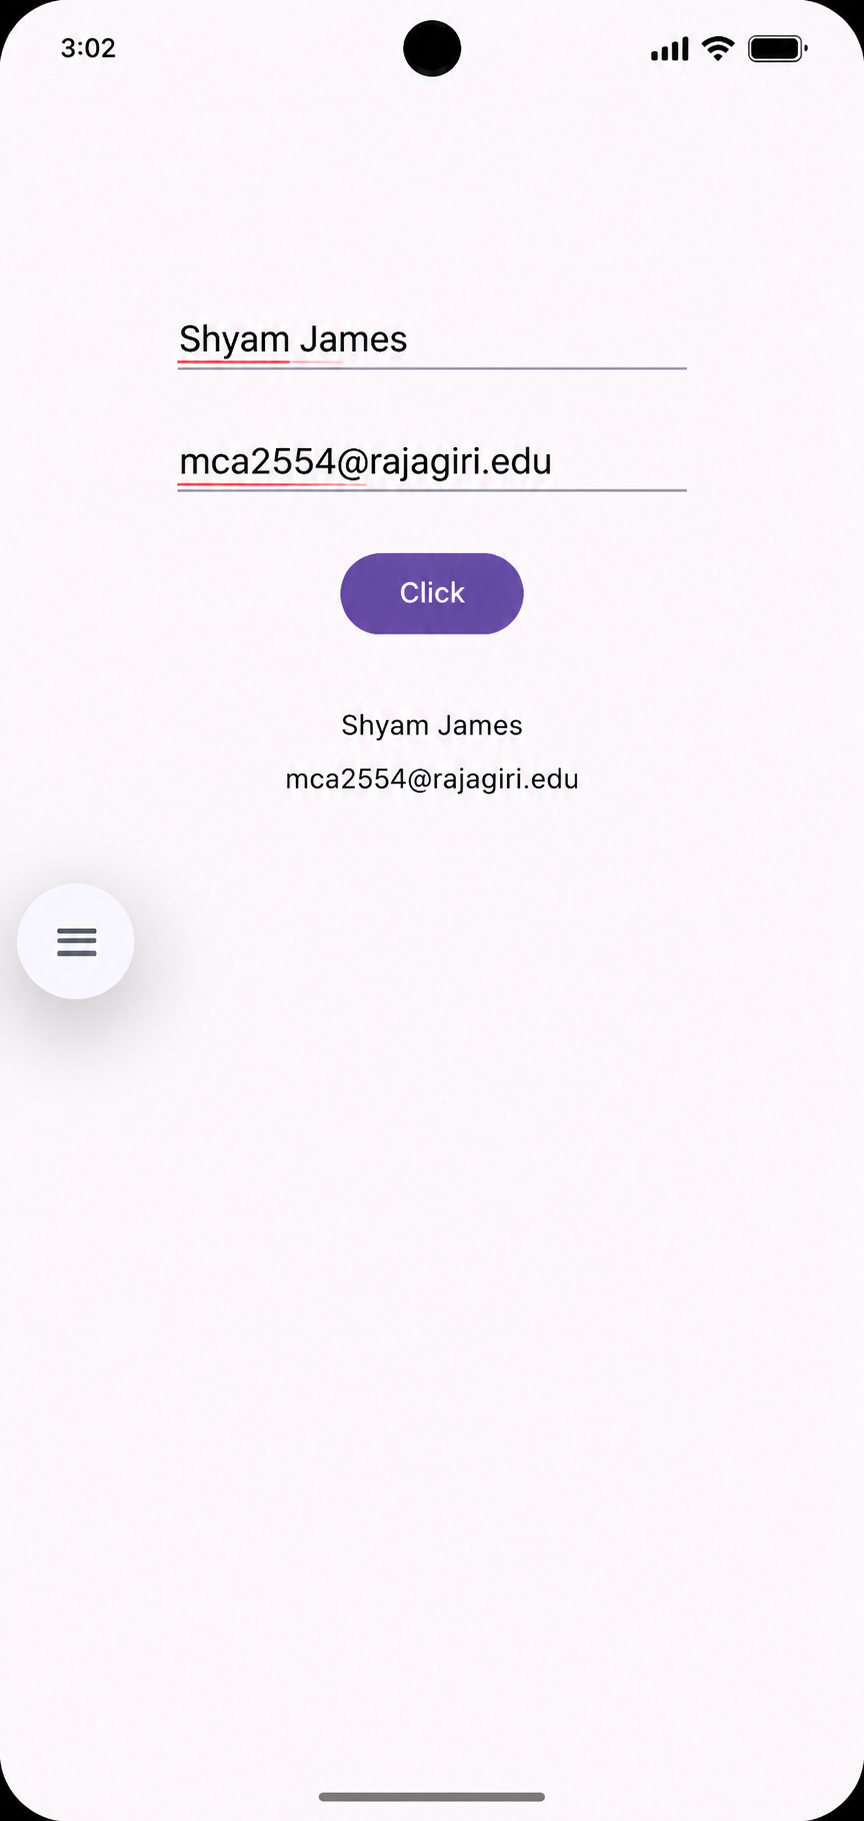
\includegraphics[width=0.45\textwidth]{Output_Screenshots/1.png} \end{center} \\
\end{longtable}
\endgroup

\newpage

%% ─── Program 2 ──────────────────────────────────────────────
\noindent\begingroup
\renewcommand{\arraystretch}{1.1}
\begin{longtable}{|p{0.94\textwidth}|}
\hline\endfirsthead\hline\endhead\hline\endfoot\hline\endlastfoot
\rule{0pt}{13pt}Program No: 2 \hfill Date: 29/06/2026 \\
\hline
\rule{0pt}{13pt}Program Title: Create an app that takes marks of any three subjects from the user and displays its sum and average. \\
\hline
\rule{0pt}{13pt}\textbf{MainActivity.java:} \\
\hline
{\ttfamily\small package\ com.example.labcycle;} \\
\strut \\
{\ttfamily\small import\ android.annotation.SuppressLint;} \\
{\ttfamily\small import\ android.os.Bundle;} \\
{\ttfamily\small import\ androidx.activity.EdgeToEdge;} \\
{\ttfamily\small import\ androidx.appcompat.app.AppCompatActivity;} \\
{\ttfamily\small import\ androidx.core.graphics.Insets;} \\
{\ttfamily\small import\ androidx.core.view.ViewCompat;} \\
{\ttfamily\small import\ androidx.core.view.WindowInsetsCompat;} \\
{\ttfamily\small import\ android.view.View;} \\
{\ttfamily\small import\ android.widget.EditText;} \\
{\ttfamily\small import\ android.widget.Button;} \\
{\ttfamily\small import\ android.widget.TextView;} \\
\strut \\
{\ttfamily\small public\ class\ MainActivity\ extends\ AppCompatActivity\ \{} \\
{\ttfamily\small \ \ \ \ EditText\ m1,\ m2,\ m3;} \\
{\ttfamily\small \ \ \ \ Button\ btn;} \\
{\ttfamily\small \ \ \ \ TextView\ t1,\ t2;} \\
\strut \\
{\ttfamily\small \ \ \ \ @SuppressLint("MissingInflatedId")} \\
{\ttfamily\small \ \ \ \ @Override} \\
{\ttfamily\small \ \ \ \ protected\ void\ onCreate(Bundle\ savedInstanceState)\ \{} \\
{\ttfamily\small \ \ \ \ \ \ \ \ super.onCreate(savedInstanceState);} \\
{\ttfamily\small \ \ \ \ \ \ \ \ EdgeToEdge.enable(this);} \\
{\ttfamily\small \ \ \ \ \ \ \ \ setContentView(R.layout.activity\_main);} \\
\strut \\
{\ttfamily\small \ \ \ \ \ \ \ \ m1\ =\ findViewById(R.id.mark1);} \\
{\ttfamily\small \ \ \ \ \ \ \ \ m2\ =\ findViewById(R.id.mark2);} \\
{\ttfamily\small \ \ \ \ \ \ \ \ m3\ =\ findViewById(R.id.mark3);} \\
{\ttfamily\small \ \ \ \ \ \ \ \ btn\ =\ findViewById(R.id.btncal);} \\
{\ttfamily\small \ \ \ \ \ \ \ \ t1\ =\ findViewById(R.id.textView4);} \\
{\ttfamily\small \ \ \ \ \ \ \ \ t2\ =\ findViewById(R.id.textView5);} \\
\strut \\
{\ttfamily\small \ \ \ \ \ \ \ \ btn.setOnClickListener(new\ View.OnClickListener()\ \{} \\
{\ttfamily\small \ \ \ \ \ \ \ \ \ \ \ \ @Override} \\
{\ttfamily\small \ \ \ \ \ \ \ \ \ \ \ \ public\ void\ onClick(View\ view)\ \{} \\
{\ttfamily\small \ \ \ \ \ \ \ \ \ \ \ \ \ \ \ \ int\ n1\ =\ Integer.parseInt(m1.getText().toString());} \\
{\ttfamily\small \ \ \ \ \ \ \ \ \ \ \ \ \ \ \ \ int\ n2\ =\ Integer.parseInt(m2.getText().toString());} \\
{\ttfamily\small \ \ \ \ \ \ \ \ \ \ \ \ \ \ \ \ int\ n3\ =\ Integer.parseInt(m3.getText().toString());} \\
{\ttfamily\small \ \ \ \ \ \ \ \ \ \ \ \ \ \ \ \ int\ sums\ =\ n1\ +\ n2\ +\ n3;} \\
{\ttfamily\small \ \ \ \ \ \ \ \ \ \ \ \ \ \ \ \ int\ avg\ =\ sums\ /\ 3;} \\
{\ttfamily\small \ \ \ \ \ \ \ \ \ \ \ \ \ \ \ \ t1.setText("Sum\ is\ "\ +\ sums);} \\
{\ttfamily\small \ \ \ \ \ \ \ \ \ \ \ \ \ \ \ \ t2.setText("Average\ is\ "\ +\ avg);} \\
{\ttfamily\small \ \ \ \ \ \ \ \ \ \ \ \ \}} \\
{\ttfamily\small \ \ \ \ \ \ \ \ \});} \\
{\ttfamily\small \ \ \ \ \}} \\
{\ttfamily\small \}} \\
\hline
\rule{0pt}{13pt}\textbf{activity\_main.xml:} \\
\hline
{\ttfamily\small \textless{}?xml\ version="1.0"\ encoding="utf-8"?\textgreater{}} \\
{\ttfamily\small \textless{}androidx.constraintlayout.widget.ConstraintLayout} \\
{\ttfamily\small \ \ \ \ xmlns:android="http://schemas.android.com/apk/res/android"} \\
{\ttfamily\small \ \ \ \ xmlns:app="http://schemas.android.com/apk/res-auto"} \\
{\ttfamily\small \ \ \ \ xmlns:tools="http://schemas.android.com/tools"} \\
{\ttfamily\small \ \ \ \ android:layout\_width="match\_parent"} \\
{\ttfamily\small \ \ \ \ android:layout\_height="match\_parent"\textgreater{}} \\
\strut \\
{\ttfamily\small \ \ \ \ \textless{}EditText} \\
{\ttfamily\small \ \ \ \ \ \ \ \ android:id="@+id/mark1"} \\
{\ttfamily\small \ \ \ \ \ \ \ \ android:layout\_width="wrap\_content"} \\
{\ttfamily\small \ \ \ \ \ \ \ \ android:layout\_height="wrap\_content"} \\
{\ttfamily\small \ \ \ \ \ \ \ \ android:layout\_marginEnd="92dp"} \\
{\ttfamily\small \ \ \ \ \ \ \ \ android:layout\_marginBottom="43dp"} \\
{\ttfamily\small \ \ \ \ \ \ \ \ android:ems="10"} \\
{\ttfamily\small \ \ \ \ \ \ \ \ android:inputType="number"} \\
{\ttfamily\small \ \ \ \ \ \ \ \ android:text="mark1"} \\
{\ttfamily\small \ \ \ \ \ \ \ \ app:layout\_constraintBottom\_toTopOf="@+id/mark2"} \\
{\ttfamily\small \ \ \ \ \ \ \ \ app:layout\_constraintEnd\_toEndOf="parent"\ /\textgreater{}} \\
\strut \\
{\ttfamily\small \ \ \ \ \textless{}EditText} \\
{\ttfamily\small \ \ \ \ \ \ \ \ android:id="@+id/mark2"} \\
{\ttfamily\small \ \ \ \ \ \ \ \ android:layout\_width="wrap\_content"} \\
{\ttfamily\small \ \ \ \ \ \ \ \ android:layout\_height="wrap\_content"} \\
{\ttfamily\small \ \ \ \ \ \ \ \ android:layout\_marginEnd="91dp"} \\
{\ttfamily\small \ \ \ \ \ \ \ \ android:layout\_marginBottom="40dp"} \\
{\ttfamily\small \ \ \ \ \ \ \ \ android:ems="10"} \\
{\ttfamily\small \ \ \ \ \ \ \ \ android:inputType="number"} \\
{\ttfamily\small \ \ \ \ \ \ \ \ android:text="mark2"} \\
{\ttfamily\small \ \ \ \ \ \ \ \ app:layout\_constraintBottom\_toTopOf="@+id/mark3"} \\
{\ttfamily\small \ \ \ \ \ \ \ \ app:layout\_constraintEnd\_toEndOf="parent"\ /\textgreater{}} \\
\strut \\
{\ttfamily\small \ \ \ \ \textless{}EditText} \\
{\ttfamily\small \ \ \ \ \ \ \ \ android:id="@+id/mark3"} \\
{\ttfamily\small \ \ \ \ \ \ \ \ android:layout\_width="wrap\_content"} \\
{\ttfamily\small \ \ \ \ \ \ \ \ android:layout\_height="wrap\_content"} \\
{\ttfamily\small \ \ \ \ \ \ \ \ android:layout\_marginEnd="85dp"} \\
{\ttfamily\small \ \ \ \ \ \ \ \ android:layout\_marginBottom="48dp"} \\
{\ttfamily\small \ \ \ \ \ \ \ \ android:ems="10"} \\
{\ttfamily\small \ \ \ \ \ \ \ \ android:inputType="numberSigned"} \\
{\ttfamily\small \ \ \ \ \ \ \ \ android:text="mark3"} \\
{\ttfamily\small \ \ \ \ \ \ \ \ app:layout\_constraintBottom\_toTopOf="@+id/btncal"} \\
{\ttfamily\small \ \ \ \ \ \ \ \ app:layout\_constraintEnd\_toEndOf="parent"\ /\textgreater{}} \\
\strut \\
{\ttfamily\small \ \ \ \ \textless{}Button} \\
{\ttfamily\small \ \ \ \ \ \ \ \ android:id="@+id/btncal"} \\
{\ttfamily\small \ \ \ \ \ \ \ \ android:layout\_width="wrap\_content"} \\
{\ttfamily\small \ \ \ \ \ \ \ \ android:layout\_height="wrap\_content"} \\
{\ttfamily\small \ \ \ \ \ \ \ \ android:layout\_marginEnd="182dp"} \\
{\ttfamily\small \ \ \ \ \ \ \ \ android:layout\_marginBottom="49dp"} \\
{\ttfamily\small \ \ \ \ \ \ \ \ android:text="Button"} \\
{\ttfamily\small \ \ \ \ \ \ \ \ app:layout\_constraintBottom\_toTopOf="@+id/textView4"} \\
{\ttfamily\small \ \ \ \ \ \ \ \ app:layout\_constraintEnd\_toEndOf="parent"\ /\textgreater{}} \\
\strut \\
{\ttfamily\small \ \ \ \ \textless{}TextView} \\
{\ttfamily\small \ \ \ \ \ \ \ \ android:id="@+id/textView4"} \\
{\ttfamily\small \ \ \ \ \ \ \ \ android:layout\_width="wrap\_content"} \\
{\ttfamily\small \ \ \ \ \ \ \ \ android:layout\_height="wrap\_content"} \\
{\ttfamily\small \ \ \ \ \ \ \ \ android:layout\_marginEnd="202dp"} \\
{\ttfamily\small \ \ \ \ \ \ \ \ android:layout\_marginBottom="160dp"} \\
{\ttfamily\small \ \ \ \ \ \ \ \ android:text="TextView"} \\
{\ttfamily\small \ \ \ \ \ \ \ \ app:layout\_constraintBottom\_toBottomOf="parent"} \\
{\ttfamily\small \ \ \ \ \ \ \ \ app:layout\_constraintEnd\_toEndOf="parent"\ /\textgreater{}} \\
\strut \\
{\ttfamily\small \ \ \ \ \textless{}TextView} \\
{\ttfamily\small \ \ \ \ \ \ \ \ android:id="@+id/textView5"} \\
{\ttfamily\small \ \ \ \ \ \ \ \ android:layout\_width="wrap\_content"} \\
{\ttfamily\small \ \ \ \ \ \ \ \ android:layout\_height="wrap\_content"} \\
{\ttfamily\small \ \ \ \ \ \ \ \ android:layout\_marginEnd="200dp"} \\
{\ttfamily\small \ \ \ \ \ \ \ \ android:layout\_marginBottom="120dp"} \\
{\ttfamily\small \ \ \ \ \ \ \ \ android:text="TextView"} \\
{\ttfamily\small \ \ \ \ \ \ \ \ app:layout\_constraintBottom\_toBottomOf="parent"} \\
{\ttfamily\small \ \ \ \ \ \ \ \ app:layout\_constraintEnd\_toEndOf="parent"\ /\textgreater{}} \\
\strut \\
{\ttfamily\small \textless{}/androidx.constraintlayout.widget.ConstraintLayout\textgreater{}} \\
\hline
Output: \newline \begin{center} 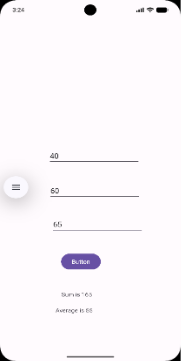
\includegraphics[width=0.45\textwidth]{Output_Screenshots/2.png} \end{center} \\
\end{longtable}
\endgroup

\newpage

%% ─── Program 3 ──────────────────────────────────────────────
\noindent\begingroup
\renewcommand{\arraystretch}{1.1}
\begin{longtable}{|p{0.94\textwidth}|}
\hline\endfirsthead\hline\endhead\hline\endfoot\hline\endlastfoot
\rule{0pt}{13pt}Program No: 3 \hfill Date: 29/06/2026 \\
\hline
\rule{0pt}{13pt}Program Title: Create suitable apps to design the different layouts of the androidstudio. \\
\hline
\rule{0pt}{13pt}\textbf{MainActivity.java:} \\
\hline
{\ttfamily\small package\ com.example.labcycle;} \\
\strut \\
{\ttfamily\small import\ android.os.Bundle;} \\
{\ttfamily\small import\ android.widget.Button;} \\
{\ttfamily\small import\ android.widget.Toast;} \\
{\ttfamily\small import\ androidx.appcompat.app.AppCompatActivity;} \\
\strut \\
{\ttfamily\small public\ class\ MainActivity\ extends\ AppCompatActivity\ \{} \\
{\ttfamily\small \ \ \ \ Button\ button1,\ button2,\ button3;} \\
\strut \\
{\ttfamily\small \ \ \ \ @Override} \\
{\ttfamily\small \ \ \ \ protected\ void\ onCreate(Bundle\ savedInstanceState)\ \{} \\
{\ttfamily\small \ \ \ \ \ \ \ \ super.onCreate(savedInstanceState);} \\
{\ttfamily\small \ \ \ \ \ \ \ \ setContentView(R.layout.activity\_main);} \\
\strut \\
{\ttfamily\small \ \ \ \ \ \ \ \ button1\ =\ findViewById(R.id.button1);} \\
{\ttfamily\small \ \ \ \ \ \ \ \ button2\ =\ findViewById(R.id.button2);} \\
{\ttfamily\small \ \ \ \ \ \ \ \ button3\ =\ findViewById(R.id.button3);} \\
\strut \\
{\ttfamily\small \ \ \ \ \ \ \ \ button1.setOnClickListener(v\ -\textgreater{}} \\
{\ttfamily\small \ \ \ \ \ \ \ \ \ \ \ \ \ \ \ \ Toast.makeText(this,\ "LinearLayout\ Button\ 1",\ Toast.LENGTH\_SHORT).show());} \\
{\ttfamily\small \ \ \ \ \ \ \ \ button2.setOnClickListener(v\ -\textgreater{}} \\
{\ttfamily\small \ \ \ \ \ \ \ \ \ \ \ \ \ \ \ \ Toast.makeText(this,\ "LinearLayout\ Button\ 2",\ Toast.LENGTH\_SHORT).show());} \\
{\ttfamily\small \ \ \ \ \ \ \ \ button3.setOnClickListener(v\ -\textgreater{}} \\
{\ttfamily\small \ \ \ \ \ \ \ \ \ \ \ \ \ \ \ \ Toast.makeText(this,\ "RelativeLayout\ Button",\ Toast.LENGTH\_SHORT).show());} \\
{\ttfamily\small \ \ \ \ \}} \\
{\ttfamily\small \}} \\
\hline
\rule{0pt}{13pt}\textbf{activity\_main.xml:} \\
\hline
{\ttfamily\small \textless{}?xml\ version="1.0"\ encoding="utf-8"?\textgreater{}} \\
{\ttfamily\small \textless{}ScrollView\ xmlns:android="http://schemas.android.com/apk/res/android"} \\
{\ttfamily\small \ \ \ \ android:layout\_width="match\_parent"} \\
{\ttfamily\small \ \ \ \ android:layout\_height="match\_parent"\textgreater{}} \\
\strut \\
{\ttfamily\small \ \ \ \ \textless{}LinearLayout} \\
{\ttfamily\small \ \ \ \ \ \ \ \ android:layout\_width="match\_parent"} \\
{\ttfamily\small \ \ \ \ \ \ \ \ android:layout\_height="wrap\_content"} \\
{\ttfamily\small \ \ \ \ \ \ \ \ android:orientation="vertical"} \\
{\ttfamily\small \ \ \ \ \ \ \ \ android:padding="16dp"\textgreater{}} \\
\strut \\
{\ttfamily\small \ \ \ \ \ \ \ \ \textless{}!--\ LinearLayout\ --\textgreater{}} \\
{\ttfamily\small \ \ \ \ \ \ \ \ \textless{}TextView} \\
{\ttfamily\small \ \ \ \ \ \ \ \ \ \ \ \ android:layout\_width="wrap\_content"} \\
{\ttfamily\small \ \ \ \ \ \ \ \ \ \ \ \ android:layout\_height="wrap\_content"} \\
{\ttfamily\small \ \ \ \ \ \ \ \ \ \ \ \ android:text="Linear\ Layout"} \\
{\ttfamily\small \ \ \ \ \ \ \ \ \ \ \ \ android:textStyle="bold"} \\
{\ttfamily\small \ \ \ \ \ \ \ \ \ \ \ \ android:textSize="18sp"/\textgreater{}} \\
\strut \\
{\ttfamily\small \ \ \ \ \ \ \ \ \textless{}LinearLayout} \\
{\ttfamily\small \ \ \ \ \ \ \ \ \ \ \ \ android:layout\_width="match\_parent"} \\
{\ttfamily\small \ \ \ \ \ \ \ \ \ \ \ \ android:layout\_height="wrap\_content"} \\
{\ttfamily\small \ \ \ \ \ \ \ \ \ \ \ \ android:orientation="horizontal"} \\
{\ttfamily\small \ \ \ \ \ \ \ \ \ \ \ \ android:layout\_marginBottom="20dp"\textgreater{}} \\
\strut \\
{\ttfamily\small \ \ \ \ \ \ \ \ \ \ \ \ \textless{}Button} \\
{\ttfamily\small \ \ \ \ \ \ \ \ \ \ \ \ \ \ \ \ android:id="@+id/button1"} \\
{\ttfamily\small \ \ \ \ \ \ \ \ \ \ \ \ \ \ \ \ android:layout\_width="0dp"} \\
{\ttfamily\small \ \ \ \ \ \ \ \ \ \ \ \ \ \ \ \ android:layout\_height="wrap\_content"} \\
{\ttfamily\small \ \ \ \ \ \ \ \ \ \ \ \ \ \ \ \ android:layout\_weight="1"} \\
{\ttfamily\small \ \ \ \ \ \ \ \ \ \ \ \ \ \ \ \ android:text="Button\ 1"/\textgreater{}} \\
\strut \\
{\ttfamily\small \ \ \ \ \ \ \ \ \ \ \ \ \textless{}Button} \\
{\ttfamily\small \ \ \ \ \ \ \ \ \ \ \ \ \ \ \ \ android:id="@+id/button2"} \\
{\ttfamily\small \ \ \ \ \ \ \ \ \ \ \ \ \ \ \ \ android:layout\_width="0dp"} \\
{\ttfamily\small \ \ \ \ \ \ \ \ \ \ \ \ \ \ \ \ android:layout\_height="wrap\_content"} \\
{\ttfamily\small \ \ \ \ \ \ \ \ \ \ \ \ \ \ \ \ android:layout\_weight="1"} \\
{\ttfamily\small \ \ \ \ \ \ \ \ \ \ \ \ \ \ \ \ android:text="Button\ 2"/\textgreater{}} \\
{\ttfamily\small \ \ \ \ \ \ \ \ \textless{}/LinearLayout\textgreater{}} \\
\strut \\
{\ttfamily\small \ \ \ \ \ \ \ \ \textless{}!--\ RelativeLayout\ --\textgreater{}} \\
{\ttfamily\small \ \ \ \ \ \ \ \ \textless{}TextView} \\
{\ttfamily\small \ \ \ \ \ \ \ \ \ \ \ \ android:layout\_width="wrap\_content"} \\
{\ttfamily\small \ \ \ \ \ \ \ \ \ \ \ \ android:layout\_height="wrap\_content"} \\
{\ttfamily\small \ \ \ \ \ \ \ \ \ \ \ \ android:text="Relative\ Layout"} \\
{\ttfamily\small \ \ \ \ \ \ \ \ \ \ \ \ android:textStyle="bold"} \\
{\ttfamily\small \ \ \ \ \ \ \ \ \ \ \ \ android:textSize="18sp"/\textgreater{}} \\
\strut \\
{\ttfamily\small \ \ \ \ \ \ \ \ \textless{}RelativeLayout} \\
{\ttfamily\small \ \ \ \ \ \ \ \ \ \ \ \ android:layout\_width="match\_parent"} \\
{\ttfamily\small \ \ \ \ \ \ \ \ \ \ \ \ android:layout\_height="120dp"} \\
{\ttfamily\small \ \ \ \ \ \ \ \ \ \ \ \ android:background="\#DDDDDD"} \\
{\ttfamily\small \ \ \ \ \ \ \ \ \ \ \ \ android:layout\_marginBottom="20dp"\textgreater{}} \\
\strut \\
{\ttfamily\small \ \ \ \ \ \ \ \ \ \ \ \ \textless{}TextView} \\
{\ttfamily\small \ \ \ \ \ \ \ \ \ \ \ \ \ \ \ \ android:id="@+id/text1"} \\
{\ttfamily\small \ \ \ \ \ \ \ \ \ \ \ \ \ \ \ \ android:layout\_width="wrap\_content"} \\
{\ttfamily\small \ \ \ \ \ \ \ \ \ \ \ \ \ \ \ \ android:layout\_height="wrap\_content"} \\
{\ttfamily\small \ \ \ \ \ \ \ \ \ \ \ \ \ \ \ \ android:text="Top\ Left"/\textgreater{}} \\
\strut \\
{\ttfamily\small \ \ \ \ \ \ \ \ \ \ \ \ \textless{}Button} \\
{\ttfamily\small \ \ \ \ \ \ \ \ \ \ \ \ \ \ \ \ android:id="@+id/button3"} \\
{\ttfamily\small \ \ \ \ \ \ \ \ \ \ \ \ \ \ \ \ android:layout\_width="wrap\_content"} \\
{\ttfamily\small \ \ \ \ \ \ \ \ \ \ \ \ \ \ \ \ android:layout\_height="wrap\_content"} \\
{\ttfamily\small \ \ \ \ \ \ \ \ \ \ \ \ \ \ \ \ android:text="Bottom\ Right"} \\
{\ttfamily\small \ \ \ \ \ \ \ \ \ \ \ \ \ \ \ \ android:layout\_alignParentBottom="true"} \\
{\ttfamily\small \ \ \ \ \ \ \ \ \ \ \ \ \ \ \ \ android:layout\_alignParentEnd="true"/\textgreater{}} \\
{\ttfamily\small \ \ \ \ \ \ \ \ \textless{}/RelativeLayout\textgreater{}} \\
\strut \\
{\ttfamily\small \ \ \ \ \ \ \ \ \textless{}!--\ FrameLayout\ --\textgreater{}} \\
{\ttfamily\small \ \ \ \ \ \ \ \ \textless{}TextView} \\
{\ttfamily\small \ \ \ \ \ \ \ \ \ \ \ \ android:layout\_width="wrap\_content"} \\
{\ttfamily\small \ \ \ \ \ \ \ \ \ \ \ \ android:layout\_height="wrap\_content"} \\
{\ttfamily\small \ \ \ \ \ \ \ \ \ \ \ \ android:text="Frame\ Layout"} \\
{\ttfamily\small \ \ \ \ \ \ \ \ \ \ \ \ android:textStyle="bold"} \\
{\ttfamily\small \ \ \ \ \ \ \ \ \ \ \ \ android:textSize="18sp"/\textgreater{}} \\
\strut \\
{\ttfamily\small \ \ \ \ \ \ \ \ \textless{}FrameLayout} \\
{\ttfamily\small \ \ \ \ \ \ \ \ \ \ \ \ android:layout\_width="match\_parent"} \\
{\ttfamily\small \ \ \ \ \ \ \ \ \ \ \ \ android:layout\_height="150dp"} \\
{\ttfamily\small \ \ \ \ \ \ \ \ \ \ \ \ android:background="\#2196F3"\textgreater{}} \\
\strut \\
{\ttfamily\small \ \ \ \ \ \ \ \ \ \ \ \ \textless{}TextView} \\
{\ttfamily\small \ \ \ \ \ \ \ \ \ \ \ \ \ \ \ \ android:layout\_width="wrap\_content"} \\
{\ttfamily\small \ \ \ \ \ \ \ \ \ \ \ \ \ \ \ \ android:layout\_height="wrap\_content"} \\
{\ttfamily\small \ \ \ \ \ \ \ \ \ \ \ \ \ \ \ \ android:text="FrameLayout\ Example"} \\
{\ttfamily\small \ \ \ \ \ \ \ \ \ \ \ \ \ \ \ \ android:textColor="\#FFFFFF"} \\
{\ttfamily\small \ \ \ \ \ \ \ \ \ \ \ \ \ \ \ \ android:layout\_gravity="center"/\textgreater{}} \\
{\ttfamily\small \ \ \ \ \ \ \ \ \textless{}/FrameLayout\textgreater{}} \\
{\ttfamily\small \ \ \ \ \textless{}/LinearLayout\textgreater{}} \\
{\ttfamily\small \textless{}/ScrollView\textgreater{}} \\
\hline
Output: \newline \begin{center} 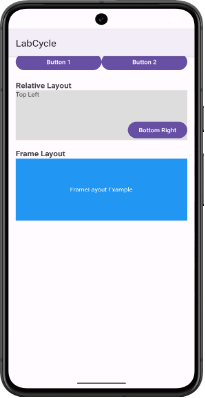
\includegraphics[width=0.45\textwidth]{Output_Screenshots/3.png} \end{center} \\
\end{longtable}
\endgroup

\newpage

%% ─── Program 4 ──────────────────────────────────────────────
\noindent\begingroup
\renewcommand{\arraystretch}{1.1}
\begin{longtable}{|p{0.94\textwidth}|}
\hline\endfirsthead\hline\endhead\hline\endfoot\hline\endlastfoot
\rule{0pt}{13pt}Program No: 4 \hfill Date: 29/06/2026 \\
\hline
\rule{0pt}{13pt}Program Title: Develop a simple calculator app. \\
\hline
\rule{0pt}{13pt}\textbf{MainActivity.java:} \\
\hline
{\ttfamily\small package\ com.example.pg04\_calculator;} \\
\strut \\
{\ttfamily\small import\ android.os.Bundle;} \\
\strut \\
{\ttfamily\small import\ androidx.activity.EdgeToEdge;} \\
{\ttfamily\small import\ androidx.appcompat.app.AppCompatActivity;} \\
{\ttfamily\small import\ androidx.core.graphics.Insets;} \\
{\ttfamily\small import\ androidx.core.view.ViewCompat;} \\
{\ttfamily\small import\ androidx.core.view.WindowInsetsCompat;} \\
{\ttfamily\small import\ android.widget.TextView;} \\
{\ttfamily\small import\ android.widget.Button;} \\
{\ttfamily\small import\ android.widget.EditText;} \\
\strut \\
{\ttfamily\small public\ class\ MainActivity\ extends\ AppCompatActivity\ \{} \\
{\ttfamily\small \ \ \ \ TextView\ result;} \\
{\ttfamily\small \ \ \ \ Button\ ad,\ sub,\ div,\ mult;} \\
{\ttfamily\small \ \ \ \ EditText\ no1,\ no2;} \\
{\ttfamily\small \ \ \ \ @Override} \\
{\ttfamily\small \ \ \ \ protected\ void\ onCreate(Bundle\ savedInstanceState)\ \{} \\
{\ttfamily\small \ \ \ \ \ \ \ \ super.onCreate(savedInstanceState);} \\
{\ttfamily\small \ \ \ \ \ \ \ \ EdgeToEdge.enable(this);} \\
{\ttfamily\small \ \ \ \ \ \ \ \ setContentView(R.layout.activity\_main);} \\
{\ttfamily\small \ \ \ \ \ \ \ \ result\ =\ findViewById(R.id.result);} \\
{\ttfamily\small \ \ \ \ \ \ \ \ ad\ =\ findViewById(R.id.ad);} \\
{\ttfamily\small \ \ \ \ \ \ \ \ sub\ =\ findViewById(R.id.sub);} \\
{\ttfamily\small \ \ \ \ \ \ \ \ div\ =\ findViewById(R.id.div);} \\
{\ttfamily\small \ \ \ \ \ \ \ \ mult\ =findViewById(R.id.mult);} \\
{\ttfamily\small \ \ \ \ \ \ \ \ no1\ =\ findViewById(R.id.no1);} \\
{\ttfamily\small \ \ \ \ \ \ \ \ no2\ =\ findViewById(R.id.no2);} \\
\strut \\
{\ttfamily\small \ \ \ \ \ \ \ \ ad.setOnClickListener(v\ -\textgreater{}\ \{} \\
{\ttfamily\small \ \ \ \ \ \ \ \ \ \ \ \ int\ a\ =\ Integer.parseInt(no1.getText().toString());} \\
{\ttfamily\small \ \ \ \ \ \ \ \ \ \ \ \ int\ b\ =\ Integer.parseInt(no2.getText().toString());} \\
{\ttfamily\small \ \ \ \ \ \ \ \ \ \ \ \ int\ res\ =\ a\ +\ b;} \\
{\ttfamily\small \ \ \ \ \ \ \ \ \ \ \ \ result.setText(res+"");} \\
{\ttfamily\small \ \ \ \ \ \ \ \ \});} \\
\strut \\
{\ttfamily\small \ \ \ \ \ \ \ \ sub.setOnClickListener(v\ -\textgreater{}\ \{} \\
{\ttfamily\small \ \ \ \ \ \ \ \ \ \ \ \ int\ a\ =\ Integer.parseInt(no1.getText().toString());} \\
{\ttfamily\small \ \ \ \ \ \ \ \ \ \ \ \ int\ b\ =\ Integer.parseInt(no2.getText().toString());} \\
{\ttfamily\small \ \ \ \ \ \ \ \ \ \ \ \ int\ res\ =\ a\ -\ b;} \\
{\ttfamily\small \ \ \ \ \ \ \ \ \ \ \ \ result.setText(res+"");} \\
{\ttfamily\small \ \ \ \ \ \ \ \ \});} \\
\strut \\
{\ttfamily\small \ \ \ \ \ \ \ \ mult.setOnClickListener(v\ -\textgreater{}\ \{} \\
{\ttfamily\small \ \ \ \ \ \ \ \ \ \ \ \ int\ a\ =\ Integer.parseInt(no1.getText().toString());} \\
{\ttfamily\small \ \ \ \ \ \ \ \ \ \ \ \ int\ b\ =\ Integer.parseInt(no2.getText().toString());} \\
{\ttfamily\small \ \ \ \ \ \ \ \ \ \ \ \ int\ res\ =\ a\ *\ b;} \\
{\ttfamily\small \ \ \ \ \ \ \ \ \ \ \ \ result.setText(res+"");} \\
\strut \\
{\ttfamily\small \ \ \ \ \ \ \ \ \});} \\
\strut \\
{\ttfamily\small \ \ \ \ \ \ \ \ div.setOnClickListener(v\ -\textgreater{}\ \{} \\
{\ttfamily\small \ \ \ \ \ \ \ \ \ \ \ \ int\ a\ =\ Integer.parseInt(no1.getText().toString());} \\
{\ttfamily\small \ \ \ \ \ \ \ \ \ \ \ \ int\ b\ =\ Integer.parseInt(no2.getText().toString());} \\
{\ttfamily\small \ \ \ \ \ \ \ \ \ \ \ \ if(b!=0)\ \{} \\
{\ttfamily\small \ \ \ \ \ \ \ \ \ \ \ \ \ \ \ \ int\ res\ =\ a\ /\ b;} \\
{\ttfamily\small \ \ \ \ \ \ \ \ \ \ \ \ \ \ \ \ result.setText(res+"");} \\
{\ttfamily\small \ \ \ \ \ \ \ \ \ \ \ \ \}} \\
{\ttfamily\small \ \ \ \ \ \ \ \ \ \ \ \ else} \\
{\ttfamily\small \ \ \ \ \ \ \ \ \ \ \ \ \ \ \ \ result.setText("Error:\ Divsion\ /\ 0");} \\
{\ttfamily\small \ \ \ \ \ \ \ \ \});} \\
{\ttfamily\small \ \ \ \ \}} \\
{\ttfamily\small \}} \\
\hline
\rule{0pt}{13pt}\textbf{activity\_main.xml:} \\
\hline
{\ttfamily\small \textless{}?xml\ version="1.0"\ encoding="utf-8"?\textgreater{}} \\
{\ttfamily\small \textless{}androidx.constraintlayout.widget.ConstraintLayout\ xmlns:android="http://schemas.android.com/apk/res/android"} \\
{\ttfamily\small \ \ \ \ xmlns:app="http://schemas.android.com/apk/res-auto"} \\
{\ttfamily\small \ \ \ \ xmlns:tools="http://schemas.android.com/tools"} \\
{\ttfamily\small \ \ \ \ android:id="@+id/main"} \\
{\ttfamily\small \ \ \ \ android:layout\_width="match\_parent"} \\
{\ttfamily\small \ \ \ \ android:layout\_height="match\_parent"} \\
{\ttfamily\small \ \ \ \ tools:context=".MainActivity"\textgreater{}} \\
\strut \\
{\ttfamily\small \ \ \ \ \textless{}TextView} \\
{\ttfamily\small \ \ \ \ \ \ \ \ android:layout\_width="wrap\_content"} \\
{\ttfamily\small \ \ \ \ \ \ \ \ android:layout\_height="wrap\_content"} \\
{\ttfamily\small \ \ \ \ \ \ \ \ android:text="Result:\ "} \\
{\ttfamily\small \ \ \ \ \ \ \ \ android:textSize="18sp"} \\
{\ttfamily\small \ \ \ \ \ \ \ \ app:layout\_constraintBottom\_toBottomOf="parent"} \\
{\ttfamily\small \ \ \ \ \ \ \ \ app:layout\_constraintEnd\_toEndOf="parent"} \\
{\ttfamily\small \ \ \ \ \ \ \ \ app:layout\_constraintHorizontal\_bias="0.252"} \\
{\ttfamily\small \ \ \ \ \ \ \ \ app:layout\_constraintStart\_toStartOf="parent"} \\
{\ttfamily\small \ \ \ \ \ \ \ \ app:layout\_constraintTop\_toTopOf="parent"\ /\textgreater{}} \\
\strut \\
{\ttfamily\small \ \ \ \ \textless{}TextView} \\
{\ttfamily\small \ \ \ \ \ \ \ \ android:id="@+id/result"} \\
{\ttfamily\small \ \ \ \ \ \ \ \ android:layout\_width="wrap\_content"} \\
{\ttfamily\small \ \ \ \ \ \ \ \ android:layout\_height="wrap\_content"} \\
{\ttfamily\small \ \ \ \ \ \ \ \ android:textSize="18sp"} \\
{\ttfamily\small \ \ \ \ \ \ \ \ app:layout\_constraintBottom\_toBottomOf="parent"} \\
{\ttfamily\small \ \ \ \ \ \ \ \ app:layout\_constraintEnd\_toEndOf="parent"} \\
{\ttfamily\small \ \ \ \ \ \ \ \ app:layout\_constraintHorizontal\_bias="0.52"} \\
{\ttfamily\small \ \ \ \ \ \ \ \ app:layout\_constraintStart\_toStartOf="parent"} \\
{\ttfamily\small \ \ \ \ \ \ \ \ app:layout\_constraintTop\_toTopOf="parent"\ /\textgreater{}} \\
\strut \\
{\ttfamily\small \ \ \ \ \textless{}EditText} \\
{\ttfamily\small \ \ \ \ \ \ \ \ android:id="@+id/no1"} \\
{\ttfamily\small \ \ \ \ \ \ \ \ android:layout\_width="wrap\_content"} \\
{\ttfamily\small \ \ \ \ \ \ \ \ android:layout\_height="wrap\_content"} \\
{\ttfamily\small \ \ \ \ \ \ \ \ android:ems="10"} \\
{\ttfamily\small \ \ \ \ \ \ \ \ android:hint="Enter\ First\ Number"} \\
{\ttfamily\small \ \ \ \ \ \ \ \ android:inputType="text"} \\
{\ttfamily\small \ \ \ \ \ \ \ \ app:layout\_constraintBottom\_toBottomOf="parent"} \\
{\ttfamily\small \ \ \ \ \ \ \ \ app:layout\_constraintEnd\_toEndOf="parent"} \\
{\ttfamily\small \ \ \ \ \ \ \ \ app:layout\_constraintHorizontal\_bias="0.437"} \\
{\ttfamily\small \ \ \ \ \ \ \ \ app:layout\_constraintStart\_toStartOf="parent"} \\
{\ttfamily\small \ \ \ \ \ \ \ \ app:layout\_constraintTop\_toTopOf="parent"} \\
{\ttfamily\small \ \ \ \ \ \ \ \ app:layout\_constraintVertical\_bias="0.228"\ /\textgreater{}} \\
\strut \\
{\ttfamily\small \ \ \ \ \textless{}EditText} \\
{\ttfamily\small \ \ \ \ \ \ \ \ android:id="@+id/no2"} \\
{\ttfamily\small \ \ \ \ \ \ \ \ android:layout\_width="wrap\_content"} \\
{\ttfamily\small \ \ \ \ \ \ \ \ android:layout\_height="wrap\_content"} \\
{\ttfamily\small \ \ \ \ \ \ \ \ android:ems="10"} \\
{\ttfamily\small \ \ \ \ \ \ \ \ android:hint="Enter\ Second\ Number"} \\
{\ttfamily\small \ \ \ \ \ \ \ \ android:inputType="text"} \\
{\ttfamily\small \ \ \ \ \ \ \ \ app:layout\_constraintBottom\_toBottomOf="parent"} \\
{\ttfamily\small \ \ \ \ \ \ \ \ app:layout\_constraintEnd\_toEndOf="parent"} \\
{\ttfamily\small \ \ \ \ \ \ \ \ app:layout\_constraintHorizontal\_bias="0.437"} \\
{\ttfamily\small \ \ \ \ \ \ \ \ app:layout\_constraintStart\_toStartOf="parent"} \\
{\ttfamily\small \ \ \ \ \ \ \ \ app:layout\_constraintTop\_toTopOf="parent"} \\
{\ttfamily\small \ \ \ \ \ \ \ \ app:layout\_constraintVertical\_bias="0.355"\ /\textgreater{}} \\
\strut \\
{\ttfamily\small \ \ \ \ \textless{}Button} \\
{\ttfamily\small \ \ \ \ \ \ \ \ android:id="@+id/ad"} \\
{\ttfamily\small \ \ \ \ \ \ \ \ android:layout\_width="wrap\_content"} \\
{\ttfamily\small \ \ \ \ \ \ \ \ android:layout\_height="wrap\_content"} \\
{\ttfamily\small \ \ \ \ \ \ \ \ android:text="Add"} \\
{\ttfamily\small \ \ \ \ \ \ \ \ app:layout\_constraintBottom\_toBottomOf="parent"} \\
{\ttfamily\small \ \ \ \ \ \ \ \ app:layout\_constraintEnd\_toEndOf="parent"} \\
{\ttfamily\small \ \ \ \ \ \ \ \ app:layout\_constraintHorizontal\_bias="0.275"} \\
{\ttfamily\small \ \ \ \ \ \ \ \ app:layout\_constraintStart\_toStartOf="parent"} \\
{\ttfamily\small \ \ \ \ \ \ \ \ app:layout\_constraintTop\_toTopOf="parent"} \\
{\ttfamily\small \ \ \ \ \ \ \ \ app:layout\_constraintVertical\_bias="0.655"\ /\textgreater{}} \\
\strut \\
{\ttfamily\small \ \ \ \ \textless{}Button} \\
{\ttfamily\small \ \ \ \ \ \ \ \ android:id="@+id/sub"} \\
{\ttfamily\small \ \ \ \ \ \ \ \ android:layout\_width="wrap\_content"} \\
{\ttfamily\small \ \ \ \ \ \ \ \ android:layout\_height="wrap\_content"} \\
{\ttfamily\small \ \ \ \ \ \ \ \ android:text="Subtract"} \\
{\ttfamily\small \ \ \ \ \ \ \ \ app:layout\_constraintBottom\_toBottomOf="parent"} \\
{\ttfamily\small \ \ \ \ \ \ \ \ app:layout\_constraintEnd\_toEndOf="parent"} \\
{\ttfamily\small \ \ \ \ \ \ \ \ app:layout\_constraintHorizontal\_bias="0.64"} \\
{\ttfamily\small \ \ \ \ \ \ \ \ app:layout\_constraintStart\_toStartOf="parent"} \\
{\ttfamily\small \ \ \ \ \ \ \ \ app:layout\_constraintTop\_toTopOf="parent"} \\
{\ttfamily\small \ \ \ \ \ \ \ \ app:layout\_constraintVertical\_bias="0.655"\ /\textgreater{}} \\
\strut \\
{\ttfamily\small \ \ \ \ \textless{}Button} \\
{\ttfamily\small \ \ \ \ \ \ \ \ android:id="@+id/mult"} \\
{\ttfamily\small \ \ \ \ \ \ \ \ android:layout\_width="wrap\_content"} \\
{\ttfamily\small \ \ \ \ \ \ \ \ android:layout\_height="wrap\_content"} \\
{\ttfamily\small \ \ \ \ \ \ \ \ android:text="Multiply"} \\
{\ttfamily\small \ \ \ \ \ \ \ \ app:layout\_constraintBottom\_toBottomOf="parent"} \\
{\ttfamily\small \ \ \ \ \ \ \ \ app:layout\_constraintEnd\_toEndOf="parent"} \\
{\ttfamily\small \ \ \ \ \ \ \ \ app:layout\_constraintHorizontal\_bias="0.275"} \\
{\ttfamily\small \ \ \ \ \ \ \ \ app:layout\_constraintStart\_toStartOf="parent"} \\
{\ttfamily\small \ \ \ \ \ \ \ \ app:layout\_constraintTop\_toTopOf="parent"} \\
{\ttfamily\small \ \ \ \ \ \ \ \ app:layout\_constraintVertical\_bias="0.78"\ /\textgreater{}} \\
\strut \\
{\ttfamily\small \ \ \ \ \textless{}Button} \\
{\ttfamily\small \ \ \ \ \ \ \ \ android:id="@+id/div"} \\
{\ttfamily\small \ \ \ \ \ \ \ \ android:layout\_width="wrap\_content"} \\
{\ttfamily\small \ \ \ \ \ \ \ \ android:layout\_height="wrap\_content"} \\
{\ttfamily\small \ \ \ \ \ \ \ \ android:text="Division"} \\
{\ttfamily\small \ \ \ \ \ \ \ \ app:layout\_constraintBottom\_toBottomOf="parent"} \\
{\ttfamily\small \ \ \ \ \ \ \ \ app:layout\_constraintEnd\_toEndOf="parent"} \\
{\ttfamily\small \ \ \ \ \ \ \ \ app:layout\_constraintHorizontal\_bias="0.646"} \\
{\ttfamily\small \ \ \ \ \ \ \ \ app:layout\_constraintStart\_toStartOf="parent"} \\
{\ttfamily\small \ \ \ \ \ \ \ \ app:layout\_constraintTop\_toTopOf="parent"} \\
{\ttfamily\small \ \ \ \ \ \ \ \ app:layout\_constraintVertical\_bias="0.78"\ /\textgreater{}} \\
\strut \\
{\ttfamily\small \textless{}/androidx.constraintlayout.widget.ConstraintLayout\textgreater{}} \\
\hline
Output: \newline \begin{center} 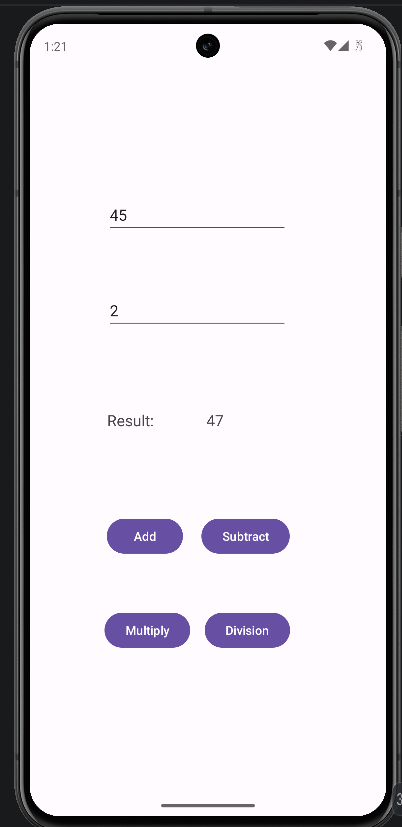
\includegraphics[width=0.4\textwidth]{Output_Screenshots/4_1.png} \quad 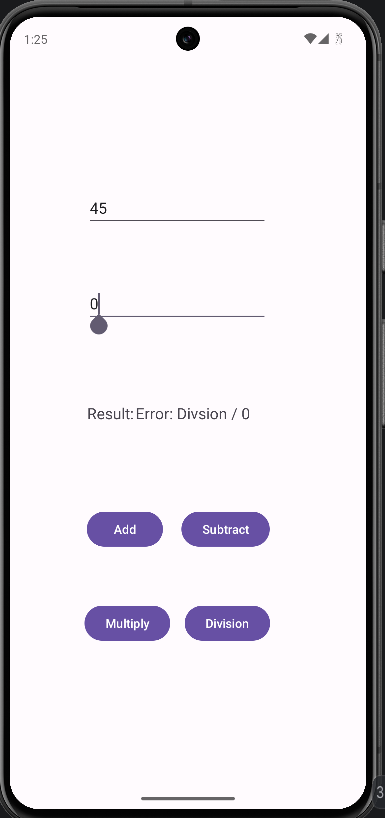
\includegraphics[width=0.4\textwidth]{Output_Screenshots/4_2.png} \end{center} \\
\end{longtable}
\endgroup

\newpage

%% ─── Program 5 ──────────────────────────────────────────────
\noindent\begingroup
\renewcommand{\arraystretch}{1.1}
\begin{longtable}{|p{0.94\textwidth}|}
\hline\endfirsthead\hline\endhead\hline\endfoot\hline\endlastfoot
\rule{0pt}{13pt}Program No: 5 \hfill Date: 29/06/2026 \\
\hline
\rule{0pt}{13pt}Program Title: Create an app that changes text color when a button is clicked. \\
\hline
\rule{0pt}{13pt}\textbf{MainActivity.java:} \\
\hline
{\ttfamily\small package\ com.example.pg05\_textcolor;} \\
\strut \\
{\ttfamily\small import\ android.graphics.Color;} \\
{\ttfamily\small import\ android.os.Bundle;} \\
\strut \\
{\ttfamily\small import\ androidx.activity.EdgeToEdge;} \\
{\ttfamily\small import\ androidx.appcompat.app.AppCompatActivity;} \\
{\ttfamily\small import\ androidx.core.graphics.Insets;} \\
{\ttfamily\small import\ androidx.core.view.ViewCompat;} \\
{\ttfamily\small import\ androidx.core.view.WindowInsetsCompat;} \\
{\ttfamily\small import\ android.widget.TextView;} \\
{\ttfamily\small import\ android.widget.Button;} \\
\strut \\
{\ttfamily\small public\ class\ MainActivity\ extends\ AppCompatActivity\ \{} \\
{\ttfamily\small \ \ \ \ TextView\ name;} \\
{\ttfamily\small \ \ \ \ Button\ color;} \\
{\ttfamily\small \ \ \ \ @Override} \\
{\ttfamily\small \ \ \ \ protected\ void\ onCreate(Bundle\ savedInstanceState)\ \{} \\
{\ttfamily\small \ \ \ \ \ \ \ \ super.onCreate(savedInstanceState);} \\
{\ttfamily\small \ \ \ \ \ \ \ \ EdgeToEdge.enable(this);} \\
{\ttfamily\small \ \ \ \ \ \ \ \ setContentView(R.layout.activity\_main);} \\
{\ttfamily\small \ \ \ \ \ \ \ \ color\ =\ findViewById(R.id.color);} \\
{\ttfamily\small \ \ \ \ \ \ \ \ name\ =\ findViewById(R.id.name);} \\
{\ttfamily\small \ \ \ \ \ \ \ \ color.setOnClickListener(v\ -\textgreater{}\ \{} \\
{\ttfamily\small \ \ \ \ \ \ \ \ \ \ \ \ name.setTextColor(Color.RED);} \\
{\ttfamily\small \ \ \ \ \ \ \ \ \});} \\
\strut \\
{\ttfamily\small \ \ \ \ \}} \\
{\ttfamily\small \}} \\
\hline
\rule{0pt}{13pt}\textbf{activity\_main.xml:} \\
\hline
{\ttfamily\small \textless{}?xml\ version="1.0"\ encoding="utf-8"?\textgreater{}} \\
{\ttfamily\small \textless{}androidx.constraintlayout.widget.ConstraintLayout\ xmlns:android="http://schemas.android.com/apk/res/android"} \\
{\ttfamily\small \ \ \ \ xmlns:app="http://schemas.android.com/apk/res-auto"} \\
{\ttfamily\small \ \ \ \ xmlns:tools="http://schemas.android.com/tools"} \\
{\ttfamily\small \ \ \ \ android:id="@+id/main"} \\
{\ttfamily\small \ \ \ \ android:layout\_width="match\_parent"} \\
{\ttfamily\small \ \ \ \ android:layout\_height="match\_parent"} \\
{\ttfamily\small \ \ \ \ tools:context=".MainActivity"\textgreater{}} \\
\strut \\
{\ttfamily\small \ \ \ \ \textless{}TextView} \\
{\ttfamily\small \ \ \ \ \ \ \ \ android:id="@+id/name"} \\
{\ttfamily\small \ \ \ \ \ \ \ \ android:layout\_width="wrap\_content"} \\
{\ttfamily\small \ \ \ \ \ \ \ \ android:layout\_height="wrap\_content"} \\
{\ttfamily\small \ \ \ \ \ \ \ \ android:text="Shyam"} \\
{\ttfamily\small \ \ \ \ \ \ \ \ android:textSize="24sp"} \\
{\ttfamily\small \ \ \ \ \ \ \ \ app:layout\_constraintBottom\_toBottomOf="parent"} \\
{\ttfamily\small \ \ \ \ \ \ \ \ app:layout\_constraintEnd\_toEndOf="parent"} \\
{\ttfamily\small \ \ \ \ \ \ \ \ app:layout\_constraintHorizontal\_bias="0.498"} \\
{\ttfamily\small \ \ \ \ \ \ \ \ app:layout\_constraintStart\_toStartOf="parent"} \\
{\ttfamily\small \ \ \ \ \ \ \ \ app:layout\_constraintTop\_toTopOf="parent"} \\
{\ttfamily\small \ \ \ \ \ \ \ \ app:layout\_constraintVertical\_bias="0.421"\ /\textgreater{}} \\
\strut \\
{\ttfamily\small \ \ \ \ \textless{}Button} \\
{\ttfamily\small \ \ \ \ \ \ \ \ android:id="@+id/color"} \\
{\ttfamily\small \ \ \ \ \ \ \ \ android:layout\_width="wrap\_content"} \\
{\ttfamily\small \ \ \ \ \ \ \ \ android:layout\_height="wrap\_content"} \\
{\ttfamily\small \ \ \ \ \ \ \ \ android:text="Change\ Color"} \\
{\ttfamily\small \ \ \ \ \ \ \ \ app:layout\_constraintBottom\_toBottomOf="parent"} \\
{\ttfamily\small \ \ \ \ \ \ \ \ app:layout\_constraintEnd\_toEndOf="parent"} \\
{\ttfamily\small \ \ \ \ \ \ \ \ app:layout\_constraintStart\_toStartOf="parent"} \\
{\ttfamily\small \ \ \ \ \ \ \ \ app:layout\_constraintTop\_toTopOf="parent"} \\
{\ttfamily\small \ \ \ \ \ \ \ \ app:layout\_constraintVertical\_bias="0.613"\ /\textgreater{}} \\
\strut \\
{\ttfamily\small \textless{}/androidx.constraintlayout.widget.ConstraintLayout\textgreater{}} \\
\hline
Output: \newline \begin{center} 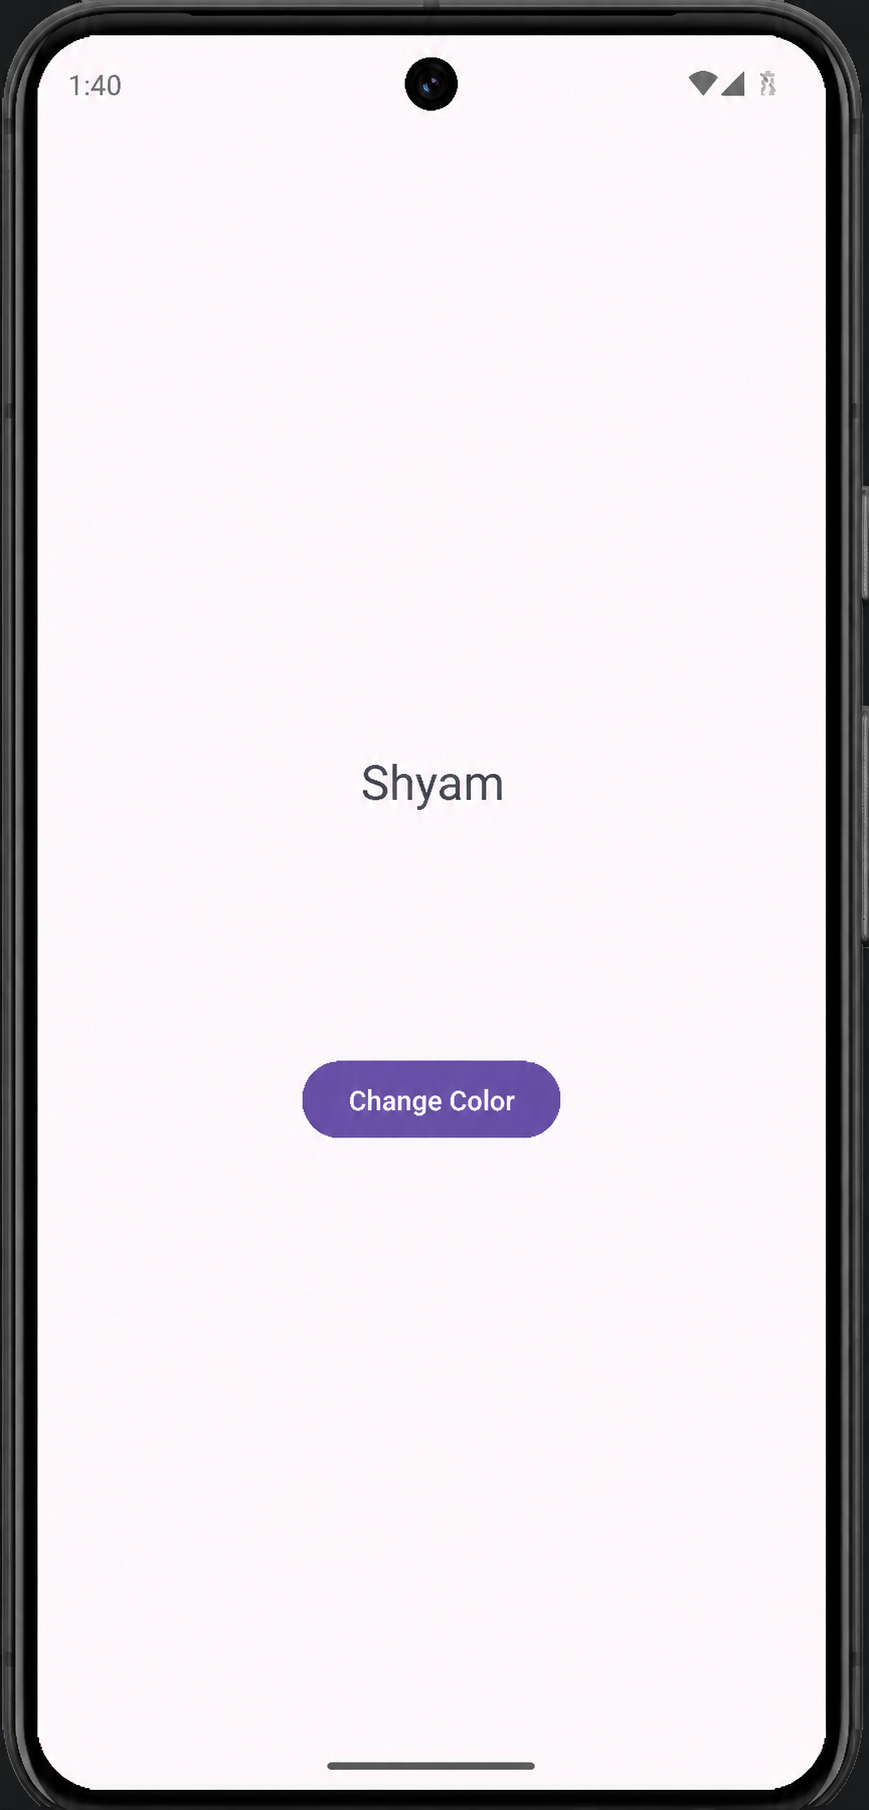
\includegraphics[width=0.4\textwidth]{Output_Screenshots/5_1.png} \quad 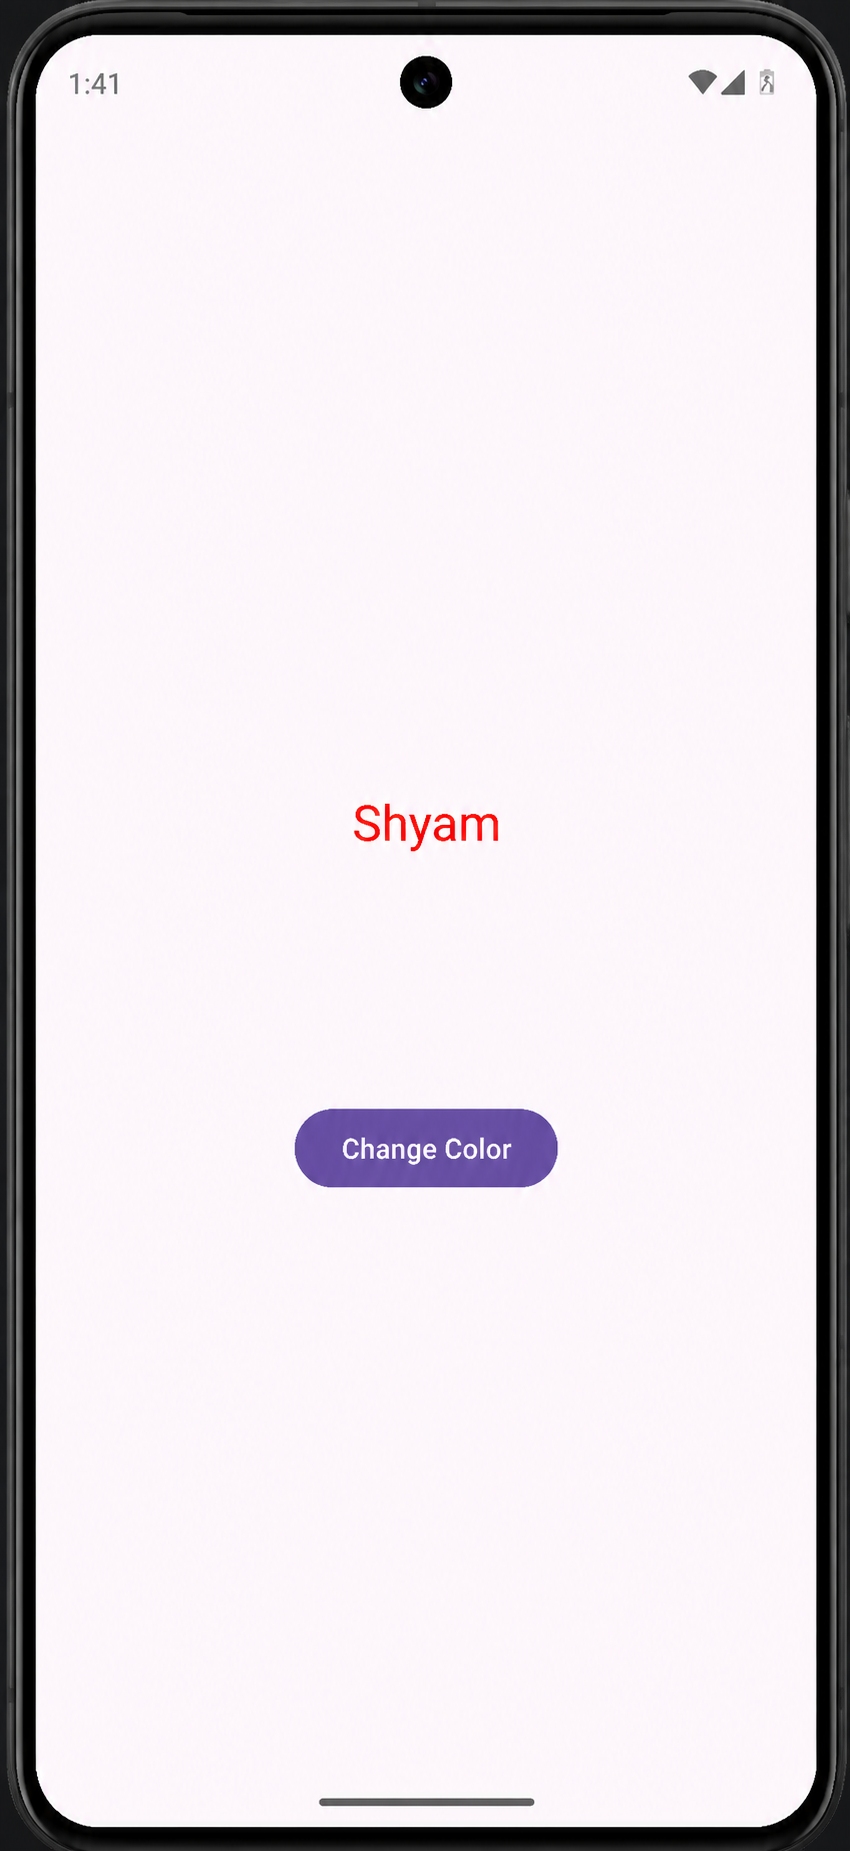
\includegraphics[width=0.4\textwidth]{Output_Screenshots/5_2.png} \end{center} \\
\end{longtable}
\endgroup

\newpage

%% ─── Program 6 ──────────────────────────────────────────────
\noindent\begingroup
\renewcommand{\arraystretch}{1.1}
\begin{longtable}{|p{0.94\textwidth}|}
\hline\endfirsthead\hline\endhead\hline\endfoot\hline\endlastfoot
\rule{0pt}{13pt}Program No: 6 \hfill Date: 29/06/2026 \\
\hline
\rule{0pt}{13pt}Program Title: Create an app that displays Date and Time in different formats using Linear Layout. \\
\hline
\rule{0pt}{13pt}\textbf{MainActivity.java:} \\
\hline
{\ttfamily\small package\ com.example.pg06\_datetime;} \\
\strut \\
{\ttfamily\small import\ android.os.Bundle;} \\
{\ttfamily\small import\ android.view.View;} \\
{\ttfamily\small import\ android.widget.Button;} \\
{\ttfamily\small import\ android.widget.TextView;} \\
{\ttfamily\small import\ androidx.appcompat.app.AppCompatActivity;} \\
{\ttfamily\small import\ java.text.SimpleDateFormat;} \\
{\ttfamily\small import\ java.util.Date;} \\
{\ttfamily\small import\ java.util.Locale;} \\
\strut \\
{\ttfamily\small public\ class\ MainActivity\ extends\ AppCompatActivity\ \{} \\
\strut \\
{\ttfamily\small \ \ \ \ @Override} \\
{\ttfamily\small \ \ \ \ protected\ void\ onCreate(Bundle\ savedInstanceState)\ \{} \\
{\ttfamily\small \ \ \ \ \ \ \ \ super.onCreate(savedInstanceState);} \\
{\ttfamily\small \ \ \ \ \ \ \ \ setContentView(R.layout.activity\_main);} \\
{\ttfamily\small \ \ \ \ \ \ \ \ final\ TextView\ textView1\ =\ findViewById(R.id.textView1);} \\
{\ttfamily\small \ \ \ \ \ \ \ \ final\ TextView\ textView2\ =\ findViewById(R.id.textView2);} \\
{\ttfamily\small \ \ \ \ \ \ \ \ final\ TextView\ textView3\ =\ findViewById(R.id.textView3);} \\
{\ttfamily\small \ \ \ \ \ \ \ \ final\ TextView\ textView4\ =\ findViewById(R.id.textView4);} \\
{\ttfamily\small \ \ \ \ \ \ \ \ Button\ button1\ =\ findViewById(R.id.button1);} \\
{\ttfamily\small \ \ \ \ \ \ \ \ button1.setOnClickListener(new\ View.OnClickListener()\ \{} \\
{\ttfamily\small \ \ \ \ \ \ \ \ \ \ \ \ @Override} \\
{\ttfamily\small \ \ \ \ \ \ \ \ \ \ \ \ public\ void\ onClick(View\ v)\ \{} \\
{\ttfamily\small \ \ \ \ \ \ \ \ \ \ \ \ \ \ \ \ Date\ currentDateTime\ =\ new\ Date();} \\
{\ttfamily\small \ \ \ \ \ \ \ \ \ \ \ \ \ \ \ \ SimpleDateFormat\ format1\ =\ new\ SimpleDateFormat("EEEE,\ dd\ MMM\ yyyy",\ Locale.getDefault());} \\
{\ttfamily\small \ \ \ \ \ \ \ \ \ \ \ \ \ \ \ \ SimpleDateFormat\ format2\ =\ new\ SimpleDateFormat("MM/dd/yyyy",\ Locale.getDefault());} \\
{\ttfamily\small \ \ \ \ \ \ \ \ \ \ \ \ \ \ \ \ SimpleDateFormat\ format3\ =\ new\ SimpleDateFormat("HH:mm:ss\ z",\ Locale.getDefault());} \\
{\ttfamily\small \ \ \ \ \ \ \ \ \ \ \ \ \ \ \ \ SimpleDateFormat\ format4\ =\ new\ SimpleDateFormat("hh:mm\ a",\ Locale.getDefault());} \\
{\ttfamily\small \ \ \ \ \ \ \ \ \ \ \ \ \ \ \ \ textView1.setText(format1.format(currentDateTime));} \\
{\ttfamily\small \ \ \ \ \ \ \ \ \ \ \ \ \ \ \ \ textView2.setText(format2.format(currentDateTime));} \\
{\ttfamily\small \ \ \ \ \ \ \ \ \ \ \ \ \ \ \ \ textView3.setText(format3.format(currentDateTime));} \\
{\ttfamily\small \ \ \ \ \ \ \ \ \ \ \ \ \ \ \ \ textView4.setText(format4.format(currentDateTime));} \\
{\ttfamily\small \ \ \ \ \ \ \ \ \ \ \ \ \}} \\
{\ttfamily\small \ \ \ \ \ \ \ \ \});} \\
{\ttfamily\small \ \ \ \ \}} \\
{\ttfamily\small \}} \\
\hline
\rule{0pt}{13pt}\textbf{activity\_main.xml:} \\
\hline
{\ttfamily\small \textless{}?xml\ version="1.0"\ encoding="utf-8"?\textgreater{}} \\
{\ttfamily\small \textless{}LinearLayout\ xmlns:android="http://schemas.android.com/apk/res/android"} \\
{\ttfamily\small \ \ \ \ xmlns:app="http://schemas.android.com/apk/res-auto"} \\
{\ttfamily\small \ \ \ \ xmlns:tools="http://schemas.android.com/tools"} \\
{\ttfamily\small \ \ \ \ android:id="@+id/main"} \\
{\ttfamily\small \ \ \ \ android:layout\_width="match\_parent"} \\
{\ttfamily\small \ \ \ \ android:layout\_height="match\_parent"} \\
{\ttfamily\small \ \ \ \ android:orientation="vertical"} \\
{\ttfamily\small \ \ \ \ android:gravity="center"} \\
{\ttfamily\small \ \ \ \ tools:context=".MainActivity"\textgreater{}} \\
\strut \\
{\ttfamily\small \ \ \ \ \textless{}TextView} \\
{\ttfamily\small \ \ \ \ \ \ \ \ android:id="@+id/textView1"} \\
{\ttfamily\small \ \ \ \ \ \ \ \ android:layout\_width="wrap\_content"} \\
{\ttfamily\small \ \ \ \ \ \ \ \ android:layout\_height="wrap\_content"} \\
{\ttfamily\small \ \ \ \ \ \ \ \ android:textSize="20sp"\ /\textgreater{}} \\
\strut \\
{\ttfamily\small \ \ \ \ \textless{}TextView} \\
{\ttfamily\small \ \ \ \ \ \ \ \ android:id="@+id/textView2"} \\
{\ttfamily\small \ \ \ \ \ \ \ \ android:layout\_width="wrap\_content"} \\
{\ttfamily\small \ \ \ \ \ \ \ \ android:layout\_height="wrap\_content"} \\
{\ttfamily\small \ \ \ \ \ \ \ \ android:textSize="20sp"\ /\textgreater{}} \\
\strut \\
{\ttfamily\small \ \ \ \ \textless{}TextView} \\
{\ttfamily\small \ \ \ \ \ \ \ \ android:id="@+id/textView3"} \\
{\ttfamily\small \ \ \ \ \ \ \ \ android:layout\_width="wrap\_content"} \\
{\ttfamily\small \ \ \ \ \ \ \ \ android:layout\_height="wrap\_content"} \\
{\ttfamily\small \ \ \ \ \ \ \ \ android:textSize="20sp"\ /\textgreater{}} \\
\strut \\
{\ttfamily\small \ \ \ \ \textless{}TextView} \\
{\ttfamily\small \ \ \ \ \ \ \ \ android:id="@+id/textView4"} \\
{\ttfamily\small \ \ \ \ \ \ \ \ android:layout\_width="wrap\_content"} \\
{\ttfamily\small \ \ \ \ \ \ \ \ android:layout\_height="wrap\_content"} \\
{\ttfamily\small \ \ \ \ \ \ \ \ android:textSize="20sp"\ /\textgreater{}} \\
{\ttfamily\small \ \ \ \ \textless{}Button} \\
{\ttfamily\small \ \ \ \ \ \ \ \ android:id="@+id/button1"} \\
{\ttfamily\small \ \ \ \ \ \ \ \ android:layout\_width="wrap\_content"} \\
{\ttfamily\small \ \ \ \ \ \ \ \ android:layout\_height="wrap\_content"} \\
{\ttfamily\small \ \ \ \ \ \ \ \ android:text="Button"\ /\textgreater{}} \\
\strut \\
{\ttfamily\small \textless{}/LinearLayout\textgreater{}} \\
\hline
Output: \newline \begin{center} 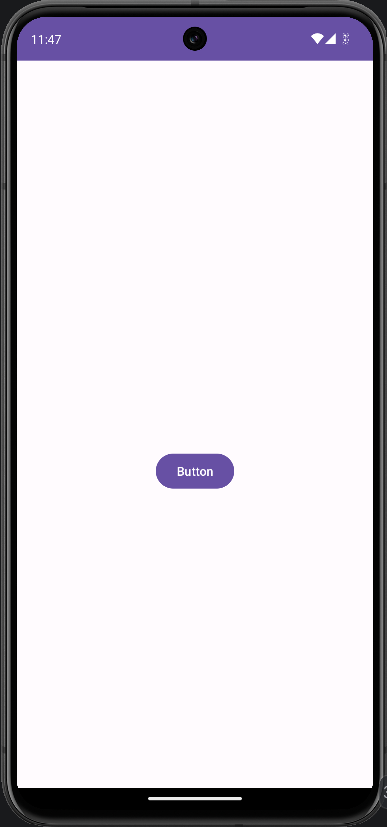
\includegraphics[width=0.4\textwidth]{Output_Screenshots/6_1.png} \quad 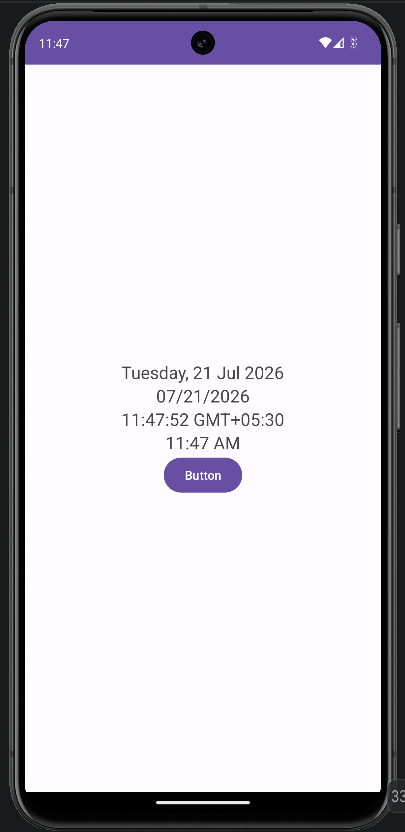
\includegraphics[width=0.4\textwidth]{Output_Screenshots/6_2.png} \end{center} \\
\end{longtable}
\endgroup

\newpage

%% ─── Program 7 ──────────────────────────────────────────────
\noindent\begingroup
\renewcommand{\arraystretch}{1.1}
\begin{longtable}{|p{0.94\textwidth}|}
\hline\endfirsthead\hline\endhead\hline\endfoot\hline\endlastfoot
\rule{0pt}{13pt}Program No: 7 \hfill Date: 29/06/2026 \\
\hline
\rule{0pt}{13pt}Program Title: Create an app that displays a Toast on the launch of an activity. \\
\hline
\rule{0pt}{13pt}\textbf{MainActivity.java:} \\
\hline
{\ttfamily\small package\ com.example.pg07\_launchtoast;} \\
\strut \\
{\ttfamily\small import\ android.os.Bundle;} \\
{\ttfamily\small import\ android.widget.Toast;} \\
{\ttfamily\small import\ androidx.activity.EdgeToEdge;} \\
{\ttfamily\small import\ androidx.appcompat.app.AppCompatActivity;} \\
{\ttfamily\small import\ androidx.core.graphics.Insets;} \\
{\ttfamily\small import\ androidx.core.view.ViewCompat;} \\
{\ttfamily\small import\ androidx.core.view.WindowInsetsCompat;} \\
\strut \\
{\ttfamily\small public\ class\ MainActivity\ extends\ AppCompatActivity\ \{} \\
{\ttfamily\small \ \ \ \ @Override} \\
{\ttfamily\small \ \ \ \ protected\ void\ onCreate(Bundle\ savedInstanceState)\ \{} \\
{\ttfamily\small \ \ \ \ \ \ \ \ super.onCreate(savedInstanceState);} \\
{\ttfamily\small \ \ \ \ \ \ \ \ EdgeToEdge.enable(this);} \\
{\ttfamily\small \ \ \ \ \ \ \ \ setContentView(R.layout.activity\_main);} \\
{\ttfamily\small \ \ \ \ \ \ \ \ Toast.makeText(this,\ "Welcome\ Shyam",\ Toast.LENGTH\_SHORT).show();} \\
{\ttfamily\small \ \ \ \ \}} \\
{\ttfamily\small \}} \\
\hline
\rule{0pt}{13pt}\textbf{activity\_main.xml:} \\
\hline
{\ttfamily\small \textless{}?xml\ version="1.0"\ encoding="utf-8"?\textgreater{}} \\
{\ttfamily\small \textless{}androidx.constraintlayout.widget.ConstraintLayout\ xmlns:android="http://schemas.android.com/apk/res/android"} \\
{\ttfamily\small \ \ \ \ xmlns:app="http://schemas.android.com/apk/res-auto"} \\
{\ttfamily\small \ \ \ \ xmlns:tools="http://schemas.android.com/tools"} \\
{\ttfamily\small \ \ \ \ android:id="@+id/main"} \\
{\ttfamily\small \ \ \ \ android:layout\_width="match\_parent"} \\
{\ttfamily\small \ \ \ \ android:layout\_height="match\_parent"} \\
{\ttfamily\small \ \ \ \ tools:context=".MainActivity"\textgreater{}} \\
\strut \\
{\ttfamily\small \ \ \ \ \textless{}TextView} \\
{\ttfamily\small \ \ \ \ \ \ \ \ android:layout\_width="wrap\_content"} \\
{\ttfamily\small \ \ \ \ \ \ \ \ android:layout\_height="wrap\_content"} \\
{\ttfamily\small \ \ \ \ \ \ \ \ android:text="Hello\ \ \^{}\_\^{}"} \\
{\ttfamily\small \ \ \ \ \ \ \ \ android:textSize="24sp"} \\
{\ttfamily\small \ \ \ \ \ \ \ \ app:layout\_constraintBottom\_toBottomOf="parent"} \\
{\ttfamily\small \ \ \ \ \ \ \ \ app:layout\_constraintEnd\_toEndOf="parent"} \\
{\ttfamily\small \ \ \ \ \ \ \ \ app:layout\_constraintStart\_toStartOf="parent"} \\
{\ttfamily\small \ \ \ \ \ \ \ \ app:layout\_constraintTop\_toTopOf="parent"\ /\textgreater{}} \\
\strut \\
{\ttfamily\small \textless{}/androidx.constraintlayout.widget.ConstraintLayout\textgreater{}} \\
\hline
Output: \newline \begin{center} 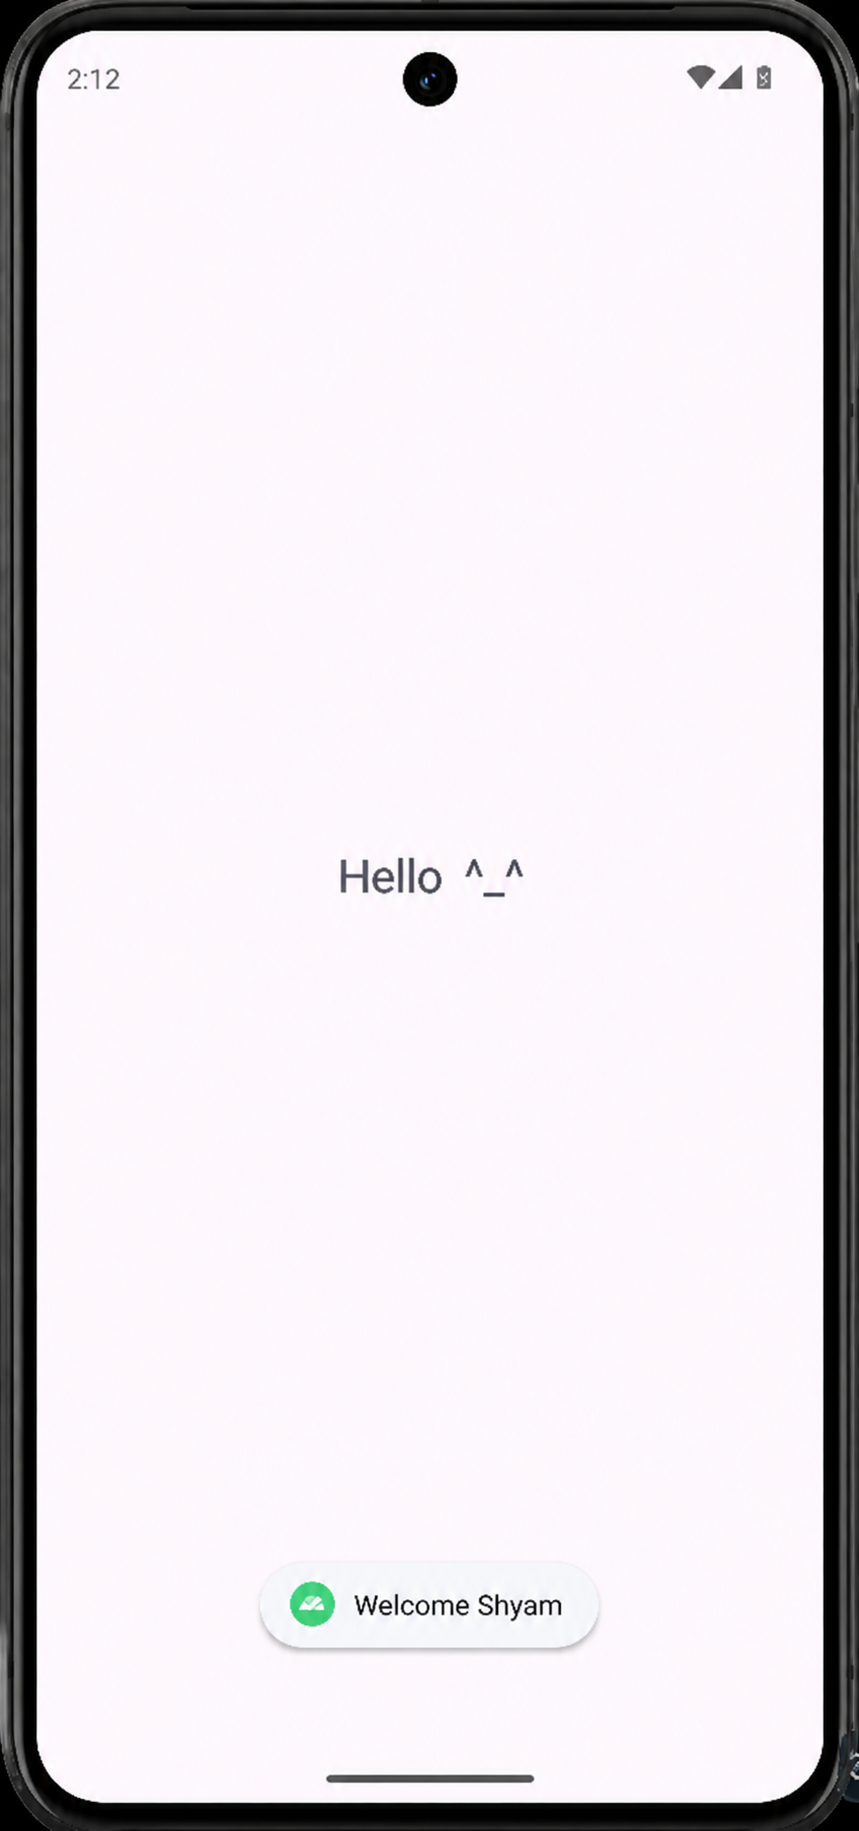
\includegraphics[width=0.45\textwidth]{Output_Screenshots/7.png} \end{center} \\
\end{longtable}
\endgroup

\newpage

%% ─── Program 8 ──────────────────────────────────────────────
\noindent\begingroup
\renewcommand{\arraystretch}{1.1}
\begin{longtable}{|p{0.94\textwidth}|}
\hline\endfirsthead\hline\endhead\hline\endfoot\hline\endlastfoot
\rule{0pt}{13pt}Program No: 8 \hfill Date: 29/06/2026 \\
\hline
\rule{0pt}{13pt}Program Title: Create an app that creates an Alert Dialog Box. \\
\hline
\rule{0pt}{13pt}\textbf{MainActivity.java:} \\
\hline
{\ttfamily\small package\ com.example.pg08\_alertbox;} \\
\strut \\
{\ttfamily\small import\ android.os.Bundle;} \\
{\ttfamily\small import\ androidx.appcompat.app.AppCompatActivity;} \\
{\ttfamily\small import\ androidx.appcompat.app.AlertDialog;} \\
{\ttfamily\small import\ android.widget.Button;} \\
{\ttfamily\small import\ android.widget.Toast;} \\
\strut \\
{\ttfamily\small public\ class\ MainActivity\ extends\ AppCompatActivity\ \{} \\
{\ttfamily\small \ \ \ \ @Override} \\
{\ttfamily\small \ \ \ \ protected\ void\ onCreate(Bundle\ savedInstanceState)\ \{} \\
{\ttfamily\small \ \ \ \ \ \ \ \ super.onCreate(savedInstanceState);} \\
{\ttfamily\small \ \ \ \ \ \ \ \ setContentView(R.layout.activity\_main);} \\
\strut \\
{\ttfamily\small \ \ \ \ \ \ \ \ Button\ btn\ =\ findViewById(R.id.btn);} \\
{\ttfamily\small \ \ \ \ \ \ \ \ btn.setOnClickListener(v\ -\textgreater{}\ \{} \\
{\ttfamily\small \ \ \ \ \ \ \ \ \ \ \ \ AlertDialog.Builder\ builder\ =\ new\ AlertDialog.Builder(MainActivity.this);} \\
{\ttfamily\small \ \ \ \ \ \ \ \ \ \ \ \ builder.setTitle("Alert");} \\
{\ttfamily\small \ \ \ \ \ \ \ \ \ \ \ \ builder.setMessage("What\ do\ you\ want\ to\ click?");} \\
\strut \\
{\ttfamily\small \ \ \ \ \ \ \ \ \ \ \ \ builder.setPositiveButton("Yes",\ (dialog,\ which)\ -\textgreater{}\ \{} \\
{\ttfamily\small \ \ \ \ \ \ \ \ \ \ \ \ \ \ \ \ Toast.makeText(MainActivity.this,\ "You\ clicked\ Yes",\ } \\
{\ttfamily\small \ \ \ \ \ \ \ \ \ \ \ \ \ \ \ \ \ \ \ \ \ \ \ \ \ \ \ \ \ \ \ Toast.LENGTH\_SHORT).show();} \\
{\ttfamily\small \ \ \ \ \ \ \ \ \ \ \ \ \});} \\
\strut \\
{\ttfamily\small \ \ \ \ \ \ \ \ \ \ \ \ builder.setNegativeButton("No",\ (dialog,\ which)\ -\textgreater{}\ \{} \\
{\ttfamily\small \ \ \ \ \ \ \ \ \ \ \ \ \ \ \ \ Toast.makeText(MainActivity.this,\ "You\ clicked\ No",\ } \\
{\ttfamily\small \ \ \ \ \ \ \ \ \ \ \ \ \ \ \ \ \ \ \ \ \ \ \ \ \ \ \ \ \ \ \ Toast.LENGTH\_SHORT).show();} \\
{\ttfamily\small \ \ \ \ \ \ \ \ \ \ \ \ \});} \\
\strut \\
{\ttfamily\small \ \ \ \ \ \ \ \ \ \ \ \ builder.setNeutralButton("Cancel",\ (dialog,\ which)\ -\textgreater{}\ \{} \\
{\ttfamily\small \ \ \ \ \ \ \ \ \ \ \ \ \ \ \ \ dialog.dismiss();} \\
{\ttfamily\small \ \ \ \ \ \ \ \ \ \ \ \ \});} \\
\strut \\
{\ttfamily\small \ \ \ \ \ \ \ \ \ \ \ \ builder.show();} \\
{\ttfamily\small \ \ \ \ \ \ \ \ \});} \\
{\ttfamily\small \ \ \ \ \}} \\
{\ttfamily\small \}} \\
\hline
\rule{0pt}{13pt}\textbf{activity\_main.xml:} \\
\hline
{\ttfamily\small \textless{}?xml\ version="1.0"\ encoding="utf-8"?\textgreater{}} \\
{\ttfamily\small \textless{}androidx.constraintlayout.widget.ConstraintLayout\ xmlns:android="http://schemas.android.com/apk/res/android"} \\
{\ttfamily\small \ \ \ \ xmlns:app="http://schemas.android.com/apk/res-auto"} \\
{\ttfamily\small \ \ \ \ xmlns:tools="http://schemas.android.com/tools"} \\
{\ttfamily\small \ \ \ \ android:id="@+id/main"} \\
{\ttfamily\small \ \ \ \ android:layout\_width="match\_parent"} \\
{\ttfamily\small \ \ \ \ android:layout\_height="match\_parent"} \\
{\ttfamily\small \ \ \ \ tools:context=".MainActivity"\textgreater{}} \\
\strut \\
{\ttfamily\small \ \ \ \ \textless{}Button} \\
{\ttfamily\small \ \ \ \ \ \ \ \ android:id="@+id/btn"} \\
{\ttfamily\small \ \ \ \ \ \ \ \ android:layout\_width="wrap\_content"} \\
{\ttfamily\small \ \ \ \ \ \ \ \ android:layout\_height="wrap\_content"} \\
{\ttfamily\small \ \ \ \ \ \ \ \ android:text="Click\ Here"} \\
{\ttfamily\small \ \ \ \ \ \ \ \ app:layout\_constraintBottom\_toBottomOf="parent"} \\
{\ttfamily\small \ \ \ \ \ \ \ \ app:layout\_constraintEnd\_toEndOf="parent"} \\
{\ttfamily\small \ \ \ \ \ \ \ \ app:layout\_constraintStart\_toStartOf="parent"} \\
{\ttfamily\small \ \ \ \ \ \ \ \ app:layout\_constraintTop\_toTopOf="parent"} \\
{\ttfamily\small \ \ \ \ \ \ \ \ app:layout\_constraintVertical\_bias="0.566"\ /\textgreater{}} \\
\strut \\
{\ttfamily\small \textless{}/androidx.constraintlayout.widget.ConstraintLayout\textgreater{}} \\
\hline
Output: \newline \begin{center} 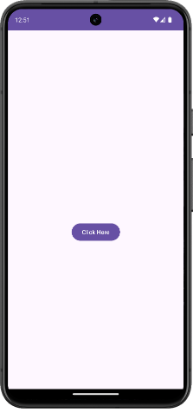
\includegraphics[width=0.3\textwidth]{Output_Screenshots/8_1.png} \quad 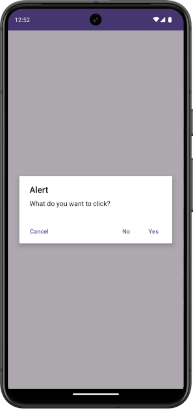
\includegraphics[width=0.3\textwidth]{Output_Screenshots/8_2.png} \quad 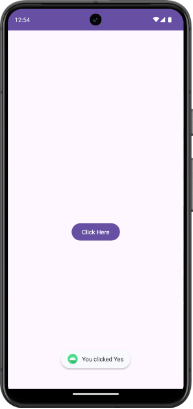
\includegraphics[width=0.3\textwidth]{Output_Screenshots/8_3.png} \end{center} \\
\end{longtable}
\endgroup

\newpage

%% ─── Program 9 ──────────────────────────────────────────────
\noindent\begingroup
\renewcommand{\arraystretch}{1.1}
\begin{longtable}{|p{0.94\textwidth}|}
\hline\endfirsthead\hline\endhead\hline\endfoot\hline\endlastfoot
\rule{0pt}{13pt}Program No: 9 \hfill Date: 29/06/2026 \\
\hline
\rule{0pt}{13pt}Program Title: Create a Greeting card app that displays an image. \\
\hline
\rule{0pt}{13pt}\textbf{MainActivity.java:} \\
\hline
{\ttfamily\small package\ com.example.pg09\_greetingcard;} \\
\strut \\
{\ttfamily\small import\ android.os.Bundle;} \\
{\ttfamily\small import\ androidx.appcompat.app.AppCompatActivity;} \\
\strut \\
{\ttfamily\small public\ class\ MainActivity\ extends\ AppCompatActivity\ \{} \\
{\ttfamily\small \ \ \ \ @Override} \\
{\ttfamily\small \ \ \ \ protected\ void\ onCreate(Bundle\ savedInstanceState)\ \{} \\
{\ttfamily\small \ \ \ \ \ \ \ \ super.onCreate(savedInstanceState);} \\
{\ttfamily\small \ \ \ \ \ \ \ \ setContentView(R.layout.activity\_main);} \\
{\ttfamily\small \ \ \ \ \}} \\
{\ttfamily\small \}} \\
\hline
\rule{0pt}{13pt}\textbf{activity\_main.xml:} \\
\hline
{\ttfamily\small \textless{}?xml\ version="1.0"\ encoding="utf-8"?\textgreater{}} \\
{\ttfamily\small \textless{}androidx.constraintlayout.widget.ConstraintLayout\ xmlns:android="http://schemas.android.com/apk/res/android"} \\
{\ttfamily\small \ \ \ \ xmlns:app="http://schemas.android.com/apk/res-auto"} \\
{\ttfamily\small \ \ \ \ xmlns:tools="http://schemas.android.com/tools"} \\
{\ttfamily\small \ \ \ \ android:id="@+id/main"} \\
{\ttfamily\small \ \ \ \ android:layout\_width="match\_parent"} \\
{\ttfamily\small \ \ \ \ android:layout\_height="match\_parent"} \\
{\ttfamily\small \ \ \ \ tools:context=".MainActivity"\textgreater{}} \\
\strut \\
{\ttfamily\small \ \ \ \ \textless{}ImageView} \\
{\ttfamily\small \ \ \ \ \ \ \ \ android:id="@+id/imageView"} \\
{\ttfamily\small \ \ \ \ \ \ \ \ android:layout\_width="288dp"} \\
{\ttfamily\small \ \ \ \ \ \ \ \ android:layout\_height="393dp"} \\
{\ttfamily\small \ \ \ \ \ \ \ \ app:layout\_constraintBottom\_toBottomOf="parent"} \\
{\ttfamily\small \ \ \ \ \ \ \ \ app:layout\_constraintEnd\_toEndOf="parent"} \\
{\ttfamily\small \ \ \ \ \ \ \ \ app:layout\_constraintHorizontal\_bias="0.495"} \\
{\ttfamily\small \ \ \ \ \ \ \ \ app:layout\_constraintStart\_toStartOf="parent"} \\
{\ttfamily\small \ \ \ \ \ \ \ \ app:layout\_constraintTop\_toTopOf="parent"} \\
{\ttfamily\small \ \ \ \ \ \ \ \ app:layout\_constraintVertical\_bias="0.328"} \\
{\ttfamily\small \ \ \ \ \ \ \ \ app:srcCompat="@drawable/greetings"\ /\textgreater{}} \\
\strut \\
{\ttfamily\small \ \ \ \ \textless{}TextView} \\
{\ttfamily\small \ \ \ \ \ \ \ \ android:id="@+id/textView2"} \\
{\ttfamily\small \ \ \ \ \ \ \ \ android:layout\_width="wrap\_content"} \\
{\ttfamily\small \ \ \ \ \ \ \ \ android:layout\_height="wrap\_content"} \\
{\ttfamily\small \ \ \ \ \ \ \ \ android:text="Happy\ Birthday!"} \\
{\ttfamily\small \ \ \ \ \ \ \ \ android:textColor="\#2196F3"} \\
{\ttfamily\small \ \ \ \ \ \ \ \ android:textSize="24sp"} \\
{\ttfamily\small \ \ \ \ \ \ \ \ app:layout\_constraintBottom\_toBottomOf="parent"} \\
{\ttfamily\small \ \ \ \ \ \ \ \ app:layout\_constraintEnd\_toEndOf="parent"} \\
{\ttfamily\small \ \ \ \ \ \ \ \ app:layout\_constraintStart\_toStartOf="parent"} \\
{\ttfamily\small \ \ \ \ \ \ \ \ app:layout\_constraintTop\_toTopOf="parent"} \\
{\ttfamily\small \ \ \ \ \ \ \ \ app:layout\_constraintVertical\_bias="0.739"\ /\textgreater{}} \\
\strut \\
{\ttfamily\small \ \ \ \ \textless{}TextView} \\
{\ttfamily\small \ \ \ \ \ \ \ \ android:id="@+id/textView"} \\
{\ttfamily\small \ \ \ \ \ \ \ \ android:layout\_width="258dp"} \\
{\ttfamily\small \ \ \ \ \ \ \ \ android:layout\_height="59dp"} \\
{\ttfamily\small \ \ \ \ \ \ \ \ android:text="Wishing\ you\ a\ joyful\ day\ and\ an\ amazing\ year\ ahead!"} \\
{\ttfamily\small \ \ \ \ \ \ \ \ android:textAlignment="center"} \\
{\ttfamily\small \ \ \ \ \ \ \ \ android:textColor="\#020202"} \\
{\ttfamily\small \ \ \ \ \ \ \ \ android:textSize="18sp"} \\
{\ttfamily\small \ \ \ \ \ \ \ \ app:layout\_constraintBottom\_toBottomOf="parent"} \\
{\ttfamily\small \ \ \ \ \ \ \ \ app:layout\_constraintEnd\_toEndOf="parent"} \\
{\ttfamily\small \ \ \ \ \ \ \ \ app:layout\_constraintHorizontal\_bias="0.496"} \\
{\ttfamily\small \ \ \ \ \ \ \ \ app:layout\_constraintStart\_toStartOf="parent"} \\
{\ttfamily\small \ \ \ \ \ \ \ \ app:layout\_constraintTop\_toTopOf="parent"} \\
{\ttfamily\small \ \ \ \ \ \ \ \ app:layout\_constraintVertical\_bias="0.833"\ /\textgreater{}} \\
\strut \\
{\ttfamily\small \textless{}/androidx.constraintlayout.widget.ConstraintLayout\textgreater{}} \\
\hline
Output: \newline \begin{center} 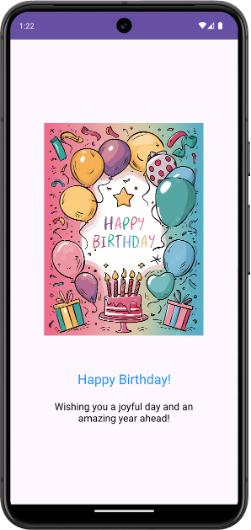
\includegraphics[width=0.45\textwidth]{Output_Screenshots/9.png} \end{center} \\
\end{longtable}
\endgroup

\newpage

%% ─── Program 10 ──────────────────────────────────────────────
\noindent\begingroup
\renewcommand{\arraystretch}{1.1}
\begin{longtable}{|p{0.94\textwidth}|}
\hline\endfirsthead\hline\endhead\hline\endfoot\hline\endlastfoot
\rule{0pt}{13pt}Program No: 10 \hfill Date: 29/06/2026 \\
\hline
\rule{0pt}{13pt}Program Title: Create an app that plays audio when we click on the button ``Play Music" and plays video when we click on the button ``Play Video". \\
\hline
\rule{0pt}{13pt}\textbf{MainActivity.java:} \\
\hline
{\ttfamily\small package\ com.example.pg10\_videomusic;} \\
\strut \\
{\ttfamily\small import\ android.os.Bundle;} \\
{\ttfamily\small import\ androidx.appcompat.app.AppCompatActivity;} \\
{\ttfamily\small import\ android.widget.Button;} \\
{\ttfamily\small import\ android.widget.VideoView;} \\
{\ttfamily\small import\ android.net.Uri;} \\
{\ttfamily\small import\ android.media.MediaPlayer;} \\
{\ttfamily\small import\ android.widget.MediaController;} \\
\strut \\
{\ttfamily\small public\ class\ MainActivity\ extends\ AppCompatActivity\ \{} \\
{\ttfamily\small \ \ \ \ MediaPlayer\ mediaPlayer;} \\
{\ttfamily\small \ \ \ \ VideoView\ videoView;} \\
\strut \\
{\ttfamily\small \ \ \ \ @Override} \\
{\ttfamily\small \ \ \ \ protected\ void\ onCreate(Bundle\ savedInstanceState)\ \{} \\
{\ttfamily\small \ \ \ \ \ \ \ \ super.onCreate(savedInstanceState);} \\
{\ttfamily\small \ \ \ \ \ \ \ \ setContentView(R.layout.activity\_main);} \\
\strut \\
{\ttfamily\small \ \ \ \ \ \ \ \ Button\ btnMusic\ =\ findViewById(R.id.music);} \\
{\ttfamily\small \ \ \ \ \ \ \ \ Button\ btnVideo\ =\ findViewById(R.id.video);} \\
\strut \\
{\ttfamily\small \ \ \ \ \ \ \ \ videoView\ =\ findViewById(R.id.videoView);} \\
{\ttfamily\small \ \ \ \ \ \ \ \ videoView.setZOrderOnTop(true);} \\
\strut \\
{\ttfamily\small \ \ \ \ \ \ \ \ mediaPlayer\ =\ MediaPlayer.create(this,\ R.raw.song);} \\
\strut \\
{\ttfamily\small \ \ \ \ \ \ \ \ btnMusic.setOnClickListener(v\ -\textgreater{}\ \{} \\
{\ttfamily\small \ \ \ \ \ \ \ \ \ \ \ \ if\ (!mediaPlayer.isPlaying())\ \{} \\
{\ttfamily\small \ \ \ \ \ \ \ \ \ \ \ \ \ \ \ \ mediaPlayer.start();} \\
{\ttfamily\small \ \ \ \ \ \ \ \ \ \ \ \ \}} \\
{\ttfamily\small \ \ \ \ \ \ \ \ \});} \\
\strut \\
{\ttfamily\small \ \ \ \ \ \ \ \ btnVideo.setOnClickListener(v\ -\textgreater{}\ \{} \\
{\ttfamily\small \ \ \ \ \ \ \ \ \ \ \ \ Uri\ uri\ =\ Uri.parse("android.resource://"\ +\ getPackageName()\ } \\
{\ttfamily\small \ \ \ \ \ \ \ \ \ \ \ \ \ \ \ \ \ \ \ \ \ \ \ \ \ \ \ \ \ \ \ \ +\ "/"\ +\ R.raw.video);} \\
{\ttfamily\small \ \ \ \ \ \ \ \ \ \ \ \ videoView.setVideoURI(uri);} \\
{\ttfamily\small \ \ \ \ \ \ \ \ \ \ \ \ MediaController\ controller\ =\ } \\
{\ttfamily\small \ \ \ \ \ \ \ \ \ \ \ \ \ \ \ \ \ \ \ \ new\ MediaController(MainActivity.this);} \\
{\ttfamily\small \ \ \ \ \ \ \ \ \ \ \ \ videoView.setMediaController(controller);} \\
{\ttfamily\small \ \ \ \ \ \ \ \ \ \ \ \ controller.setAnchorView(videoView);} \\
{\ttfamily\small \ \ \ \ \ \ \ \ \ \ \ \ videoView.start();} \\
{\ttfamily\small \ \ \ \ \ \ \ \ \});} \\
{\ttfamily\small \ \ \ \ \}} \\
\strut \\
{\ttfamily\small \ \ \ \ @Override} \\
{\ttfamily\small \ \ \ \ protected\ void\ onDestroy()\ \{} \\
{\ttfamily\small \ \ \ \ \ \ \ \ super.onDestroy();} \\
{\ttfamily\small \ \ \ \ \ \ \ \ if\ (mediaPlayer\ !=\ null)\ \{} \\
{\ttfamily\small \ \ \ \ \ \ \ \ \ \ \ \ mediaPlayer.release();} \\
{\ttfamily\small \ \ \ \ \ \ \ \ \ \ \ \ mediaPlayer\ =\ null;} \\
{\ttfamily\small \ \ \ \ \ \ \ \ \}} \\
{\ttfamily\small \ \ \ \ \}} \\
{\ttfamily\small \}} \\
\hline
\rule{0pt}{13pt}\textbf{activity\_main.xml:} \\
\hline
{\ttfamily\small \textless{}?xml\ version="1.0"\ encoding="utf-8"?\textgreater{}} \\
{\ttfamily\small \textless{}androidx.constraintlayout.widget.ConstraintLayout\ xmlns:android="http://schemas.android.com/apk/res/android"} \\
{\ttfamily\small \ \ \ \ xmlns:app="http://schemas.android.com/apk/res-auto"} \\
{\ttfamily\small \ \ \ \ xmlns:tools="http://schemas.android.com/tools"} \\
{\ttfamily\small \ \ \ \ android:id="@+id/main"} \\
{\ttfamily\small \ \ \ \ android:layout\_width="match\_parent"} \\
{\ttfamily\small \ \ \ \ android:layout\_height="match\_parent"} \\
{\ttfamily\small \ \ \ \ tools:context=".MainActivity"\textgreater{}} \\
\strut \\
{\ttfamily\small \ \ \ \ \textless{}VideoView} \\
{\ttfamily\small \ \ \ \ \ \ \ \ android:id="@+id/videoView"} \\
{\ttfamily\small \ \ \ \ \ \ \ \ android:layout\_width="348dp"} \\
{\ttfamily\small \ \ \ \ \ \ \ \ android:layout\_height="231dp"} \\
{\ttfamily\small \ \ \ \ \ \ \ \ android:background="\#000000"} \\
{\ttfamily\small \ \ \ \ \ \ \ \ app:layout\_constraintBottom\_toBottomOf="parent"} \\
{\ttfamily\small \ \ \ \ \ \ \ \ app:layout\_constraintEnd\_toEndOf="parent"} \\
{\ttfamily\small \ \ \ \ \ \ \ \ app:layout\_constraintHorizontal\_bias="0.492"} \\
{\ttfamily\small \ \ \ \ \ \ \ \ app:layout\_constraintStart\_toStartOf="parent"} \\
{\ttfamily\small \ \ \ \ \ \ \ \ app:layout\_constraintTop\_toTopOf="parent"} \\
{\ttfamily\small \ \ \ \ \ \ \ \ app:layout\_constraintVertical\_bias="0.23"\ /\textgreater{}} \\
\strut \\
{\ttfamily\small \ \ \ \ \textless{}Button} \\
{\ttfamily\small \ \ \ \ \ \ \ \ android:id="@+id/music"} \\
{\ttfamily\small \ \ \ \ \ \ \ \ android:layout\_width="wrap\_content"} \\
{\ttfamily\small \ \ \ \ \ \ \ \ android:layout\_height="wrap\_content"} \\
{\ttfamily\small \ \ \ \ \ \ \ \ android:text="Play\ Music"} \\
{\ttfamily\small \ \ \ \ \ \ \ \ app:layout\_constraintBottom\_toBottomOf="parent"} \\
{\ttfamily\small \ \ \ \ \ \ \ \ app:layout\_constraintEnd\_toEndOf="parent"} \\
{\ttfamily\small \ \ \ \ \ \ \ \ app:layout\_constraintHorizontal\_bias="0.237"} \\
{\ttfamily\small \ \ \ \ \ \ \ \ app:layout\_constraintStart\_toStartOf="parent"} \\
{\ttfamily\small \ \ \ \ \ \ \ \ app:layout\_constraintTop\_toTopOf="parent"} \\
{\ttfamily\small \ \ \ \ \ \ \ \ app:layout\_constraintVertical\_bias="0.632"\ /\textgreater{}} \\
\strut \\
{\ttfamily\small \ \ \ \ \textless{}Button} \\
{\ttfamily\small \ \ \ \ \ \ \ \ android:id="@+id/video"} \\
{\ttfamily\small \ \ \ \ \ \ \ \ android:layout\_width="wrap\_content"} \\
{\ttfamily\small \ \ \ \ \ \ \ \ android:layout\_height="wrap\_content"} \\
{\ttfamily\small \ \ \ \ \ \ \ \ android:layout\_marginStart="8dp"} \\
{\ttfamily\small \ \ \ \ \ \ \ \ android:text="Play\ Video"} \\
{\ttfamily\small \ \ \ \ \ \ \ \ app:layout\_constraintBottom\_toBottomOf="parent"} \\
{\ttfamily\small \ \ \ \ \ \ \ \ app:layout\_constraintEnd\_toEndOf="parent"} \\
{\ttfamily\small \ \ \ \ \ \ \ \ app:layout\_constraintHorizontal\_bias="0.777"} \\
{\ttfamily\small \ \ \ \ \ \ \ \ app:layout\_constraintStart\_toStartOf="parent"} \\
{\ttfamily\small \ \ \ \ \ \ \ \ app:layout\_constraintTop\_toTopOf="parent"} \\
{\ttfamily\small \ \ \ \ \ \ \ \ app:layout\_constraintVertical\_bias="0.632"\ /\textgreater{}} \\
\strut \\
{\ttfamily\small \textless{}/androidx.constraintlayout.widget.ConstraintLayout\textgreater{}} \\
\hline
Output: \newline \begin{center} 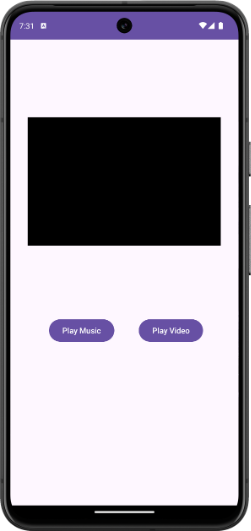
\includegraphics[width=0.4\textwidth]{Output_Screenshots/10_1.png} \quad 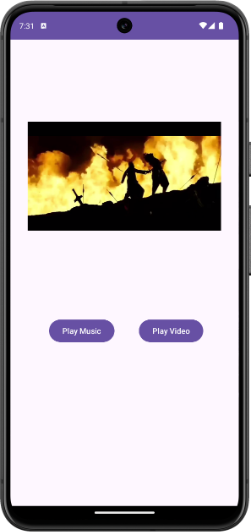
\includegraphics[width=0.4\textwidth]{Output_Screenshots/10_2.png} \end{center} \\
\end{longtable}
\endgroup

\newpage

%% ─── Program 11 ──────────────────────────────────────────────
\noindent\begingroup
\renewcommand{\arraystretch}{1.1}
\begin{longtable}{|p{0.94\textwidth}|}
\hline\endfirsthead\hline\endhead\hline\endfoot\hline\endlastfoot
\rule{0pt}{13pt}Program No: 11 \hfill Date: 29/06/2026 \\
\hline
\rule{0pt}{13pt}Program Title: Create an app that plays video from the internet. \\
\hline
\rule{0pt}{13pt}\textbf{MainActivity.java:} \\
\hline
{\ttfamily\small package\ com.example.pg11\_internetvideo;} \\
\strut \\
{\ttfamily\small import\ android.os.Bundle;} \\
{\ttfamily\small import\ androidx.appcompat.app.AppCompatActivity;} \\
{\ttfamily\small import\ android.widget.Button;} \\
{\ttfamily\small import\ android.widget.VideoView;} \\
{\ttfamily\small import\ android.net.Uri;} \\
{\ttfamily\small import\ android.widget.MediaController;} \\
\strut \\
{\ttfamily\small public\ class\ MainActivity\ extends\ AppCompatActivity\ \{} \\
{\ttfamily\small \ \ \ \ VideoView\ videoView;} \\
\strut \\
{\ttfamily\small \ \ \ \ @Override} \\
{\ttfamily\small \ \ \ \ protected\ void\ onCreate(Bundle\ savedInstanceState)\ \{} \\
{\ttfamily\small \ \ \ \ \ \ \ \ super.onCreate(savedInstanceState);} \\
{\ttfamily\small \ \ \ \ \ \ \ \ setContentView(R.layout.activity\_main);} \\
\strut \\
{\ttfamily\small \ \ \ \ \ \ \ \ Button\ btnVideo\ =\ findViewById(R.id.play);} \\
{\ttfamily\small \ \ \ \ \ \ \ \ videoView\ =\ findViewById(R.id.videoView);} \\
{\ttfamily\small \ \ \ \ \ \ \ \ videoView.setZOrderOnTop(true);} \\
\strut \\
{\ttfamily\small \ \ \ \ \ \ \ \ btnVideo.setOnClickListener(v\ -\textgreater{}\ \{} \\
{\ttfamily\small \ \ \ \ \ \ \ \ \ \ \ \ Uri\ uri\ =\ Uri.parse("https://www.learningcontainer.com/"} \\
{\ttfamily\small \ \ \ \ \ \ \ \ \ \ \ \ \ \ \ \ \ \ \ \ \ \ \ \ \ \ \ \ \ \ \ \ +\ "wp-content/uploads/2020/05/"} \\
{\ttfamily\small \ \ \ \ \ \ \ \ \ \ \ \ \ \ \ \ \ \ \ \ \ \ \ \ \ \ \ \ \ \ \ \ +\ "sample-mp4-file.mp4");} \\
{\ttfamily\small \ \ \ \ \ \ \ \ \ \ \ \ videoView.setVideoURI(uri);} \\
{\ttfamily\small \ \ \ \ \ \ \ \ \ \ \ \ MediaController\ controller\ =\ } \\
{\ttfamily\small \ \ \ \ \ \ \ \ \ \ \ \ \ \ \ \ \ \ \ \ new\ MediaController(MainActivity.this);} \\
{\ttfamily\small \ \ \ \ \ \ \ \ \ \ \ \ videoView.setMediaController(controller);} \\
{\ttfamily\small \ \ \ \ \ \ \ \ \ \ \ \ controller.setAnchorView(videoView);} \\
{\ttfamily\small \ \ \ \ \ \ \ \ \ \ \ \ videoView.start();} \\
{\ttfamily\small \ \ \ \ \ \ \ \ \});} \\
{\ttfamily\small \ \ \ \ \}} \\
{\ttfamily\small \}} \\
\hline
\rule{0pt}{13pt}\textbf{activity\_main.xml:} \\
\hline
{\ttfamily\small \textless{}?xml\ version="1.0"\ encoding="utf-8"?\textgreater{}} \\
{\ttfamily\small \textless{}androidx.constraintlayout.widget.ConstraintLayout\ xmlns:android="http://schemas.android.com/apk/res/android"} \\
{\ttfamily\small \ \ \ \ xmlns:app="http://schemas.android.com/apk/res-auto"} \\
{\ttfamily\small \ \ \ \ xmlns:tools="http://schemas.android.com/tools"} \\
{\ttfamily\small \ \ \ \ android:id="@+id/main"} \\
{\ttfamily\small \ \ \ \ android:layout\_width="match\_parent"} \\
{\ttfamily\small \ \ \ \ android:layout\_height="match\_parent"} \\
{\ttfamily\small \ \ \ \ tools:context=".MainActivity"\textgreater{}} \\
\strut \\
{\ttfamily\small \ \ \ \ \textless{}VideoView} \\
{\ttfamily\small \ \ \ \ \ \ \ \ android:id="@+id/videoView"} \\
{\ttfamily\small \ \ \ \ \ \ \ \ android:layout\_width="365dp"} \\
{\ttfamily\small \ \ \ \ \ \ \ \ android:layout\_height="211dp"} \\
{\ttfamily\small \ \ \ \ \ \ \ \ app:layout\_constraintBottom\_toBottomOf="parent"} \\
{\ttfamily\small \ \ \ \ \ \ \ \ app:layout\_constraintEnd\_toEndOf="parent"} \\
{\ttfamily\small \ \ \ \ \ \ \ \ app:layout\_constraintHorizontal\_bias="0.493"} \\
{\ttfamily\small \ \ \ \ \ \ \ \ app:layout\_constraintStart\_toStartOf="parent"} \\
{\ttfamily\small \ \ \ \ \ \ \ \ app:layout\_constraintTop\_toTopOf="parent"} \\
{\ttfamily\small \ \ \ \ \ \ \ \ app:layout\_constraintVertical\_bias="0.141"\ /\textgreater{}} \\
\strut \\
{\ttfamily\small \ \ \ \ \textless{}Button} \\
{\ttfamily\small \ \ \ \ \ \ \ \ android:id="@+id/play"} \\
{\ttfamily\small \ \ \ \ \ \ \ \ android:layout\_width="wrap\_content"} \\
{\ttfamily\small \ \ \ \ \ \ \ \ android:layout\_height="wrap\_content"} \\
{\ttfamily\small \ \ \ \ \ \ \ \ android:text="Play\ Video"} \\
{\ttfamily\small \ \ \ \ \ \ \ \ app:layout\_constraintBottom\_toBottomOf="parent"} \\
{\ttfamily\small \ \ \ \ \ \ \ \ app:layout\_constraintEnd\_toEndOf="parent"} \\
{\ttfamily\small \ \ \ \ \ \ \ \ app:layout\_constraintStart\_toStartOf="parent"} \\
{\ttfamily\small \ \ \ \ \ \ \ \ app:layout\_constraintTop\_toTopOf="parent"} \\
{\ttfamily\small \ \ \ \ \ \ \ \ app:layout\_constraintVertical\_bias="0.537"\ /\textgreater{}} \\
\strut \\
{\ttfamily\small \textless{}/androidx.constraintlayout.widget.ConstraintLayout\textgreater{}} \\
\hline
Output: \newline \begin{center} 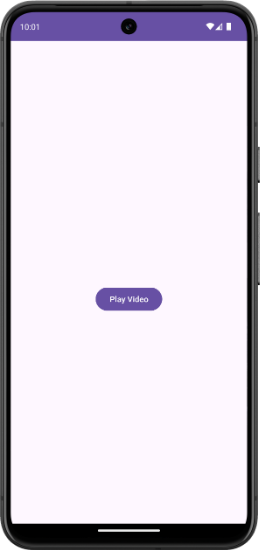
\includegraphics[width=0.4\textwidth]{Output_Screenshots/11_1.png} \quad 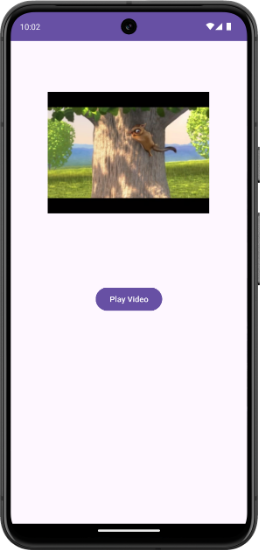
\includegraphics[width=0.4\textwidth]{Output_Screenshots/11_2.png} \end{center} \\
\end{longtable}
\endgroup

\newpage

%% ─── Program 12 ──────────────────────────────────────────────
\noindent\begingroup
\renewcommand{\arraystretch}{1.1}
\begin{longtable}{|p{0.94\textwidth}|}
\hline\endfirsthead\hline\endhead\hline\endfoot\hline\endlastfoot
\rule{0pt}{13pt}Program No: 12 \hfill Date: 29/06/2026 \\
\hline
\rule{0pt}{13pt}Program Title: Create an app to demonstrate Options Menu. \\
\hline
\rule{0pt}{13pt}\textbf{MainActivity.java:} \\
\hline
{\ttfamily\small package\ com.example.pg12\_optionsmenu;} \\
\strut \\
{\ttfamily\small import\ android.os.Bundle;} \\
{\ttfamily\small import\ androidx.appcompat.app.AppCompatActivity;} \\
{\ttfamily\small import\ android.view.Menu;} \\
{\ttfamily\small import\ android.view.MenuItem;} \\
{\ttfamily\small import\ android.widget.Toast;} \\
\strut \\
{\ttfamily\small public\ class\ MainActivity\ extends\ AppCompatActivity\ \{} \\
{\ttfamily\small \ \ \ \ @Override} \\
{\ttfamily\small \ \ \ \ protected\ void\ onCreate(Bundle\ savedInstanceState)\ \{} \\
{\ttfamily\small \ \ \ \ \ \ \ \ super.onCreate(savedInstanceState);} \\
{\ttfamily\small \ \ \ \ \ \ \ \ setContentView(R.layout.activity\_main);} \\
{\ttfamily\small \ \ \ \ \}} \\
\strut \\
{\ttfamily\small \ \ \ \ @Override} \\
{\ttfamily\small \ \ \ \ public\ boolean\ onCreateOptionsMenu(Menu\ menu)\ \{} \\
{\ttfamily\small \ \ \ \ \ \ \ \ getMenuInflater().inflate(R.menu.menu,\ menu);} \\
{\ttfamily\small \ \ \ \ \ \ \ \ return\ true;} \\
{\ttfamily\small \ \ \ \ \}} \\
\strut \\
{\ttfamily\small \ \ \ \ @Override} \\
{\ttfamily\small \ \ \ \ public\ boolean\ onOptionsItemSelected(MenuItem\ item)\ \{} \\
{\ttfamily\small \ \ \ \ \ \ \ \ int\ id\ =\ item.getItemId();} \\
{\ttfamily\small \ \ \ \ \ \ \ \ if\ (id\ ==\ R.id.settings)\ \{} \\
{\ttfamily\small \ \ \ \ \ \ \ \ \ \ \ \ Toast.makeText(this,\ "Settings\ Selected",\ } \\
{\ttfamily\small \ \ \ \ \ \ \ \ \ \ \ \ \ \ \ \ \ \ \ \ \ \ \ \ \ \ \ Toast.LENGTH\_SHORT).show();} \\
{\ttfamily\small \ \ \ \ \ \ \ \ \}} \\
{\ttfamily\small \ \ \ \ \ \ \ \ else\ if\ (id\ ==\ R.id.about)\ \{} \\
{\ttfamily\small \ \ \ \ \ \ \ \ \ \ \ \ Toast.makeText(this,\ "About\ Selected",\ } \\
{\ttfamily\small \ \ \ \ \ \ \ \ \ \ \ \ \ \ \ \ \ \ \ \ \ \ \ \ \ \ \ Toast.LENGTH\_SHORT).show();} \\
{\ttfamily\small \ \ \ \ \ \ \ \ \}} \\
{\ttfamily\small \ \ \ \ \ \ \ \ else\ if\ (id\ ==\ R.id.exit)\ \{} \\
{\ttfamily\small \ \ \ \ \ \ \ \ \ \ \ \ finish();} \\
{\ttfamily\small \ \ \ \ \ \ \ \ \}} \\
{\ttfamily\small \ \ \ \ \ \ \ \ return\ true;} \\
{\ttfamily\small \ \ \ \ \}} \\
{\ttfamily\small \}} \\
\hline
\rule{0pt}{13pt}\textbf{activity\_main.xml:} \\
\hline
{\ttfamily\small \textless{}?xml\ version="1.0"\ encoding="utf-8"?\textgreater{}} \\
{\ttfamily\small \textless{}androidx.constraintlayout.widget.ConstraintLayout\ xmlns:android="http://schemas.android.com/apk/res/android"} \\
{\ttfamily\small \ \ \ \ xmlns:app="http://schemas.android.com/apk/res-auto"} \\
{\ttfamily\small \ \ \ \ xmlns:tools="http://schemas.android.com/tools"} \\
{\ttfamily\small \ \ \ \ android:id="@+id/main"} \\
{\ttfamily\small \ \ \ \ android:layout\_width="match\_parent"} \\
{\ttfamily\small \ \ \ \ android:layout\_height="match\_parent"} \\
{\ttfamily\small \ \ \ \ tools:context=".MainActivity"/\textgreater{}} \\
\hline
\rule{0pt}{13pt}\textbf{menu.xml:} \\
\hline
{\ttfamily\small \textless{}?xml\ version="1.0"\ encoding="utf-8"?\textgreater{}} \\
{\ttfamily\small \textless{}menu\ xmlns:app="http://schemas.android.com/apk/res-auto"} \\
{\ttfamily\small \ \ \ \ xmlns:android="http://schemas.android.com/apk/res/android"\textgreater{}} \\
{\ttfamily\small \ \ \ \ \textless{}item} \\
{\ttfamily\small \ \ \ \ \ \ \ \ android:id="@+id/settings"} \\
{\ttfamily\small \ \ \ \ \ \ \ \ android:title="Settings"\ /\textgreater{}} \\
{\ttfamily\small \ \ \ \ \textless{}item} \\
{\ttfamily\small \ \ \ \ \ \ \ \ android:id="@+id/about"} \\
{\ttfamily\small \ \ \ \ \ \ \ \ android:title="About"\ /\textgreater{}} \\
{\ttfamily\small \ \ \ \ \textless{}item} \\
{\ttfamily\small \ \ \ \ \ \ \ \ android:id="@+id/exit"} \\
{\ttfamily\small \ \ \ \ \ \ \ \ android:title="Exit"\ /\textgreater{}} \\
{\ttfamily\small \textless{}/menu\textgreater{}} \\
\hline
Output: \newline \begin{center} 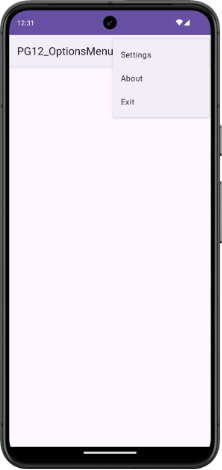
\includegraphics[width=0.4\textwidth]{Output_Screenshots/12_1.png} \quad 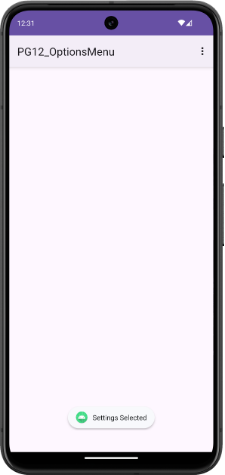
\includegraphics[width=0.4\textwidth]{Output_Screenshots/12_2.png} \end{center} \\
\end{longtable}
\endgroup

\newpage

%% ─── Program 13 ──────────────────────────────────────────────
\noindent\begingroup
\renewcommand{\arraystretch}{1.1}
\begin{longtable}{|p{0.94\textwidth}|}
\hline\endfirsthead\hline\endhead\hline\endfoot\hline\endlastfoot
\rule{0pt}{13pt}Program No: 13 \hfill Date: 29/06/2026 \\
\hline
\rule{0pt}{13pt}Program Title: Create an app that changes the background color of an activity using Context Menu. \\
\hline
\rule{0pt}{13pt}\textbf{MainActivity.java:} \\
\hline
{\ttfamily\small package\ com.example.context\_menu;} \\
\strut \\
{\ttfamily\small import\ android.graphics.Color;} \\
{\ttfamily\small import\ android.os.Bundle;} \\
{\ttfamily\small import\ androidx.appcompat.app.AppCompatActivity;} \\
{\ttfamily\small import\ android.view.ContextMenu;} \\
{\ttfamily\small import\ android.view.MenuInflater;} \\
{\ttfamily\small import\ android.view.MenuItem;} \\
{\ttfamily\small import\ android.view.View;} \\
{\ttfamily\small import\ android.widget.TextView;} \\
\strut \\
{\ttfamily\small public\ class\ MainActivity\ extends\ AppCompatActivity\ \{} \\
{\ttfamily\small \ \ \ \ View\ layout;} \\
{\ttfamily\small \ \ \ \ TextView\ tx1;} \\
\strut \\
{\ttfamily\small \ \ \ \ @Override} \\
{\ttfamily\small \ \ \ \ protected\ void\ onCreate(Bundle\ savedInstanceState)\ \{} \\
{\ttfamily\small \ \ \ \ \ \ \ \ super.onCreate(savedInstanceState);} \\
{\ttfamily\small \ \ \ \ \ \ \ \ setContentView(R.layout.activity\_main);} \\
{\ttfamily\small \ \ \ \ \ \ \ \ layout\ =\ findViewById(R.id.main);} \\
{\ttfamily\small \ \ \ \ \ \ \ \ tx1\ =\ findViewById(R.id.tx1);} \\
{\ttfamily\small \ \ \ \ \ \ \ \ registerForContextMenu(tx1);} \\
{\ttfamily\small \ \ \ \ \}} \\
\strut \\
{\ttfamily\small \ \ \ \ @Override} \\
{\ttfamily\small \ \ \ \ public\ void\ onCreateContextMenu(ContextMenu\ menu,\ View\ v,\ } \\
{\ttfamily\small \ \ \ \ \ \ \ \ \ \ \ \ \ \ \ \ \ \ \ \ \ \ \ \ \ \ \ \ \ \ \ \ \ \ \ \ ContextMenu.ContextMenuInfo\ menuinfo)\{} \\
{\ttfamily\small \ \ \ \ \ \ \ \ super.onCreateContextMenu(menu,\ v,\ menuinfo);} \\
{\ttfamily\small \ \ \ \ \ \ \ \ MenuInflater\ inflater\ =\ getMenuInflater();} \\
{\ttfamily\small \ \ \ \ \ \ \ \ inflater.inflate(R.menu.menu\_main,\ menu);} \\
{\ttfamily\small \ \ \ \ \}} \\
\strut \\
{\ttfamily\small \ \ \ \ public\ boolean\ onContextItemSelected(MenuItem\ item)\ \{} \\
{\ttfamily\small \ \ \ \ \ \ \ \ if\ (item.getItemId()\ ==\ R.id.red)\{} \\
{\ttfamily\small \ \ \ \ \ \ \ \ \ \ \ \ layout.setBackgroundColor(Color.RED);} \\
{\ttfamily\small \ \ \ \ \ \ \ \ \}} \\
{\ttfamily\small \ \ \ \ \ \ \ \ if\ (item.getItemId()\ ==\ R.id.blue)\ \{} \\
{\ttfamily\small \ \ \ \ \ \ \ \ \ \ \ \ layout.setBackgroundColor(Color.BLUE);} \\
{\ttfamily\small \ \ \ \ \ \ \ \ \}} \\
{\ttfamily\small \ \ \ \ \ \ \ \ if\ (item.getItemId()\ ==\ R.id.green)\ \{} \\
{\ttfamily\small \ \ \ \ \ \ \ \ \ \ \ \ layout.setBackgroundColor(Color.GREEN);} \\
{\ttfamily\small \ \ \ \ \ \ \ \ \}} \\
{\ttfamily\small \ \ \ \ \ \ \ \ if\ (item.getItemId()\ ==\ R.id.yellow)\ \{} \\
{\ttfamily\small \ \ \ \ \ \ \ \ \ \ \ \ layout.setBackgroundColor(Color.YELLOW);} \\
{\ttfamily\small \ \ \ \ \ \ \ \ \}} \\
{\ttfamily\small \ \ \ \ \ \ \ \ return\ false;} \\
{\ttfamily\small \ \ \ \ \}} \\
{\ttfamily\small \}} \\
\hline
\rule{0pt}{13pt}\textbf{activity\_main.xml:} \\
\hline
{\ttfamily\small \textless{}?xml\ version="1.0"\ encoding="utf-8"?\textgreater{}} \\
{\ttfamily\small \textless{}androidx.constraintlayout.widget.ConstraintLayout\ xmlns:android="http://schemas.android.com/apk/res/android"} \\
{\ttfamily\small \ \ \ \ xmlns:app="http://schemas.android.com/apk/res-auto"} \\
{\ttfamily\small \ \ \ \ xmlns:tools="http://schemas.android.com/tools"} \\
{\ttfamily\small \ \ \ \ android:id="@+id/main"} \\
{\ttfamily\small \ \ \ \ android:layout\_width="match\_parent"} \\
{\ttfamily\small \ \ \ \ android:layout\_height="match\_parent"} \\
{\ttfamily\small \ \ \ \ tools:context=".MainActivity"\textgreater{}} \\
\strut \\
{\ttfamily\small \ \ \ \ \textless{}TextView} \\
{\ttfamily\small \ \ \ \ \ \ \ \ android:id="@+id/tx1"} \\
{\ttfamily\small \ \ \ \ \ \ \ \ android:layout\_width="90dp"} \\
{\ttfamily\small \ \ \ \ \ \ \ \ android:layout\_height="30dp"} \\
{\ttfamily\small \ \ \ \ \ \ \ \ android:text="Hello\ World!"} \\
{\ttfamily\small \ \ \ \ \ \ \ \ app:layout\_constraintBottom\_toBottomOf="parent"} \\
{\ttfamily\small \ \ \ \ \ \ \ \ app:layout\_constraintEnd\_toEndOf="parent"} \\
{\ttfamily\small \ \ \ \ \ \ \ \ app:layout\_constraintHorizontal\_bias="0.454"} \\
{\ttfamily\small \ \ \ \ \ \ \ \ app:layout\_constraintStart\_toStartOf="parent"} \\
{\ttfamily\small \ \ \ \ \ \ \ \ app:layout\_constraintTop\_toTopOf="parent"} \\
{\ttfamily\small \ \ \ \ \ \ \ \ app:layout\_constraintVertical\_bias="0.499"\ /\textgreater{}} \\
\strut \\
{\ttfamily\small \textless{}/androidx.constraintlayout.widget.ConstraintLayout\textgreater{}} \\
\hline
\rule{0pt}{13pt}\textbf{menu.xml:} \\
\hline
{\ttfamily\small \textless{}?xml\ version="1.0"\ encoding="utf-8"?\textgreater{}} \\
{\ttfamily\small \textless{}menu\ xmlns:app="http://schemas.android.com/apk/res-auto"} \\
{\ttfamily\small \ \ \ \ xmlns:android="http://schemas.android.com/apk/res/android"\textgreater{}} \\
{\ttfamily\small \ \ \ \ \textless{}item} \\
{\ttfamily\small \ \ \ \ \ \ \ \ android:id="@+id/red"} \\
{\ttfamily\small \ \ \ \ \ \ \ \ android:title="RED"\ /\textgreater{}} \\
{\ttfamily\small \ \ \ \ \textless{}item} \\
{\ttfamily\small \ \ \ \ \ \ \ \ android:id="@+id/blue"} \\
{\ttfamily\small \ \ \ \ \ \ \ \ android:title="BLUE"\ /\textgreater{}} \\
{\ttfamily\small \ \ \ \ \textless{}item} \\
{\ttfamily\small \ \ \ \ \ \ \ \ android:id="@+id/green"} \\
{\ttfamily\small \ \ \ \ \ \ \ \ android:title="GREEN"\ /\textgreater{}} \\
{\ttfamily\small \ \ \ \ \textless{}item} \\
{\ttfamily\small \ \ \ \ \ \ \ \ android:id="@+id/yellow"} \\
{\ttfamily\small \ \ \ \ \ \ \ \ android:title="YELLOW"\ /\textgreater{}} \\
{\ttfamily\small \textless{}/menu\textgreater{}} \\
\hline
Output: \newline \begin{center} 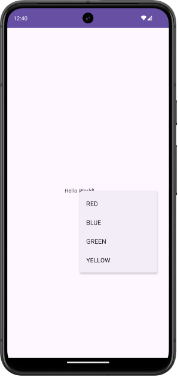
\includegraphics[width=0.4\textwidth]{Output_Screenshots/13_1.png} \quad 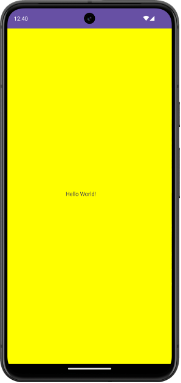
\includegraphics[width=0.4\textwidth]{Output_Screenshots/13_2.png} \end{center} \\
\end{longtable}
\endgroup

\newpage

%% ─── Program 14 ──────────────────────────────────────────────
\noindent\begingroup
\renewcommand{\arraystretch}{1.1}
\begin{longtable}{|p{0.94\textwidth}|}
\hline\endfirsthead\hline\endhead\hline\endfoot\hline\endlastfoot
\rule{0pt}{13pt}Program No: 14 \hfill Date: 29/06/2026 \\
\hline
\rule{0pt}{13pt}Program Title: Create an app to demonstrate how radiobuttons and checkboxes can be used in android. \\
\hline
\rule{0pt}{13pt}\textbf{MainActivity.java:} \\
\hline
{\ttfamily\small package\ com.example.radiocheckbox;} \\
\strut \\
{\ttfamily\small import\ android.os.Bundle;} \\
{\ttfamily\small import\ androidx.appcompat.app.AppCompatActivity;} \\
{\ttfamily\small import\ android.widget.Button;} \\
{\ttfamily\small import\ android.widget.RadioGroup;} \\
{\ttfamily\small import\ android.widget.RadioButton;} \\
{\ttfamily\small import\ android.widget.CheckBox;} \\
{\ttfamily\small import\ android.widget.Toast;} \\
\strut \\
{\ttfamily\small public\ class\ MainActivity\ extends\ AppCompatActivity\ \{} \\
{\ttfamily\small \ \ \ \ RadioGroup\ gender;} \\
{\ttfamily\small \ \ \ \ CheckBox\ ten,\ twelve,\ UG,\ PG;} \\
{\ttfamily\small \ \ \ \ Button\ submit;} \\
\strut \\
{\ttfamily\small \ \ \ \ @Override} \\
{\ttfamily\small \ \ \ \ protected\ void\ onCreate(Bundle\ savedInstanceState)\ \{} \\
{\ttfamily\small \ \ \ \ \ \ \ \ super.onCreate(savedInstanceState);} \\
{\ttfamily\small \ \ \ \ \ \ \ \ setContentView(R.layout.activity\_main);} \\
\strut \\
{\ttfamily\small \ \ \ \ \ \ \ \ gender\ =\ findViewById(R.id.gender);} \\
{\ttfamily\small \ \ \ \ \ \ \ \ ten\ =\ findViewById(R.id.ten);} \\
{\ttfamily\small \ \ \ \ \ \ \ \ twelve\ =\ findViewById(R.id.twelve);} \\
{\ttfamily\small \ \ \ \ \ \ \ \ UG\ =\ findViewById(R.id.UG);} \\
{\ttfamily\small \ \ \ \ \ \ \ \ PG\ =\ findViewById(R.id.PG);} \\
{\ttfamily\small \ \ \ \ \ \ \ \ submit\ =\ findViewById(R.id.submit);} \\
\strut \\
{\ttfamily\small \ \ \ \ \ \ \ \ submit.setOnClickListener(v\ -\textgreater{}\{} \\
{\ttfamily\small \ \ \ \ \ \ \ \ \ \ \ \ int\ selectedId\ =\ gender.getCheckedRadioButtonId();} \\
{\ttfamily\small \ \ \ \ \ \ \ \ \ \ \ \ RadioButton\ rb\ =\ findViewById(selectedId);} \\
{\ttfamily\small \ \ \ \ \ \ \ \ \ \ \ \ String\ gen\ =\ rb.getText().toString();} \\
{\ttfamily\small \ \ \ \ \ \ \ \ \ \ \ \ StringBuilder\ education\ =\ new\ StringBuilder();} \\
\strut \\
{\ttfamily\small \ \ \ \ \ \ \ \ \ \ \ \ if\ (ten.isChecked())\ education.append("Tenth\ ");} \\
{\ttfamily\small \ \ \ \ \ \ \ \ \ \ \ \ if\ (twelve.isChecked())\ education.append("Plus\ Two\ ");} \\
{\ttfamily\small \ \ \ \ \ \ \ \ \ \ \ \ if\ (UG.isChecked())\ education.append("Undergraduate\ ");} \\
{\ttfamily\small \ \ \ \ \ \ \ \ \ \ \ \ if\ (PG.isChecked())\ education.append("Postgraduate\ ");} \\
\strut \\
{\ttfamily\small \ \ \ \ \ \ \ \ \ \ \ \ Toast.makeText(this,\ gen\ +\ "\ |\ "\ +\ education,\ } \\
{\ttfamily\small \ \ \ \ \ \ \ \ \ \ \ \ \ \ \ \ \ \ \ \ \ \ \ \ \ \ \ Toast.LENGTH\_LONG).show();} \\
{\ttfamily\small \ \ \ \ \ \ \ \ \});} \\
{\ttfamily\small \ \ \ \ \}} \\
{\ttfamily\small \}} \\
\hline
\rule{0pt}{13pt}\textbf{activity\_main.xml:} \\
\hline
{\ttfamily\small \textless{}?xml\ version="1.0"\ encoding="utf-8"?\textgreater{}} \\
{\ttfamily\small \textless{}androidx.constraintlayout.widget.ConstraintLayout\ xmlns:android="http://schemas.android.com/apk/res/android"} \\
{\ttfamily\small \ \ \ \ xmlns:app="http://schemas.android.com/apk/res-auto"} \\
{\ttfamily\small \ \ \ \ xmlns:tools="http://schemas.android.com/tools"} \\
{\ttfamily\small \ \ \ \ android:id="@+id/main"} \\
{\ttfamily\small \ \ \ \ android:layout\_width="match\_parent"} \\
{\ttfamily\small \ \ \ \ android:layout\_height="match\_parent"} \\
{\ttfamily\small \ \ \ \ android:background="\#FB9E9E"} \\
{\ttfamily\small \ \ \ \ tools:context=".MainActivity"\textgreater{}} \\
\strut \\
{\ttfamily\small \ \ \ \ \textless{}TextView} \\
{\ttfamily\small \ \ \ \ \ \ \ \ android:id="@+id/textView4"} \\
{\ttfamily\small \ \ \ \ \ \ \ \ android:layout\_width="82dp"} \\
{\ttfamily\small \ \ \ \ \ \ \ \ android:layout\_height="23dp"} \\
{\ttfamily\small \ \ \ \ \ \ \ \ android:text="Gender:\ "} \\
{\ttfamily\small \ \ \ \ \ \ \ \ app:layout\_constraintBottom\_toBottomOf="parent"} \\
{\ttfamily\small \ \ \ \ \ \ \ \ app:layout\_constraintEnd\_toEndOf="parent"} \\
{\ttfamily\small \ \ \ \ \ \ \ \ app:layout\_constraintHorizontal\_bias="0.124"} \\
{\ttfamily\small \ \ \ \ \ \ \ \ app:layout\_constraintStart\_toStartOf="parent"} \\
{\ttfamily\small \ \ \ \ \ \ \ \ app:layout\_constraintTop\_toTopOf="parent"} \\
{\ttfamily\small \ \ \ \ \ \ \ \ app:layout\_constraintVertical\_bias="0.114"\ /\textgreater{}} \\
\strut \\
{\ttfamily\small \ \ \ \ \textless{}RadioGroup} \\
{\ttfamily\small \ \ \ \ \ \ \ \ android:id="@+id/gender"} \\
{\ttfamily\small \ \ \ \ \ \ \ \ android:layout\_width="247dp"} \\
{\ttfamily\small \ \ \ \ \ \ \ \ android:layout\_height="143dp"} \\
{\ttfamily\small \ \ \ \ \ \ \ \ app:layout\_constraintBottom\_toBottomOf="parent"} \\
{\ttfamily\small \ \ \ \ \ \ \ \ app:layout\_constraintEnd\_toEndOf="parent"} \\
{\ttfamily\small \ \ \ \ \ \ \ \ app:layout\_constraintHorizontal\_bias="0.25"} \\
{\ttfamily\small \ \ \ \ \ \ \ \ app:layout\_constraintStart\_toStartOf="parent"} \\
{\ttfamily\small \ \ \ \ \ \ \ \ app:layout\_constraintTop\_toTopOf="parent"} \\
{\ttfamily\small \ \ \ \ \ \ \ \ app:layout\_constraintVertical\_bias="0.205"\textgreater{}} \\
{\ttfamily\small \ \ \ \ \ \ \ \ \textless{}RadioButton} \\
{\ttfamily\small \ \ \ \ \ \ \ \ \ \ \ \ android:id="@+id/male"} \\
{\ttfamily\small \ \ \ \ \ \ \ \ \ \ \ \ android:layout\_width="match\_parent"} \\
{\ttfamily\small \ \ \ \ \ \ \ \ \ \ \ \ android:layout\_height="wrap\_content"} \\
{\ttfamily\small \ \ \ \ \ \ \ \ \ \ \ \ android:text="Male"\ /\textgreater{}} \\
{\ttfamily\small \ \ \ \ \ \ \ \ \textless{}RadioButton} \\
{\ttfamily\small \ \ \ \ \ \ \ \ \ \ \ \ android:id="@+id/female"} \\
{\ttfamily\small \ \ \ \ \ \ \ \ \ \ \ \ android:layout\_width="match\_parent"} \\
{\ttfamily\small \ \ \ \ \ \ \ \ \ \ \ \ android:layout\_height="wrap\_content"} \\
{\ttfamily\small \ \ \ \ \ \ \ \ \ \ \ \ android:text="Female"\ /\textgreater{}} \\
{\ttfamily\small \ \ \ \ \ \ \ \ \textless{}RadioButton} \\
{\ttfamily\small \ \ \ \ \ \ \ \ \ \ \ \ android:id="@+id/tg"} \\
{\ttfamily\small \ \ \ \ \ \ \ \ \ \ \ \ android:layout\_width="match\_parent"} \\
{\ttfamily\small \ \ \ \ \ \ \ \ \ \ \ \ android:layout\_height="wrap\_content"} \\
{\ttfamily\small \ \ \ \ \ \ \ \ \ \ \ \ android:text="TG"\ /\textgreater{}} \\
{\ttfamily\small \ \ \ \ \textless{}/RadioGroup\textgreater{}} \\
\strut \\
{\ttfamily\small \ \ \ \ \textless{}CheckBox} \\
{\ttfamily\small \ \ \ \ \ \ \ \ android:id="@+id/ten"} \\
{\ttfamily\small \ \ \ \ \ \ \ \ android:layout\_width="134dp"} \\
{\ttfamily\small \ \ \ \ \ \ \ \ android:layout\_height="43dp"} \\
{\ttfamily\small \ \ \ \ \ \ \ \ android:text="X"} \\
{\ttfamily\small \ \ \ \ \ \ \ \ app:layout\_constraintBottom\_toBottomOf="parent"} \\
{\ttfamily\small \ \ \ \ \ \ \ \ app:layout\_constraintEnd\_toEndOf="parent"} \\
{\ttfamily\small \ \ \ \ \ \ \ \ app:layout\_constraintHorizontal\_bias="0.155"} \\
{\ttfamily\small \ \ \ \ \ \ \ \ app:layout\_constraintStart\_toStartOf="parent"} \\
{\ttfamily\small \ \ \ \ \ \ \ \ app:layout\_constraintTop\_toTopOf="parent"} \\
{\ttfamily\small \ \ \ \ \ \ \ \ app:layout\_constraintVertical\_bias="0.527"\ /\textgreater{}} \\
\strut \\
{\ttfamily\small \ \ \ \ \textless{}CheckBox} \\
{\ttfamily\small \ \ \ \ \ \ \ \ android:id="@+id/UG"} \\
{\ttfamily\small \ \ \ \ \ \ \ \ android:layout\_width="133dp"} \\
{\ttfamily\small \ \ \ \ \ \ \ \ android:layout\_height="48dp"} \\
{\ttfamily\small \ \ \ \ \ \ \ \ android:text="UG"} \\
{\ttfamily\small \ \ \ \ \ \ \ \ app:layout\_constraintBottom\_toBottomOf="parent"} \\
{\ttfamily\small \ \ \ \ \ \ \ \ app:layout\_constraintEnd\_toEndOf="parent"} \\
{\ttfamily\small \ \ \ \ \ \ \ \ app:layout\_constraintHorizontal\_bias="0.154"} \\
{\ttfamily\small \ \ \ \ \ \ \ \ app:layout\_constraintStart\_toStartOf="parent"} \\
{\ttfamily\small \ \ \ \ \ \ \ \ app:layout\_constraintTop\_toTopOf="parent"} \\
{\ttfamily\small \ \ \ \ \ \ \ \ app:layout\_constraintVertical\_bias="0.71"\ /\textgreater{}} \\
\strut \\
{\ttfamily\small \ \ \ \ \textless{}CheckBox} \\
{\ttfamily\small \ \ \ \ \ \ \ \ android:id="@+id/twelve"} \\
{\ttfamily\small \ \ \ \ \ \ \ \ android:layout\_width="134dp"} \\
{\ttfamily\small \ \ \ \ \ \ \ \ android:layout\_height="48dp"} \\
{\ttfamily\small \ \ \ \ \ \ \ \ android:text="XII"} \\
{\ttfamily\small \ \ \ \ \ \ \ \ app:layout\_constraintBottom\_toBottomOf="parent"} \\
{\ttfamily\small \ \ \ \ \ \ \ \ app:layout\_constraintEnd\_toEndOf="parent"} \\
{\ttfamily\small \ \ \ \ \ \ \ \ app:layout\_constraintHorizontal\_bias="0.158"} \\
{\ttfamily\small \ \ \ \ \ \ \ \ app:layout\_constraintStart\_toStartOf="parent"} \\
{\ttfamily\small \ \ \ \ \ \ \ \ app:layout\_constraintTop\_toTopOf="parent"} \\
{\ttfamily\small \ \ \ \ \ \ \ \ app:layout\_constraintVertical\_bias="0.619"\ /\textgreater{}} \\
\strut \\
{\ttfamily\small \ \ \ \ \textless{}Button} \\
{\ttfamily\small \ \ \ \ \ \ \ \ android:id="@+id/submit"} \\
{\ttfamily\small \ \ \ \ \ \ \ \ android:layout\_width="wrap\_content"} \\
{\ttfamily\small \ \ \ \ \ \ \ \ android:layout\_height="wrap\_content"} \\
{\ttfamily\small \ \ \ \ \ \ \ \ android:text="Submit"} \\
{\ttfamily\small \ \ \ \ \ \ \ \ app:layout\_constraintBottom\_toBottomOf="parent"} \\
{\ttfamily\small \ \ \ \ \ \ \ \ app:layout\_constraintEnd\_toEndOf="parent"} \\
{\ttfamily\small \ \ \ \ \ \ \ \ app:layout\_constraintHorizontal\_bias="0.468"} \\
{\ttfamily\small \ \ \ \ \ \ \ \ app:layout\_constraintStart\_toStartOf="parent"} \\
{\ttfamily\small \ \ \ \ \ \ \ \ app:layout\_constraintTop\_toTopOf="parent"} \\
{\ttfamily\small \ \ \ \ \ \ \ \ app:layout\_constraintVertical\_bias="0.915"\ /\textgreater{}} \\
\strut \\
{\ttfamily\small \ \ \ \ \textless{}TextView} \\
{\ttfamily\small \ \ \ \ \ \ \ \ android:id="@+id/textView"} \\
{\ttfamily\small \ \ \ \ \ \ \ \ android:layout\_width="90dp"} \\
{\ttfamily\small \ \ \ \ \ \ \ \ android:layout\_height="22dp"} \\
{\ttfamily\small \ \ \ \ \ \ \ \ android:text="Qualification"} \\
{\ttfamily\small \ \ \ \ \ \ \ \ app:layout\_constraintBottom\_toBottomOf="parent"} \\
{\ttfamily\small \ \ \ \ \ \ \ \ app:layout\_constraintEnd\_toEndOf="parent"} \\
{\ttfamily\small \ \ \ \ \ \ \ \ app:layout\_constraintHorizontal\_bias="0.13"} \\
{\ttfamily\small \ \ \ \ \ \ \ \ app:layout\_constraintStart\_toStartOf="parent"} \\
{\ttfamily\small \ \ \ \ \ \ \ \ app:layout\_constraintTop\_toTopOf="parent"} \\
{\ttfamily\small \ \ \ \ \ \ \ \ app:layout\_constraintVertical\_bias="0.452"\ /\textgreater{}} \\
\strut \\
{\ttfamily\small \ \ \ \ \textless{}CheckBox} \\
{\ttfamily\small \ \ \ \ \ \ \ \ android:id="@+id/PG"} \\
{\ttfamily\small \ \ \ \ \ \ \ \ android:layout\_width="133dp"} \\
{\ttfamily\small \ \ \ \ \ \ \ \ android:layout\_height="48dp"} \\
{\ttfamily\small \ \ \ \ \ \ \ \ android:text="PG"} \\
{\ttfamily\small \ \ \ \ \ \ \ \ app:layout\_constraintBottom\_toBottomOf="parent"} \\
{\ttfamily\small \ \ \ \ \ \ \ \ app:layout\_constraintEnd\_toEndOf="parent"} \\
{\ttfamily\small \ \ \ \ \ \ \ \ app:layout\_constraintHorizontal\_bias="0.154"} \\
{\ttfamily\small \ \ \ \ \ \ \ \ app:layout\_constraintStart\_toStartOf="parent"} \\
{\ttfamily\small \ \ \ \ \ \ \ \ app:layout\_constraintTop\_toTopOf="parent"} \\
{\ttfamily\small \ \ \ \ \ \ \ \ app:layout\_constraintVertical\_bias="0.808"\ /\textgreater{}} \\
\strut \\
{\ttfamily\small \textless{}/androidx.constraintlayout.widget.ConstraintLayout\textgreater{}} \\
\hline
Output: \newline \begin{center} 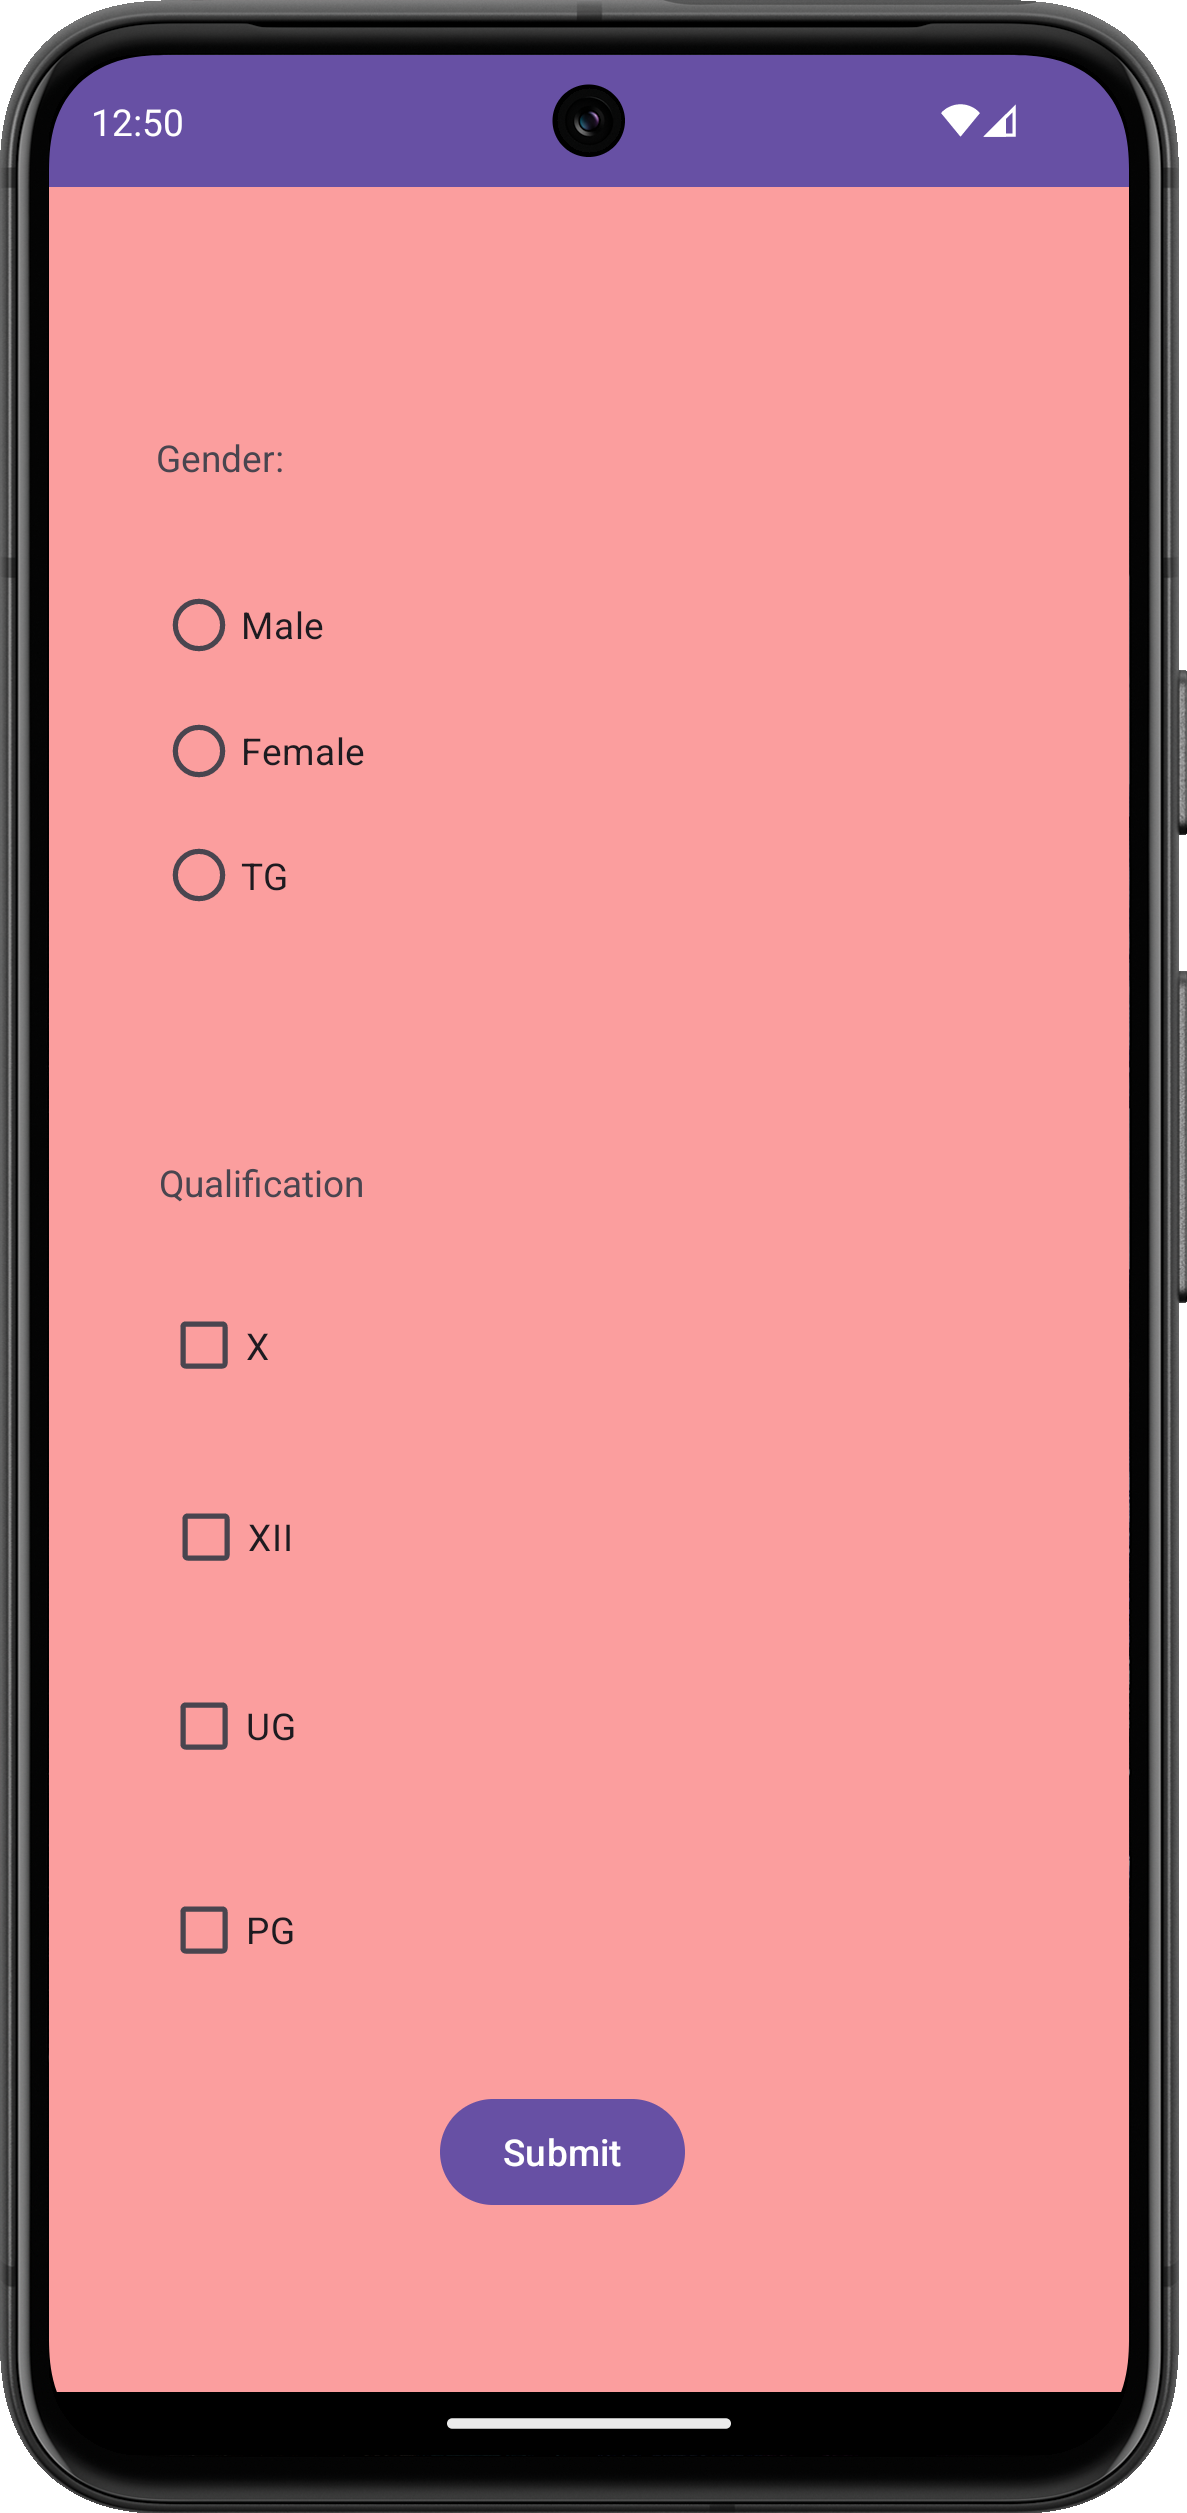
\includegraphics[width=0.4\textwidth]{Output_Screenshots/14_1.png} \quad 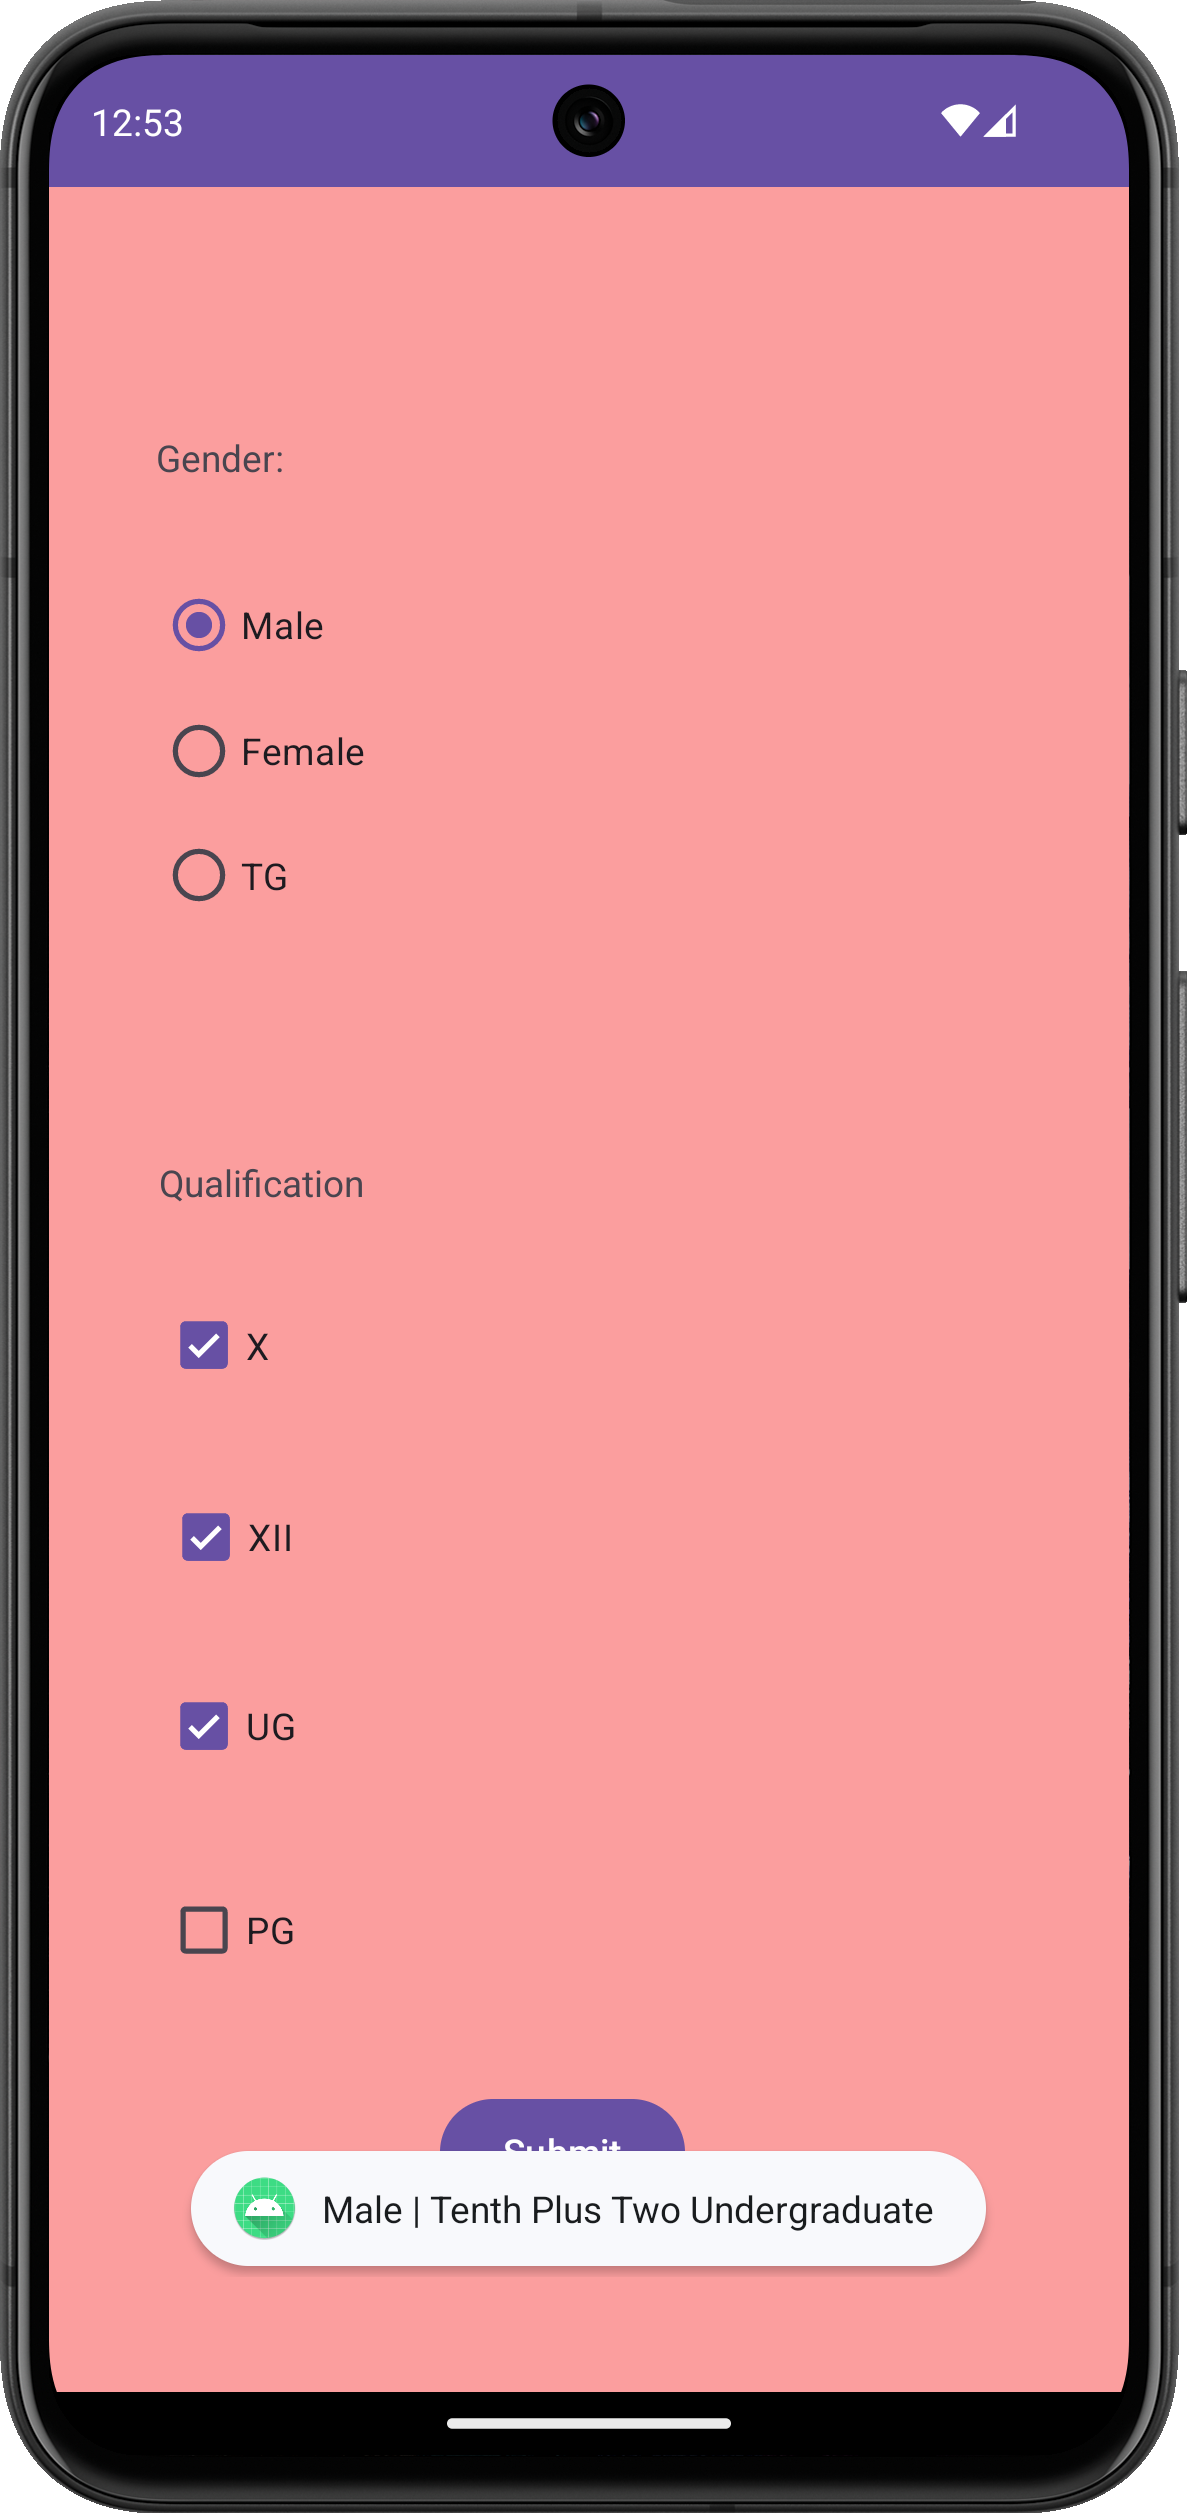
\includegraphics[width=0.4\textwidth]{Output_Screenshots/14_2.png} \end{center} \\
\end{longtable}
\endgroup

\newpage

%% ─── Program 15 ──────────────────────────────────────────────
\noindent\begingroup
\renewcommand{\arraystretch}{1.1}
\begin{longtable}{|p{0.94\textwidth}|}
\hline\endfirsthead\hline\endhead\hline\endfoot\hline\endlastfoot
\rule{0pt}{13pt}Program No: 15 \hfill Date: 29/06/2026 \\
\hline
\rule{0pt}{13pt}Program Title: Create an app that launches a new activity on a button click \\
\hline
\rule{0pt}{13pt}\textbf{MainActivity.java:} \\
\hline
{\ttfamily\small package\ com.example.a2screen\_welcome;} \\
{\ttfamily\small import\ android.content.Intent;} \\
{\ttfamily\small import\ android.os.Bundle;} \\
{\ttfamily\small import\ androidx.appcompat.app.AppCompatActivity;} \\
{\ttfamily\small import\ android.widget.Button;} \\
\strut \\
{\ttfamily\small public\ class\ MainActivity\ extends\ AppCompatActivity\ \{} \\
{\ttfamily\small \ \ \ \ @Override} \\
{\ttfamily\small \ \ \ \ protected\ void\ onCreate(Bundle\ savedInstanceState)\ \{} \\
{\ttfamily\small \ \ \ \ \ \ \ \ super.onCreate(savedInstanceState);} \\
{\ttfamily\small \ \ \ \ \ \ \ \ setContentView(R.layout.activity\_main);} \\
{\ttfamily\small \ \ \ \ \ \ \ \ Button\ btn\ =\ findViewById(R.id.button);} \\
{\ttfamily\small \ \ \ \ \ \ \ \ btn.setOnClickListener(v-\textgreater{}\ \{} \\
{\ttfamily\small \ \ \ \ \ \ \ \ \ \ \ \ Intent\ intent\ =\ new\ Intent(MainActivity.this,\ } \\
{\ttfamily\small \ \ \ \ \ \ \ \ \ \ \ \ \ \ \ \ \ \ \ \ \ \ \ \ \ \ \ \ \ \ \ \ \ \ \ \ \ \ \ SecondaryActivity.class);} \\
{\ttfamily\small \ \ \ \ \ \ \ \ \ \ \ \ startActivity(intent);} \\
{\ttfamily\small \ \ \ \ \ \ \ \ \});} \\
{\ttfamily\small \ \ \ \ \}} \\
{\ttfamily\small \}} \\
\hline
\rule{0pt}{13pt}\textbf{SecondaryActivity.java:} \\
\hline
{\ttfamily\small package\ com.example.a2screen\_welcome;} \\
{\ttfamily\small import\ android.os.Bundle;} \\
{\ttfamily\small import\ androidx.appcompat.app.AppCompatActivity;} \\
\strut \\
{\ttfamily\small public\ class\ SecondaryActivity\ extends\ AppCompatActivity\ \{} \\
{\ttfamily\small \ \ \ \ @Override} \\
{\ttfamily\small \ \ \ \ protected\ void\ onCreate(Bundle\ savedInstanceState)\ \{} \\
{\ttfamily\small \ \ \ \ \ \ \ \ super.onCreate(savedInstanceState);} \\
{\ttfamily\small \ \ \ \ \ \ \ \ setContentView(R.layout.activity\_secondary);} \\
{\ttfamily\small \ \ \ \ \}} \\
{\ttfamily\small \}} \\
\hline
\rule{0pt}{13pt}\textbf{activity\_main.xml:} \\
\hline
{\ttfamily\small \textless{}?xml\ version="1.0"\ encoding="utf-8"?\textgreater{}} \\
{\ttfamily\small \textless{}androidx.constraintlayout.widget.ConstraintLayout\ xmlns:android="http://schemas.android.com/apk/res/android"} \\
{\ttfamily\small \ \ \ \ xmlns:app="http://schemas.android.com/apk/res-auto"} \\
{\ttfamily\small \ \ \ \ xmlns:tools="http://schemas.android.com/tools"} \\
{\ttfamily\small \ \ \ \ android:id="@+id/main"} \\
{\ttfamily\small \ \ \ \ android:layout\_width="match\_parent"} \\
{\ttfamily\small \ \ \ \ android:layout\_height="match\_parent"} \\
{\ttfamily\small \ \ \ \ tools:context=".MainActivity"\textgreater{}} \\
\strut \\
{\ttfamily\small \ \ \ \ \textless{}Button} \\
{\ttfamily\small \ \ \ \ \ \ \ \ android:id="@+id/button"} \\
{\ttfamily\small \ \ \ \ \ \ \ \ android:layout\_width="172dp"} \\
{\ttfamily\small \ \ \ \ \ \ \ \ android:layout\_height="74dp"} \\
{\ttfamily\small \ \ \ \ \ \ \ \ android:text="Go\ to\ Next\ Page"} \\
{\ttfamily\small \ \ \ \ \ \ \ \ app:layout\_constraintBottom\_toBottomOf="parent"} \\
{\ttfamily\small \ \ \ \ \ \ \ \ app:layout\_constraintEnd\_toEndOf="parent"} \\
{\ttfamily\small \ \ \ \ \ \ \ \ app:layout\_constraintHorizontal\_bias="0.498"} \\
{\ttfamily\small \ \ \ \ \ \ \ \ app:layout\_constraintStart\_toStartOf="parent"} \\
{\ttfamily\small \ \ \ \ \ \ \ \ app:layout\_constraintTop\_toTopOf="parent"} \\
{\ttfamily\small \ \ \ \ \ \ \ \ app:layout\_constraintVertical\_bias="0.558"\ /\textgreater{}} \\
{\ttfamily\small \textless{}/androidx.constraintlayout.widget.ConstraintLayout\textgreater{}} \\
\hline
\rule{0pt}{13pt}\textbf{activity\_secondary.xml:} \\
\hline
{\ttfamily\small \textless{}?xml\ version="1.0"\ encoding="utf-8"?\textgreater{}} \\
{\ttfamily\small \textless{}androidx.constraintlayout.widget.ConstraintLayout\ xmlns:android="http://schemas.android.com/apk/res/android"} \\
{\ttfamily\small \ \ \ \ xmlns:app="http://schemas.android.com/apk/res-auto"} \\
{\ttfamily\small \ \ \ \ xmlns:tools="http://schemas.android.com/tools"} \\
{\ttfamily\small \ \ \ \ android:id="@+id/main"} \\
{\ttfamily\small \ \ \ \ android:layout\_width="match\_parent"} \\
{\ttfamily\small \ \ \ \ android:layout\_height="match\_parent"} \\
{\ttfamily\small \ \ \ \ android:background="\#EF9696"} \\
{\ttfamily\small \ \ \ \ tools:context=".SecondaryActivity"\textgreater{}} \\
\strut \\
{\ttfamily\small \ \ \ \ \textless{}TextView} \\
{\ttfamily\small \ \ \ \ \ \ \ \ android:id="@+id/textView"} \\
{\ttfamily\small \ \ \ \ \ \ \ \ android:layout\_width="66dp"} \\
{\ttfamily\small \ \ \ \ \ \ \ \ android:layout\_height="28dp"} \\
{\ttfamily\small \ \ \ \ \ \ \ \ android:text="Welcome"} \\
{\ttfamily\small \ \ \ \ \ \ \ \ app:layout\_constraintBottom\_toBottomOf="parent"} \\
{\ttfamily\small \ \ \ \ \ \ \ \ app:layout\_constraintEnd\_toEndOf="parent"} \\
{\ttfamily\small \ \ \ \ \ \ \ \ app:layout\_constraintStart\_toStartOf="parent"} \\
{\ttfamily\small \ \ \ \ \ \ \ \ app:layout\_constraintTop\_toTopOf="parent"\ /\textgreater{}} \\
{\ttfamily\small \textless{}/androidx.constraintlayout.widget.ConstraintLayout\textgreater{}} \\
\hline
Output: \newline \begin{center} 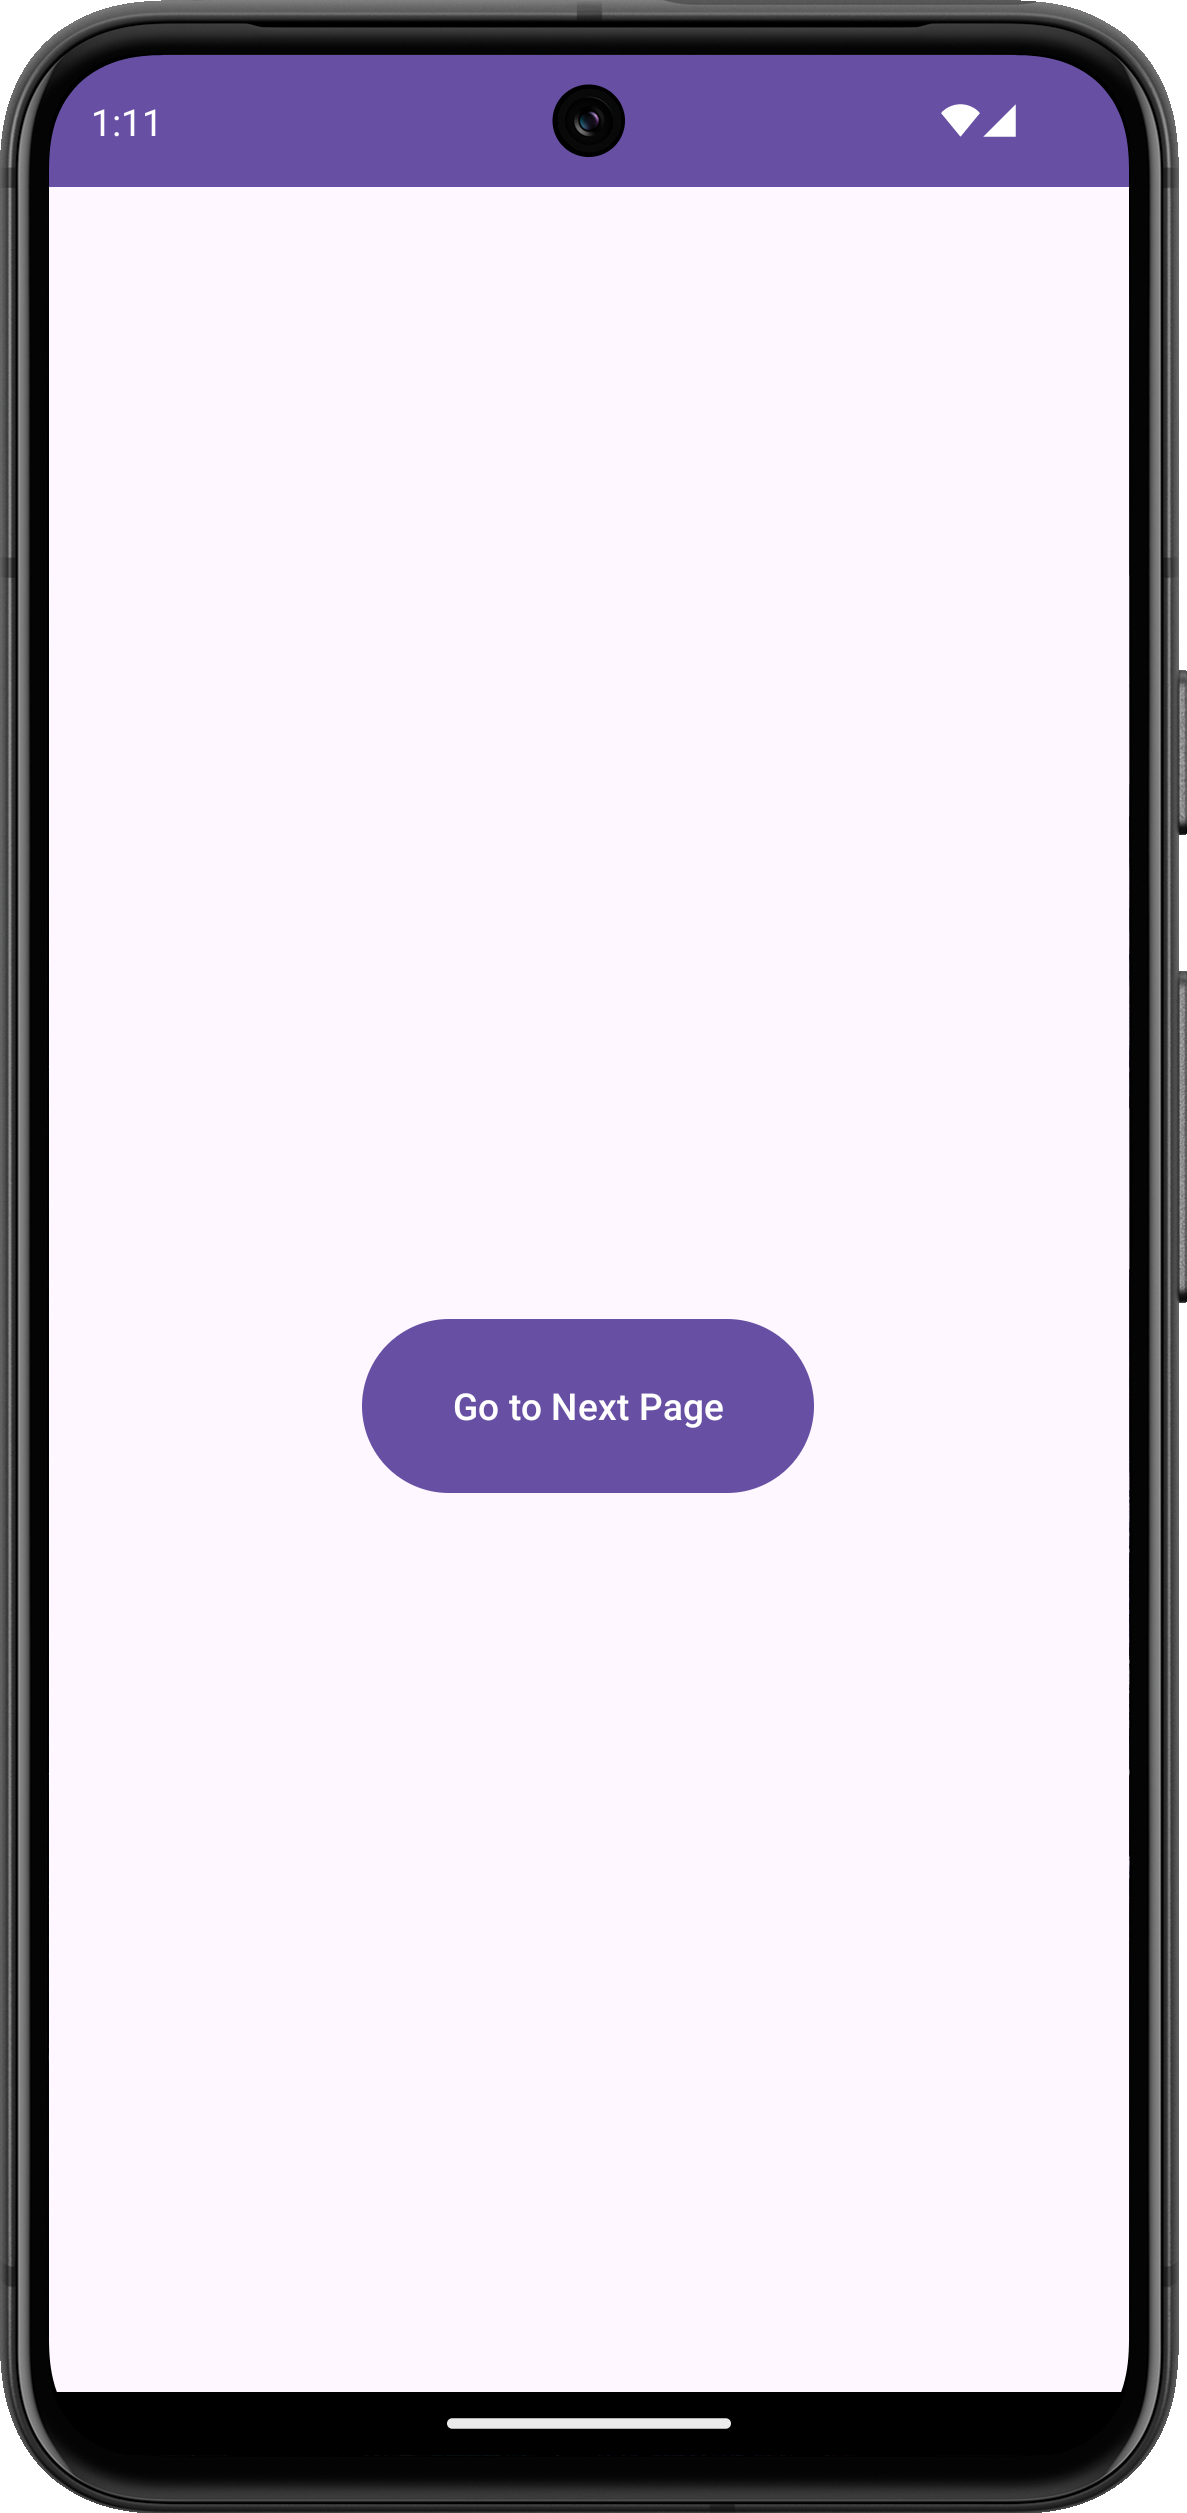
\includegraphics[width=0.4\textwidth]{Output_Screenshots/15_1.png} \quad 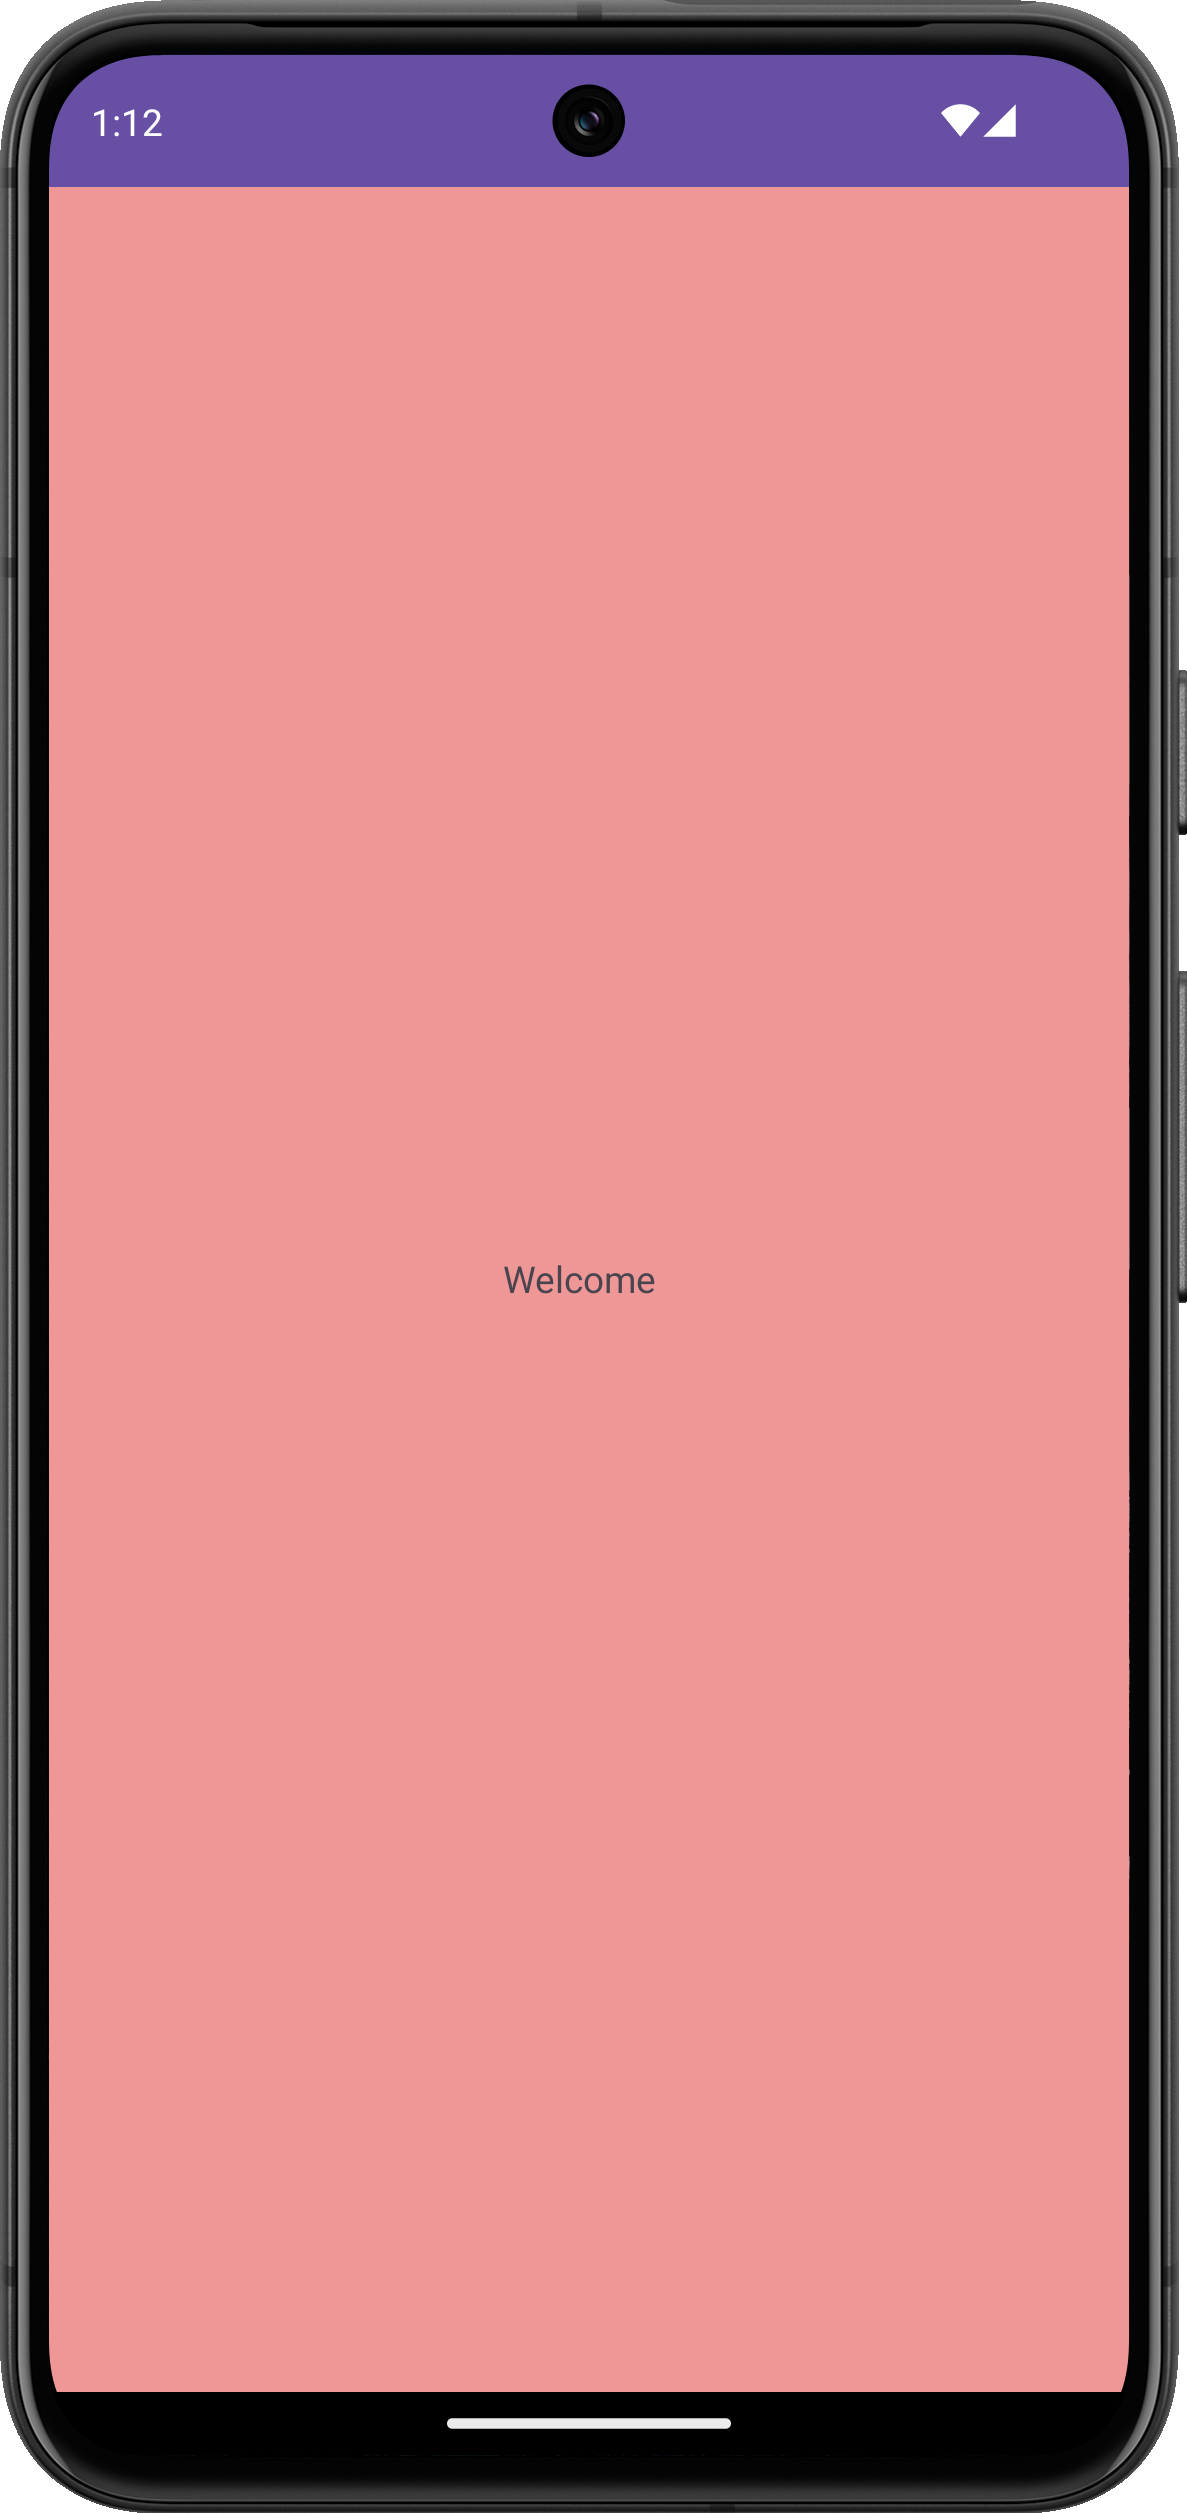
\includegraphics[width=0.4\textwidth]{Output_Screenshots/15_2.png} \end{center} \\
\end{longtable}
\endgroup

\newpage

%% ─── Program 16 ──────────────────────────────────────────────
\noindent\begingroup
\renewcommand{\arraystretch}{1.1}
\begin{longtable}{|p{0.94\textwidth}|}
\hline\endfirsthead\hline\endhead\hline\endfoot\hline\endlastfoot
\rule{0pt}{13pt}Program No: 16 \hfill Date: 29/06/2026 \\
\hline
\rule{0pt}{13pt}Program Title: Create an app that launches a new activity on a button click to display student details with checkbox and radio buttons. \\
\hline
\rule{0pt}{13pt}\textbf{MainActivity.java:} \\
\hline
{\ttfamily\small package\ com.example.pg16\_studentdetails;} \\
\strut \\
{\ttfamily\small import\ android.content.Intent;} \\
{\ttfamily\small import\ android.os.Bundle;} \\
{\ttfamily\small import\ androidx.appcompat.app.AppCompatActivity;} \\
{\ttfamily\small import\ android.widget.Button;} \\
{\ttfamily\small import\ android.widget.CheckBox;} \\
{\ttfamily\small import\ android.widget.EditText;} \\
{\ttfamily\small import\ android.widget.RadioButton;} \\
{\ttfamily\small import\ android.widget.RadioGroup;} \\
\strut \\
{\ttfamily\small public\ class\ MainActivity\ extends\ AppCompatActivity\ \{} \\
\strut \\
{\ttfamily\small \ \ \ \ @Override} \\
{\ttfamily\small \ \ \ \ protected\ void\ onCreate(Bundle\ savedInstanceState)\ \{} \\
{\ttfamily\small \ \ \ \ \ \ \ \ super.onCreate(savedInstanceState);} \\
{\ttfamily\small \ \ \ \ \ \ \ \ setContentView(R.layout.activity\_main);} \\
\strut \\
{\ttfamily\small \ \ \ \ \ \ \ \ Button\ submit\ =\ findViewById(R.id.submit);} \\
{\ttfamily\small \ \ \ \ \ \ \ \ EditText\ name\ =\ findViewById(R.id.name);} \\
{\ttfamily\small \ \ \ \ \ \ \ \ EditText\ mobile\ =\ findViewById(R.id.mobile);} \\
{\ttfamily\small \ \ \ \ \ \ \ \ RadioGroup\ department\ =\ findViewById(R.id.department);} \\
{\ttfamily\small \ \ \ \ \ \ \ \ RadioGroup\ gender\ =\ findViewById(R.id.gender);} \\
{\ttfamily\small \ \ \ \ \ \ \ \ CheckBox\ ai\ =\ findViewById(R.id.ai);} \\
{\ttfamily\small \ \ \ \ \ \ \ \ CheckBox\ cloud\ =\ findViewById(R.id.cloud);} \\
{\ttfamily\small \ \ \ \ \ \ \ \ CheckBox\ auto\ =\ findViewById(R.id.autocad);} \\
{\ttfamily\small \ \ \ \ \ \ \ \ CheckBox\ ship\ =\ findViewById(R.id.ship);} \\
\strut \\
{\ttfamily\small \ \ \ \ \ \ \ \ submit.setOnClickListener(v\ -\textgreater{}\ \{} \\
{\ttfamily\small \ \ \ \ \ \ \ \ \ \ \ \ int\ depId\ =\ department.getCheckedRadioButtonId();} \\
{\ttfamily\small \ \ \ \ \ \ \ \ \ \ \ \ RadioButton\ rdep\ =\ findViewById(depId);} \\
{\ttfamily\small \ \ \ \ \ \ \ \ \ \ \ \ int\ genId\ =\ gender.getCheckedRadioButtonId();} \\
{\ttfamily\small \ \ \ \ \ \ \ \ \ \ \ \ RadioButton\ rgen\ =\ findViewById(genId);} \\
{\ttfamily\small \ \ \ \ \ \ \ \ \ \ \ \ StringBuilder\ sb\ =\ new\ StringBuilder();} \\
\strut \\
{\ttfamily\small \ \ \ \ \ \ \ \ \ \ \ \ if\ (ai.isChecked())} \\
{\ttfamily\small \ \ \ \ \ \ \ \ \ \ \ \ \ \ \ \ sb.append("AI/ML\textbackslash{}n");} \\
\strut \\
{\ttfamily\small \ \ \ \ \ \ \ \ \ \ \ \ if\ (cloud.isChecked())} \\
{\ttfamily\small \ \ \ \ \ \ \ \ \ \ \ \ \ \ \ \ sb.append("Cloud\ Computing\textbackslash{}n");} \\
\strut \\
{\ttfamily\small \ \ \ \ \ \ \ \ \ \ \ \ if\ (auto.isChecked())} \\
{\ttfamily\small \ \ \ \ \ \ \ \ \ \ \ \ \ \ \ \ sb.append("AutoCAD\textbackslash{}n");} \\
\strut \\
{\ttfamily\small \ \ \ \ \ \ \ \ \ \ \ \ if\ (ship.isChecked())} \\
{\ttfamily\small \ \ \ \ \ \ \ \ \ \ \ \ \ \ \ \ sb.append("Ship\ Technology\textbackslash{}n");} \\
\strut \\
{\ttfamily\small \ \ \ \ \ \ \ \ \ \ \ \ Intent\ intent\ =\ new\ Intent(MainActivity.this,\ Details.class);} \\
{\ttfamily\small \ \ \ \ \ \ \ \ \ \ \ \ intent.putExtra("name",\ name.getText().toString());} \\
{\ttfamily\small \ \ \ \ \ \ \ \ \ \ \ \ intent.putExtra("mobile",\ mobile.getText().toString());} \\
{\ttfamily\small \ \ \ \ \ \ \ \ \ \ \ \ intent.putExtra("courses",\ sb.toString());} \\
{\ttfamily\small \ \ \ \ \ \ \ \ \ \ \ \ intent.putExtra("department",\ rdep.getText().toString());} \\
{\ttfamily\small \ \ \ \ \ \ \ \ \ \ \ \ intent.putExtra("gender",\ rgen.getText().toString());} \\
{\ttfamily\small \ \ \ \ \ \ \ \ \ \ \ \ startActivity(intent);} \\
{\ttfamily\small \ \ \ \ \ \ \ \ \});} \\
{\ttfamily\small \ \ \ \ \}} \\
{\ttfamily\small \}} \\
\hline
\rule{0pt}{13pt}\textbf{SecondaryActivity.java:} \\
\hline
{\ttfamily\small package\ com.example.pg16\_studentdetails;} \\
\strut \\
{\ttfamily\small import\ android.os.Bundle;} \\
{\ttfamily\small import\ androidx.appcompat.app.AppCompatActivity;} \\
{\ttfamily\small import\ android.widget.TextView;} \\
\strut \\
{\ttfamily\small public\ class\ Details\ extends\ AppCompatActivity\ \{} \\
\strut \\
{\ttfamily\small \ \ \ \ @Override} \\
{\ttfamily\small \ \ \ \ protected\ void\ onCreate(Bundle\ savedInstanceState)\ \{} \\
{\ttfamily\small \ \ \ \ \ \ \ \ super.onCreate(savedInstanceState);} \\
{\ttfamily\small \ \ \ \ \ \ \ \ setContentView(R.layout.activity\_details);} \\
\strut \\
{\ttfamily\small \ \ \ \ \ \ \ \ String\ name\ =\ getIntent().getStringExtra("name");} \\
{\ttfamily\small \ \ \ \ \ \ \ \ String\ mobile\ =\ getIntent().getStringExtra("mobile");} \\
{\ttfamily\small \ \ \ \ \ \ \ \ String\ department\ =\ getIntent().getStringExtra("department");} \\
{\ttfamily\small \ \ \ \ \ \ \ \ String\ gender\ =\ getIntent().getStringExtra("gender");} \\
{\ttfamily\small \ \ \ \ \ \ \ \ String\ courses\ =\ getIntent().getStringExtra("courses");} \\
\strut \\
{\ttfamily\small \ \ \ \ \ \ \ \ TextView\ details\ =\ findViewById(R.id.details);} \\
{\ttfamily\small \ \ \ \ \ \ \ \ details.setText("Name:\ "\ +\ name\ +\ } \\
{\ttfamily\small \ \ \ \ \ \ \ \ \ \ \ \ \ \ \ \ \ \ \ \ \ \ \ \ "\textbackslash{}nMobile:\ "\ +\ mobile\ +\ } \\
{\ttfamily\small \ \ \ \ \ \ \ \ \ \ \ \ \ \ \ \ \ \ \ \ \ \ \ \ "\textbackslash{}nDepartment:\ "\ +\ department\ +\ } \\
{\ttfamily\small \ \ \ \ \ \ \ \ \ \ \ \ \ \ \ \ \ \ \ \ \ \ \ \ "\textbackslash{}nGender:\ "\ +\ gender\ +\ } \\
{\ttfamily\small \ \ \ \ \ \ \ \ \ \ \ \ \ \ \ \ \ \ \ \ \ \ \ \ "\textbackslash{}nCourses:\textbackslash{}n"\ +\ courses);} \\
{\ttfamily\small \ \ \ \ \}} \\
{\ttfamily\small \}} \\
\hline
\rule{0pt}{13pt}\textbf{activity\_main.xml:} \\
\hline
{\ttfamily\small \textless{}?xml\ version="1.0"\ encoding="utf-8"?\textgreater{}} \\
{\ttfamily\small \textless{}androidx.constraintlayout.widget.ConstraintLayout\ xmlns:android="http://schemas.android.com/apk/res/android"} \\
{\ttfamily\small \ \ \ \ xmlns:app="http://schemas.android.com/apk/res-auto"} \\
{\ttfamily\small \ \ \ \ xmlns:tools="http://schemas.android.com/tools"} \\
{\ttfamily\small \ \ \ \ android:id="@+id/main"} \\
{\ttfamily\small \ \ \ \ android:layout\_width="match\_parent"} \\
{\ttfamily\small \ \ \ \ android:layout\_height="match\_parent"} \\
{\ttfamily\small \ \ \ \ tools:context=".MainActivity"\textgreater{}} \\
\strut \\
{\ttfamily\small \ \ \ \ \textless{}TextView} \\
{\ttfamily\small \ \ \ \ \ \ \ \ android:layout\_width="68dp"} \\
{\ttfamily\small \ \ \ \ \ \ \ \ android:layout\_height="24dp"} \\
{\ttfamily\small \ \ \ \ \ \ \ \ android:text="Name:\ "} \\
{\ttfamily\small \ \ \ \ \ \ \ \ android:textSize="16sp"} \\
{\ttfamily\small \ \ \ \ \ \ \ \ app:layout\_constraintBottom\_toBottomOf="parent"} \\
{\ttfamily\small \ \ \ \ \ \ \ \ app:layout\_constraintEnd\_toEndOf="parent"} \\
{\ttfamily\small \ \ \ \ \ \ \ \ app:layout\_constraintHorizontal\_bias="0.11"} \\
{\ttfamily\small \ \ \ \ \ \ \ \ app:layout\_constraintStart\_toStartOf="parent"} \\
{\ttfamily\small \ \ \ \ \ \ \ \ app:layout\_constraintTop\_toTopOf="parent"} \\
{\ttfamily\small \ \ \ \ \ \ \ \ app:layout\_constraintVertical\_bias="0.077"\ /\textgreater{}} \\
\strut \\
{\ttfamily\small \ \ \ \ \textless{}TextView} \\
{\ttfamily\small \ \ \ \ \ \ \ \ android:id="@+id/textView"} \\
{\ttfamily\small \ \ \ \ \ \ \ \ android:layout\_width="wrap\_content"} \\
{\ttfamily\small \ \ \ \ \ \ \ \ android:layout\_height="wrap\_content"} \\
{\ttfamily\small \ \ \ \ \ \ \ \ android:text="Department:\ "} \\
{\ttfamily\small \ \ \ \ \ \ \ \ android:textSize="16sp"} \\
{\ttfamily\small \ \ \ \ \ \ \ \ app:layout\_constraintBottom\_toBottomOf="parent"} \\
{\ttfamily\small \ \ \ \ \ \ \ \ app:layout\_constraintEnd\_toEndOf="parent"} \\
{\ttfamily\small \ \ \ \ \ \ \ \ app:layout\_constraintHorizontal\_bias="0.119"} \\
{\ttfamily\small \ \ \ \ \ \ \ \ app:layout\_constraintStart\_toStartOf="parent"} \\
{\ttfamily\small \ \ \ \ \ \ \ \ app:layout\_constraintTop\_toTopOf="parent"} \\
{\ttfamily\small \ \ \ \ \ \ \ \ app:layout\_constraintVertical\_bias="0.131"\ /\textgreater{}} \\
\strut \\
{\ttfamily\small \ \ \ \ \textless{}RadioGroup} \\
{\ttfamily\small \ \ \ \ \ \ \ \ android:id="@+id/department"} \\
{\ttfamily\small \ \ \ \ \ \ \ \ android:layout\_width="314dp"} \\
{\ttfamily\small \ \ \ \ \ \ \ \ android:layout\_height="134dp"} \\
{\ttfamily\small \ \ \ \ \ \ \ \ app:layout\_constraintBottom\_toBottomOf="parent"} \\
{\ttfamily\small \ \ \ \ \ \ \ \ app:layout\_constraintEnd\_toEndOf="parent"} \\
{\ttfamily\small \ \ \ \ \ \ \ \ app:layout\_constraintHorizontal\_bias="0.391"} \\
{\ttfamily\small \ \ \ \ \ \ \ \ app:layout\_constraintStart\_toStartOf="parent"} \\
{\ttfamily\small \ \ \ \ \ \ \ \ app:layout\_constraintTop\_toTopOf="parent"} \\
{\ttfamily\small \ \ \ \ \ \ \ \ app:layout\_constraintVertical\_bias="0.207"\textgreater{}} \\
\strut \\
{\ttfamily\small \ \ \ \ \ \ \ \ \textless{}RadioButton} \\
{\ttfamily\small \ \ \ \ \ \ \ \ \ \ \ \ android:id="@+id/cs"} \\
{\ttfamily\small \ \ \ \ \ \ \ \ \ \ \ \ android:layout\_width="match\_parent"} \\
{\ttfamily\small \ \ \ \ \ \ \ \ \ \ \ \ android:layout\_height="wrap\_content"} \\
{\ttfamily\small \ \ \ \ \ \ \ \ \ \ \ \ android:text="Computer\ Science"} \\
{\ttfamily\small \ \ \ \ \ \ \ \ \ \ \ \ android:textSize="16sp"\ /\textgreater{}} \\
\strut \\
{\ttfamily\small \ \ \ \ \ \ \ \ \textless{}RadioButton} \\
{\ttfamily\small \ \ \ \ \ \ \ \ \ \ \ \ android:id="@+id/civil"} \\
{\ttfamily\small \ \ \ \ \ \ \ \ \ \ \ \ android:layout\_width="match\_parent"} \\
{\ttfamily\small \ \ \ \ \ \ \ \ \ \ \ \ android:layout\_height="wrap\_content"} \\
{\ttfamily\small \ \ \ \ \ \ \ \ \ \ \ \ android:text="Civil\ Engineering"} \\
{\ttfamily\small \ \ \ \ \ \ \ \ \ \ \ \ android:textSize="16sp"\ /\textgreater{}} \\
\strut \\
{\ttfamily\small \ \ \ \ \ \ \ \ \textless{}RadioButton} \\
{\ttfamily\small \ \ \ \ \ \ \ \ \ \ \ \ android:id="@+id/mech"} \\
{\ttfamily\small \ \ \ \ \ \ \ \ \ \ \ \ android:layout\_width="match\_parent"} \\
{\ttfamily\small \ \ \ \ \ \ \ \ \ \ \ \ android:layout\_height="wrap\_content"} \\
{\ttfamily\small \ \ \ \ \ \ \ \ \ \ \ \ android:text="Mechanical\ Enginneering"} \\
{\ttfamily\small \ \ \ \ \ \ \ \ \ \ \ \ android:textSize="16sp"\ /\textgreater{}} \\
{\ttfamily\small \ \ \ \ \textless{}/RadioGroup\textgreater{}} \\
\strut \\
{\ttfamily\small \ \ \ \ \textless{}EditText} \\
{\ttfamily\small \ \ \ \ \ \ \ \ android:id="@+id/name"} \\
{\ttfamily\small \ \ \ \ \ \ \ \ android:layout\_width="wrap\_content"} \\
{\ttfamily\small \ \ \ \ \ \ \ \ android:layout\_height="wrap\_content"} \\
{\ttfamily\small \ \ \ \ \ \ \ \ android:ems="10"} \\
{\ttfamily\small \ \ \ \ \ \ \ \ android:hint="Name"} \\
{\ttfamily\small \ \ \ \ \ \ \ \ android:inputType="text"} \\
{\ttfamily\small \ \ \ \ \ \ \ \ android:textSize="16sp"} \\
{\ttfamily\small \ \ \ \ \ \ \ \ app:layout\_constraintBottom\_toBottomOf="parent"} \\
{\ttfamily\small \ \ \ \ \ \ \ \ app:layout\_constraintEnd\_toEndOf="parent"} \\
{\ttfamily\small \ \ \ \ \ \ \ \ app:layout\_constraintHorizontal\_bias="0.719"} \\
{\ttfamily\small \ \ \ \ \ \ \ \ app:layout\_constraintStart\_toStartOf="parent"} \\
{\ttfamily\small \ \ \ \ \ \ \ \ app:layout\_constraintTop\_toTopOf="parent"} \\
{\ttfamily\small \ \ \ \ \ \ \ \ app:layout\_constraintVertical\_bias="0.076"\ /\textgreater{}} \\
\strut \\
{\ttfamily\small \ \ \ \ \textless{}TextView} \\
{\ttfamily\small \ \ \ \ \ \ \ \ android:id="@+id/textView2"} \\
{\ttfamily\small \ \ \ \ \ \ \ \ android:layout\_width="wrap\_content"} \\
{\ttfamily\small \ \ \ \ \ \ \ \ android:layout\_height="wrap\_content"} \\
{\ttfamily\small \ \ \ \ \ \ \ \ android:text="Preferred\ Course:\ "} \\
{\ttfamily\small \ \ \ \ \ \ \ \ android:textSize="16sp"} \\
{\ttfamily\small \ \ \ \ \ \ \ \ app:layout\_constraintBottom\_toBottomOf="parent"} \\
{\ttfamily\small \ \ \ \ \ \ \ \ app:layout\_constraintEnd\_toEndOf="parent"} \\
{\ttfamily\small \ \ \ \ \ \ \ \ app:layout\_constraintHorizontal\_bias="0.123"} \\
{\ttfamily\small \ \ \ \ \ \ \ \ app:layout\_constraintStart\_toStartOf="parent"} \\
{\ttfamily\small \ \ \ \ \ \ \ \ app:layout\_constraintTop\_toTopOf="parent"} \\
{\ttfamily\small \ \ \ \ \ \ \ \ app:layout\_constraintVertical\_bias="0.385"\ /\textgreater{}} \\
\strut \\
{\ttfamily\small \ \ \ \ \textless{}CheckBox} \\
{\ttfamily\small \ \ \ \ \ \ \ \ android:id="@+id/ai"} \\
{\ttfamily\small \ \ \ \ \ \ \ \ android:layout\_width="wrap\_content"} \\
{\ttfamily\small \ \ \ \ \ \ \ \ android:layout\_height="wrap\_content"} \\
{\ttfamily\small \ \ \ \ \ \ \ \ android:text="AI/ML"} \\
{\ttfamily\small \ \ \ \ \ \ \ \ android:textSize="16sp"} \\
{\ttfamily\small \ \ \ \ \ \ \ \ app:layout\_constraintBottom\_toBottomOf="parent"} \\
{\ttfamily\small \ \ \ \ \ \ \ \ app:layout\_constraintEnd\_toEndOf="parent"} \\
{\ttfamily\small \ \ \ \ \ \ \ \ app:layout\_constraintHorizontal\_bias="0.133"} \\
{\ttfamily\small \ \ \ \ \ \ \ \ app:layout\_constraintStart\_toStartOf="parent"} \\
{\ttfamily\small \ \ \ \ \ \ \ \ app:layout\_constraintTop\_toTopOf="parent"} \\
{\ttfamily\small \ \ \ \ \ \ \ \ app:layout\_constraintVertical\_bias="0.44"\ /\textgreater{}} \\
\strut \\
{\ttfamily\small \ \ \ \ \textless{}CheckBox} \\
{\ttfamily\small \ \ \ \ \ \ \ \ android:id="@+id/ship"} \\
{\ttfamily\small \ \ \ \ \ \ \ \ android:layout\_width="127dp"} \\
{\ttfamily\small \ \ \ \ \ \ \ \ android:layout\_height="41dp"} \\
{\ttfamily\small \ \ \ \ \ \ \ \ android:text="Ship\ Technology"} \\
{\ttfamily\small \ \ \ \ \ \ \ \ android:textSize="16sp"} \\
{\ttfamily\small \ \ \ \ \ \ \ \ app:layout\_constraintBottom\_toBottomOf="parent"} \\
{\ttfamily\small \ \ \ \ \ \ \ \ app:layout\_constraintEnd\_toEndOf="parent"} \\
{\ttfamily\small \ \ \ \ \ \ \ \ app:layout\_constraintHorizontal\_bias="0.133"} \\
{\ttfamily\small \ \ \ \ \ \ \ \ app:layout\_constraintStart\_toStartOf="parent"} \\
{\ttfamily\small \ \ \ \ \ \ \ \ app:layout\_constraintTop\_toTopOf="parent"} \\
{\ttfamily\small \ \ \ \ \ \ \ \ app:layout\_constraintVertical\_bias="0.517"\ /\textgreater{}} \\
\strut \\
{\ttfamily\small \ \ \ \ \textless{}CheckBox} \\
{\ttfamily\small \ \ \ \ \ \ \ \ android:id="@+id/cloud"} \\
{\ttfamily\small \ \ \ \ \ \ \ \ android:layout\_width="127dp"} \\
{\ttfamily\small \ \ \ \ \ \ \ \ android:layout\_height="41dp"} \\
{\ttfamily\small \ \ \ \ \ \ \ \ android:text="Cloud\ Computing"} \\
{\ttfamily\small \ \ \ \ \ \ \ \ android:textSize="16sp"} \\
{\ttfamily\small \ \ \ \ \ \ \ \ app:layout\_constraintBottom\_toBottomOf="parent"} \\
{\ttfamily\small \ \ \ \ \ \ \ \ app:layout\_constraintEnd\_toEndOf="parent"} \\
{\ttfamily\small \ \ \ \ \ \ \ \ app:layout\_constraintHorizontal\_bias="0.693"} \\
{\ttfamily\small \ \ \ \ \ \ \ \ app:layout\_constraintStart\_toStartOf="parent"} \\
{\ttfamily\small \ \ \ \ \ \ \ \ app:layout\_constraintTop\_toTopOf="parent"} \\
{\ttfamily\small \ \ \ \ \ \ \ \ app:layout\_constraintVertical\_bias="0.44"\ /\textgreater{}} \\
\strut \\
{\ttfamily\small \ \ \ \ \textless{}CheckBox} \\
{\ttfamily\small \ \ \ \ \ \ \ \ android:id="@+id/autocad"} \\
{\ttfamily\small \ \ \ \ \ \ \ \ android:layout\_width="127dp"} \\
{\ttfamily\small \ \ \ \ \ \ \ \ android:layout\_height="41dp"} \\
{\ttfamily\small \ \ \ \ \ \ \ \ android:text="Autocad"} \\
{\ttfamily\small \ \ \ \ \ \ \ \ android:textSize="16sp"} \\
{\ttfamily\small \ \ \ \ \ \ \ \ app:layout\_constraintBottom\_toBottomOf="parent"} \\
{\ttfamily\small \ \ \ \ \ \ \ \ app:layout\_constraintEnd\_toEndOf="parent"} \\
{\ttfamily\small \ \ \ \ \ \ \ \ app:layout\_constraintHorizontal\_bias="0.693"} \\
{\ttfamily\small \ \ \ \ \ \ \ \ app:layout\_constraintStart\_toStartOf="parent"} \\
{\ttfamily\small \ \ \ \ \ \ \ \ app:layout\_constraintTop\_toTopOf="parent"} \\
{\ttfamily\small \ \ \ \ \ \ \ \ app:layout\_constraintVertical\_bias="0.517"\ /\textgreater{}} \\
\strut \\
{\ttfamily\small \ \ \ \ \textless{}TextView} \\
{\ttfamily\small \ \ \ \ \ \ \ \ android:id="@+id/textView3"} \\
{\ttfamily\small \ \ \ \ \ \ \ \ android:layout\_width="wrap\_content"} \\
{\ttfamily\small \ \ \ \ \ \ \ \ android:layout\_height="wrap\_content"} \\
{\ttfamily\small \ \ \ \ \ \ \ \ android:text="Gender:\ "} \\
{\ttfamily\small \ \ \ \ \ \ \ \ android:textSize="16sp"} \\
{\ttfamily\small \ \ \ \ \ \ \ \ app:layout\_constraintBottom\_toBottomOf="parent"} \\
{\ttfamily\small \ \ \ \ \ \ \ \ app:layout\_constraintEnd\_toEndOf="parent"} \\
{\ttfamily\small \ \ \ \ \ \ \ \ app:layout\_constraintHorizontal\_bias="0.107"} \\
{\ttfamily\small \ \ \ \ \ \ \ \ app:layout\_constraintStart\_toStartOf="parent"} \\
{\ttfamily\small \ \ \ \ \ \ \ \ app:layout\_constraintTop\_toTopOf="parent"} \\
{\ttfamily\small \ \ \ \ \ \ \ \ app:layout\_constraintVertical\_bias="0.585"\ /\textgreater{}} \\
\strut \\
{\ttfamily\small \ \ \ \ \textless{}RadioGroup} \\
{\ttfamily\small \ \ \ \ \ \ \ \ android:id="@+id/gender"} \\
{\ttfamily\small \ \ \ \ \ \ \ \ android:layout\_width="318dp"} \\
{\ttfamily\small \ \ \ \ \ \ \ \ android:layout\_height="162dp"} \\
{\ttfamily\small \ \ \ \ \ \ \ \ app:layout\_constraintBottom\_toBottomOf="parent"} \\
{\ttfamily\small \ \ \ \ \ \ \ \ app:layout\_constraintEnd\_toEndOf="parent"} \\
{\ttfamily\small \ \ \ \ \ \ \ \ app:layout\_constraintHorizontal\_bias="0.408"} \\
{\ttfamily\small \ \ \ \ \ \ \ \ app:layout\_constraintStart\_toStartOf="parent"} \\
{\ttfamily\small \ \ \ \ \ \ \ \ app:layout\_constraintTop\_toTopOf="parent"} \\
{\ttfamily\small \ \ \ \ \ \ \ \ app:layout\_constraintVertical\_bias="0.775"\textgreater{}} \\
\strut \\
{\ttfamily\small \ \ \ \ \ \ \ \ \textless{}RadioButton} \\
{\ttfamily\small \ \ \ \ \ \ \ \ \ \ \ \ android:id="@+id/male"} \\
{\ttfamily\small \ \ \ \ \ \ \ \ \ \ \ \ android:layout\_width="match\_parent"} \\
{\ttfamily\small \ \ \ \ \ \ \ \ \ \ \ \ android:layout\_height="wrap\_content"} \\
{\ttfamily\small \ \ \ \ \ \ \ \ \ \ \ \ android:text="Male"} \\
{\ttfamily\small \ \ \ \ \ \ \ \ \ \ \ \ android:textSize="16sp"\ /\textgreater{}} \\
\strut \\
{\ttfamily\small \ \ \ \ \ \ \ \ \textless{}RadioButton} \\
{\ttfamily\small \ \ \ \ \ \ \ \ \ \ \ \ android:id="@+id/female"} \\
{\ttfamily\small \ \ \ \ \ \ \ \ \ \ \ \ android:layout\_width="match\_parent"} \\
{\ttfamily\small \ \ \ \ \ \ \ \ \ \ \ \ android:layout\_height="wrap\_content"} \\
{\ttfamily\small \ \ \ \ \ \ \ \ \ \ \ \ android:text="Female"} \\
{\ttfamily\small \ \ \ \ \ \ \ \ \ \ \ \ android:textSize="16sp"\ /\textgreater{}} \\
\strut \\
{\ttfamily\small \ \ \ \ \ \ \ \ \textless{}RadioButton} \\
{\ttfamily\small \ \ \ \ \ \ \ \ \ \ \ \ android:id="@+id/tg"} \\
{\ttfamily\small \ \ \ \ \ \ \ \ \ \ \ \ android:layout\_width="match\_parent"} \\
{\ttfamily\small \ \ \ \ \ \ \ \ \ \ \ \ android:layout\_height="wrap\_content"} \\
{\ttfamily\small \ \ \ \ \ \ \ \ \ \ \ \ android:text="TG"} \\
{\ttfamily\small \ \ \ \ \ \ \ \ \ \ \ \ android:textSize="16sp"\ /\textgreater{}} \\
{\ttfamily\small \ \ \ \ \textless{}/RadioGroup\textgreater{}} \\
\strut \\
{\ttfamily\small \ \ \ \ \textless{}TextView} \\
{\ttfamily\small \ \ \ \ \ \ \ \ android:id="@+id/textView5"} \\
{\ttfamily\small \ \ \ \ \ \ \ \ android:layout\_width="wrap\_content"} \\
{\ttfamily\small \ \ \ \ \ \ \ \ android:layout\_height="wrap\_content"} \\
{\ttfamily\small \ \ \ \ \ \ \ \ android:text="Mobile\ No:\ "} \\
{\ttfamily\small \ \ \ \ \ \ \ \ android:textSize="16sp"} \\
{\ttfamily\small \ \ \ \ \ \ \ \ app:layout\_constraintBottom\_toBottomOf="parent"} \\
{\ttfamily\small \ \ \ \ \ \ \ \ app:layout\_constraintEnd\_toEndOf="parent"} \\
{\ttfamily\small \ \ \ \ \ \ \ \ app:layout\_constraintHorizontal\_bias="0.105"} \\
{\ttfamily\small \ \ \ \ \ \ \ \ app:layout\_constraintStart\_toStartOf="parent"} \\
{\ttfamily\small \ \ \ \ \ \ \ \ app:layout\_constraintTop\_toTopOf="parent"} \\
{\ttfamily\small \ \ \ \ \ \ \ \ app:layout\_constraintVertical\_bias="0.861"\ /\textgreater{}} \\
\strut \\
{\ttfamily\small \ \ \ \ \textless{}EditText} \\
{\ttfamily\small \ \ \ \ \ \ \ \ android:id="@+id/mobile"} \\
{\ttfamily\small \ \ \ \ \ \ \ \ android:layout\_width="wrap\_content"} \\
{\ttfamily\small \ \ \ \ \ \ \ \ android:layout\_height="wrap\_content"} \\
{\ttfamily\small \ \ \ \ \ \ \ \ android:ems="10"} \\
{\ttfamily\small \ \ \ \ \ \ \ \ android:hint="Mobile\ No."} \\
{\ttfamily\small \ \ \ \ \ \ \ \ android:inputType="number"} \\
{\ttfamily\small \ \ \ \ \ \ \ \ android:textSize="16sp"} \\
{\ttfamily\small \ \ \ \ \ \ \ \ app:layout\_constraintBottom\_toBottomOf="parent"} \\
{\ttfamily\small \ \ \ \ \ \ \ \ app:layout\_constraintEnd\_toEndOf="parent"} \\
{\ttfamily\small \ \ \ \ \ \ \ \ app:layout\_constraintHorizontal\_bias="0.674"} \\
{\ttfamily\small \ \ \ \ \ \ \ \ app:layout\_constraintStart\_toStartOf="parent"} \\
{\ttfamily\small \ \ \ \ \ \ \ \ app:layout\_constraintTop\_toTopOf="parent"} \\
{\ttfamily\small \ \ \ \ \ \ \ \ app:layout\_constraintVertical\_bias="0.876"\ /\textgreater{}} \\
\strut \\
{\ttfamily\small \ \ \ \ \textless{}Button} \\
{\ttfamily\small \ \ \ \ \ \ \ \ android:id="@+id/submit"} \\
{\ttfamily\small \ \ \ \ \ \ \ \ android:layout\_width="wrap\_content"} \\
{\ttfamily\small \ \ \ \ \ \ \ \ android:layout\_height="wrap\_content"} \\
{\ttfamily\small \ \ \ \ \ \ \ \ android:text="Submit"} \\
{\ttfamily\small \ \ \ \ \ \ \ \ app:layout\_constraintBottom\_toBottomOf="parent"} \\
{\ttfamily\small \ \ \ \ \ \ \ \ app:layout\_constraintEnd\_toEndOf="parent"} \\
{\ttfamily\small \ \ \ \ \ \ \ \ app:layout\_constraintStart\_toStartOf="parent"} \\
{\ttfamily\small \ \ \ \ \ \ \ \ app:layout\_constraintTop\_toTopOf="parent"} \\
{\ttfamily\small \ \ \ \ \ \ \ \ app:layout\_constraintVertical\_bias="0.976"\ /\textgreater{}} \\
\strut \\
{\ttfamily\small \textless{}/androidx.constraintlayout.widget.ConstraintLayout\textgreater{}} \\
\hline
\rule{0pt}{13pt}\textbf{activity\_secondary.xml:} \\
\hline
{\ttfamily\small \textless{}?xml\ version="1.0"\ encoding="utf-8"?\textgreater{}} \\
{\ttfamily\small \textless{}androidx.constraintlayout.widget.ConstraintLayout\ xmlns:android="http://schemas.android.com/apk/res/android"} \\
{\ttfamily\small \ \ \ \ xmlns:app="http://schemas.android.com/apk/res-auto"} \\
{\ttfamily\small \ \ \ \ xmlns:tools="http://schemas.android.com/tools"} \\
{\ttfamily\small \ \ \ \ android:id="@+id/main"} \\
{\ttfamily\small \ \ \ \ android:layout\_width="match\_parent"} \\
{\ttfamily\small \ \ \ \ android:layout\_height="match\_parent"} \\
{\ttfamily\small \ \ \ \ tools:context=".Details"\textgreater{}} \\
\strut \\
{\ttfamily\small \ \ \ \ \textless{}TextView} \\
{\ttfamily\small \ \ \ \ \ \ \ \ android:id="@+id/details"} \\
{\ttfamily\small \ \ \ \ \ \ \ \ android:layout\_width="wrap\_content"} \\
{\ttfamily\small \ \ \ \ \ \ \ \ android:layout\_height="wrap\_content"} \\
{\ttfamily\small \ \ \ \ \ \ \ \ android:textSize="20sp"} \\
{\ttfamily\small \ \ \ \ \ \ \ \ app:layout\_constraintBottom\_toBottomOf="parent"} \\
{\ttfamily\small \ \ \ \ \ \ \ \ app:layout\_constraintEnd\_toEndOf="parent"} \\
{\ttfamily\small \ \ \ \ \ \ \ \ app:layout\_constraintStart\_toStartOf="parent"} \\
{\ttfamily\small \ \ \ \ \ \ \ \ app:layout\_constraintTop\_toTopOf="parent"} \\
{\ttfamily\small \ \ \ \ \ \ \ \ app:layout\_constraintVertical\_bias="0.381"\ /\textgreater{}} \\
{\ttfamily\small \textless{}/androidx.constraintlayout.widget.ConstraintLayout\textgreater{}} \\
\hline
Output: \newline \begin{center} 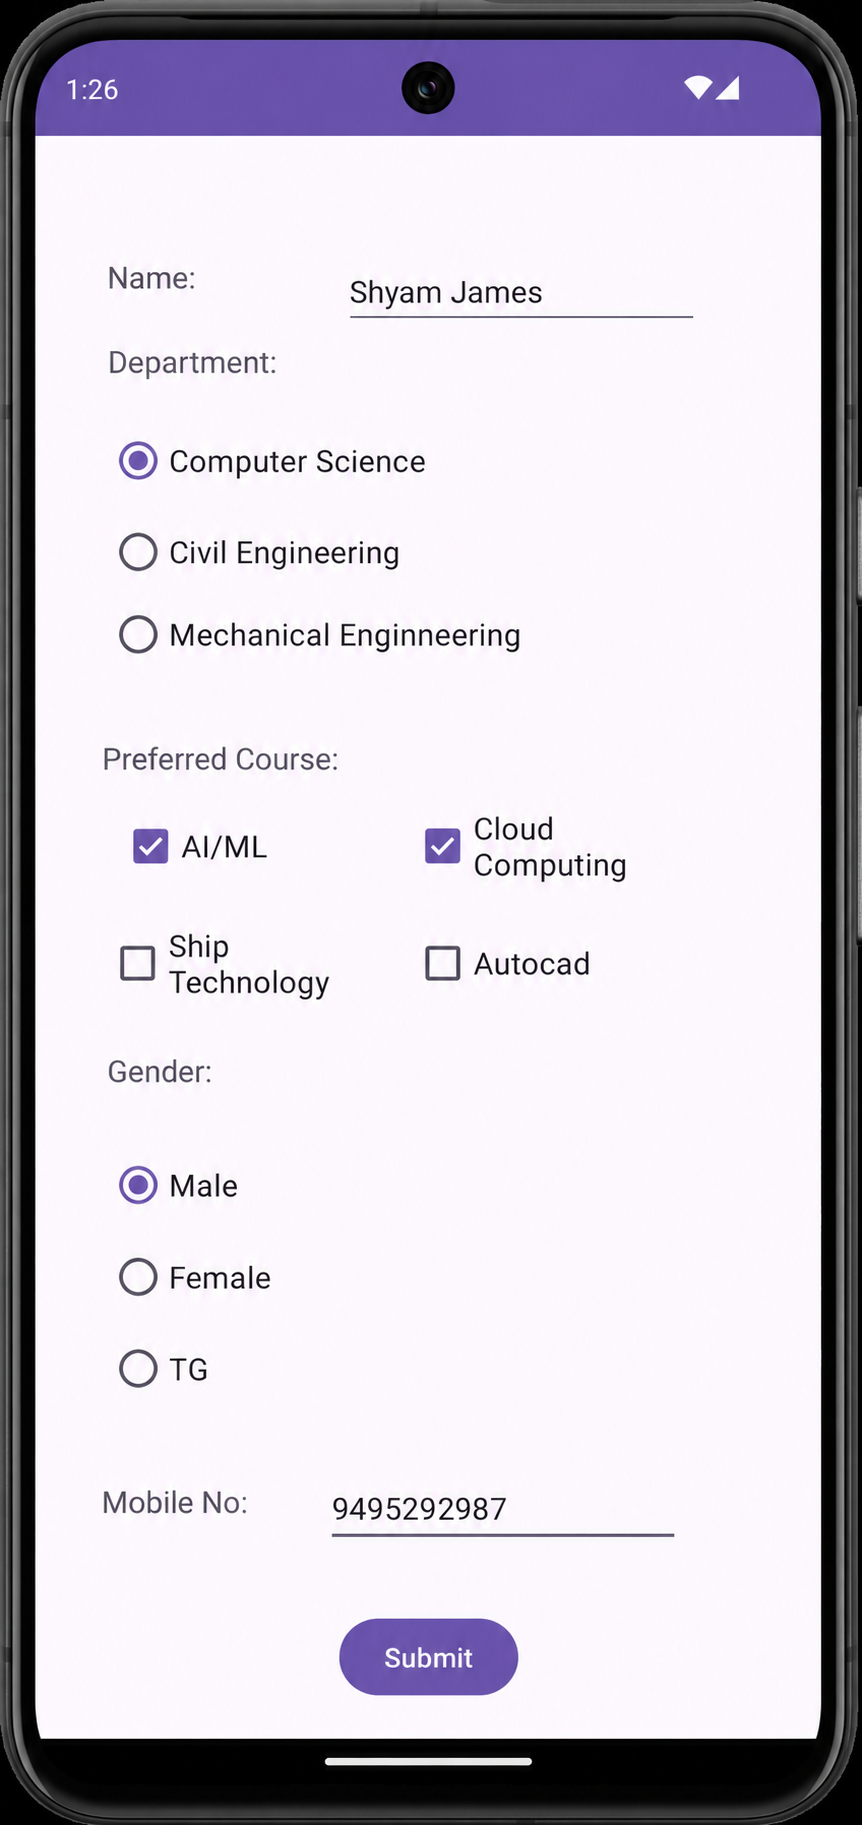
\includegraphics[width=0.4\textwidth]{Output_Screenshots/16_1.png} \quad 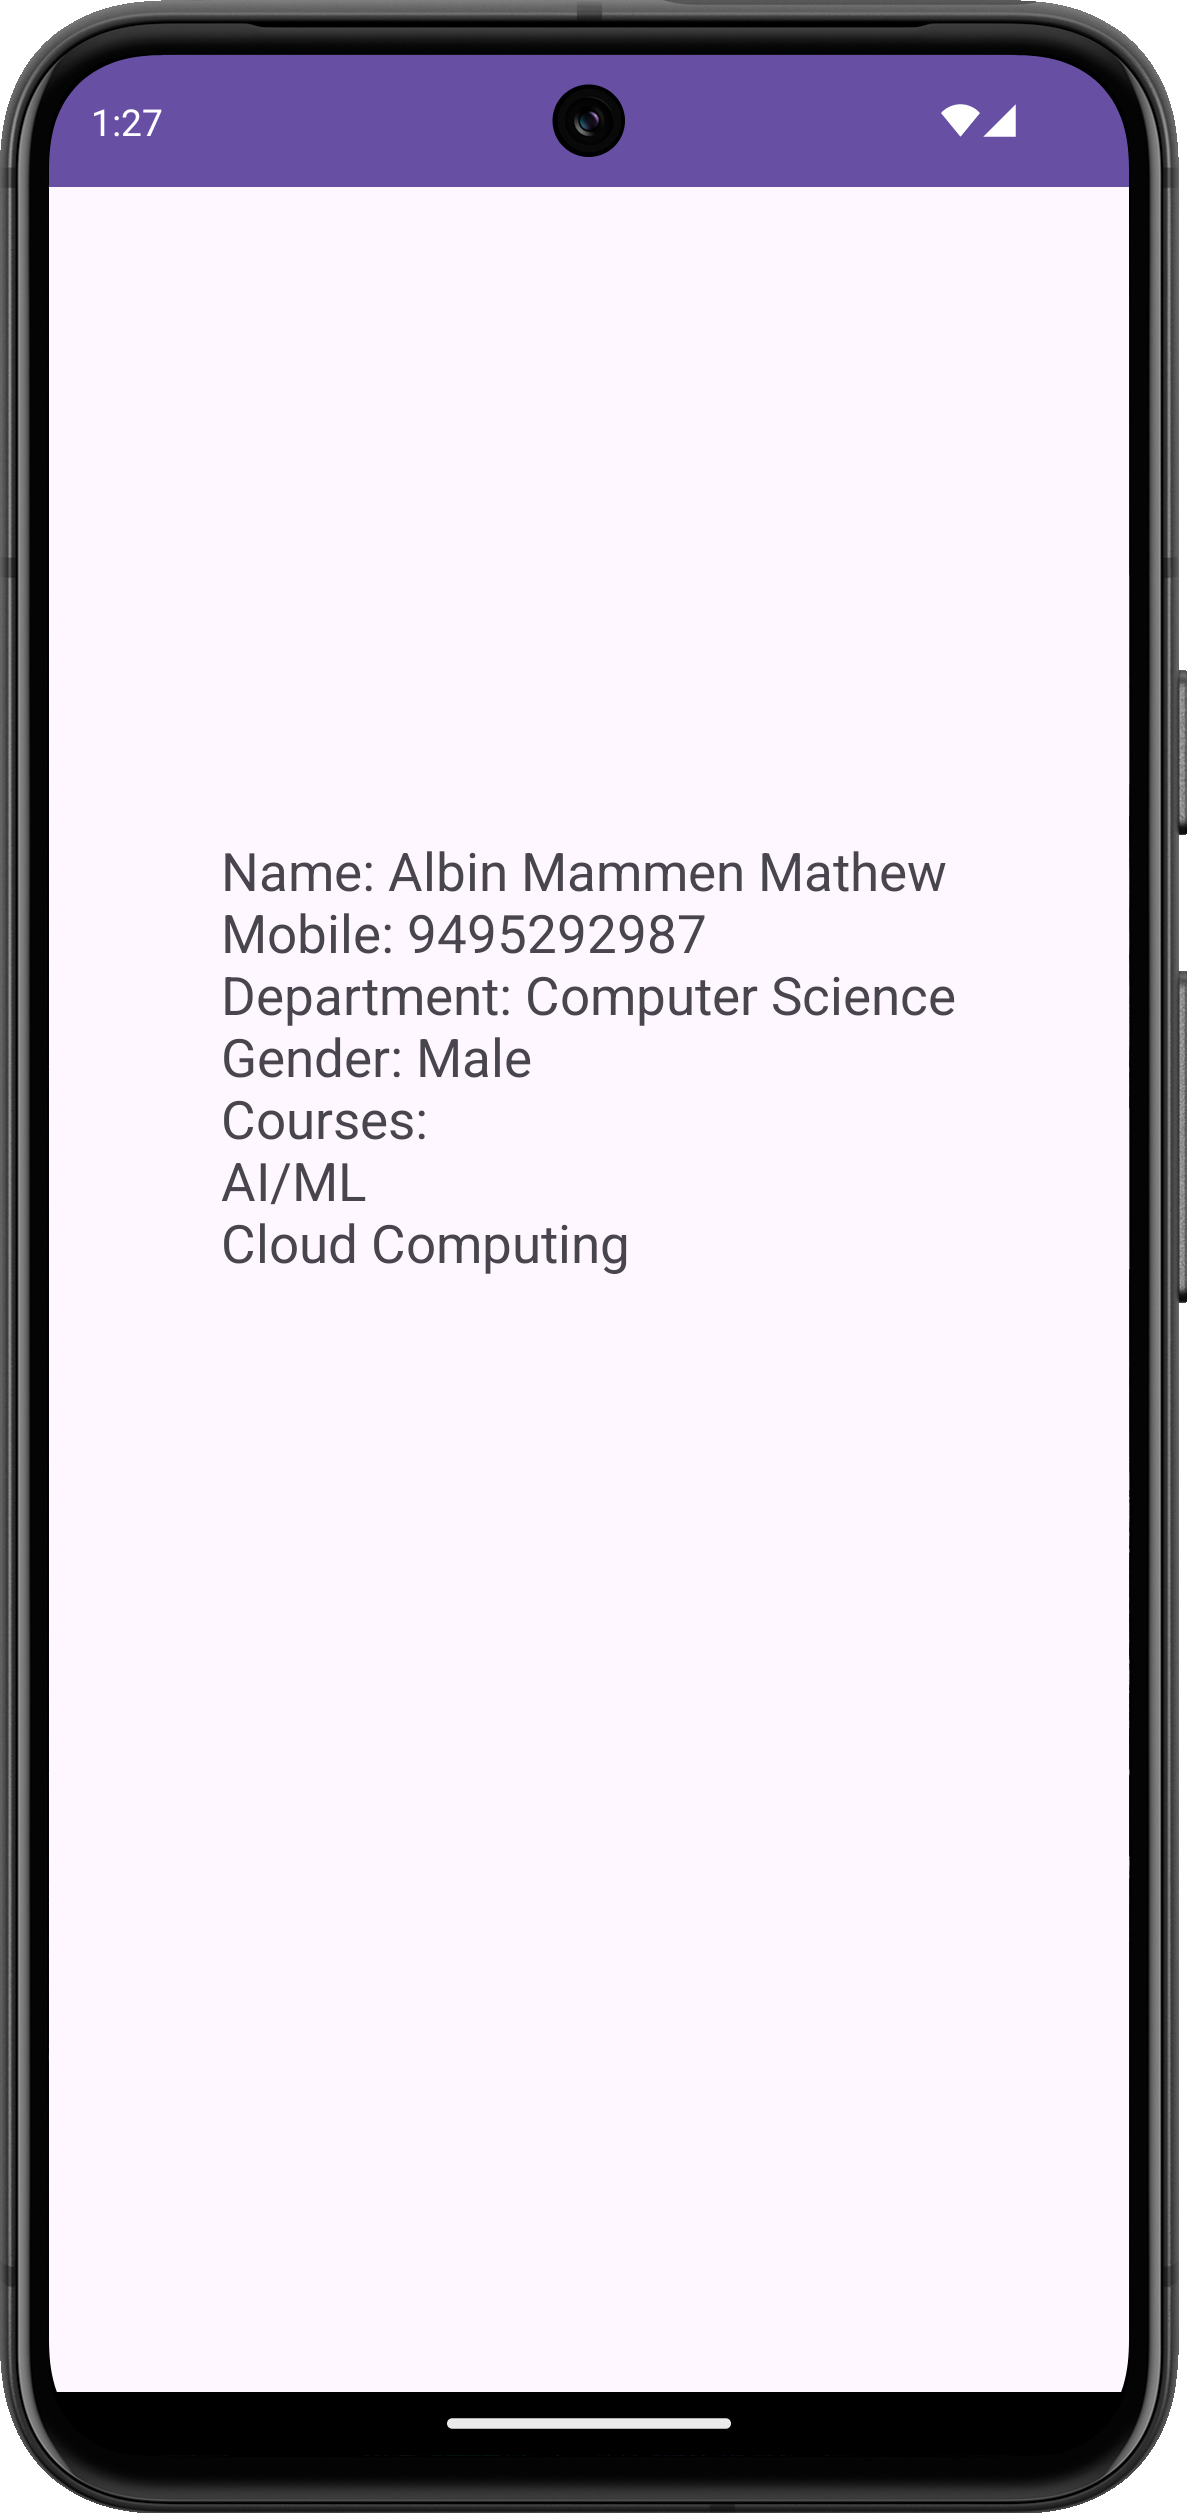
\includegraphics[width=0.4\textwidth]{Output_Screenshots/16_2.png} \end{center} \\
\end{longtable}
\endgroup

\newpage

%% ─── Program 17 ──────────────────────────────────────────────
\noindent\begingroup
\renewcommand{\arraystretch}{1.1}
\begin{longtable}{|p{0.94\textwidth}|}
\hline\endfirsthead\hline\endhead\hline\endfoot\hline\endlastfoot
\rule{0pt}{13pt}Program No: 17 \hfill Date: 29/06/2026 \\
\hline
\rule{0pt}{13pt}Program Title: Create an app that launches a new activity on a button click to calculate and display employee details and salary. \\
\hline
\rule{0pt}{13pt}\textbf{MainActivity.java:} \\
\hline
{\ttfamily\small package\ com.example.pg17\_employeedetails;} \\
\strut \\
{\ttfamily\small import\ android.content.Intent;} \\
{\ttfamily\small import\ android.os.Bundle;} \\
{\ttfamily\small import\ android.view.View;} \\
{\ttfamily\small import\ android.widget.Button;} \\
{\ttfamily\small import\ android.widget.EditText;} \\
{\ttfamily\small import\ androidx.appcompat.app.AppCompatActivity;} \\
\strut \\
{\ttfamily\small public\ class\ MainActivity\ extends\ AppCompatActivity\ \{} \\
{\ttfamily\small \ \ \ \ EditText\ name,\ id,\ sal;} \\
{\ttfamily\small \ \ \ \ Button\ btnNext;} \\
\strut \\
{\ttfamily\small \ \ \ \ @Override} \\
{\ttfamily\small \ \ \ \ protected\ void\ onCreate(Bundle\ savedInstanceState)\ \{} \\
{\ttfamily\small \ \ \ \ \ \ \ \ super.onCreate(savedInstanceState);} \\
{\ttfamily\small \ \ \ \ \ \ \ \ setContentView(R.layout.activity\_main);} \\
\strut \\
{\ttfamily\small \ \ \ \ \ \ \ \ name\ =\ findViewById(R.id.name);} \\
{\ttfamily\small \ \ \ \ \ \ \ \ id\ =\ findViewById(R.id.id);} \\
{\ttfamily\small \ \ \ \ \ \ \ \ sal\ =\ findViewById(R.id.sal);} \\
{\ttfamily\small \ \ \ \ \ \ \ \ btnNext\ =\ findViewById(R.id.btnNext);} \\
\strut \\
{\ttfamily\small \ \ \ \ \ \ \ \ btnNext.setOnClickListener(new\ View.OnClickListener()\ \{} \\
{\ttfamily\small \ \ \ \ \ \ \ \ \ \ \ \ @Override} \\
{\ttfamily\small \ \ \ \ \ \ \ \ \ \ \ \ public\ void\ onClick(View\ view)\ \{} \\
{\ttfamily\small \ \ \ \ \ \ \ \ \ \ \ \ \ \ \ \ Intent\ intent\ =\ new\ Intent(MainActivity.this,\ } \\
{\ttfamily\small \ \ \ \ \ \ \ \ \ \ \ \ \ \ \ \ \ \ \ \ \ \ \ \ \ \ \ \ \ \ \ \ \ \ \ \ \ \ \ \ \ \ \ SecondaryActivity.class);} \\
{\ttfamily\small \ \ \ \ \ \ \ \ \ \ \ \ \ \ \ \ intent.putExtra("name",\ name.getText().toString());} \\
{\ttfamily\small \ \ \ \ \ \ \ \ \ \ \ \ \ \ \ \ intent.putExtra("id",\ id.getText().toString());} \\
{\ttfamily\small \ \ \ \ \ \ \ \ \ \ \ \ \ \ \ \ intent.putExtra("salary",\ sal.getText().toString());} \\
{\ttfamily\small \ \ \ \ \ \ \ \ \ \ \ \ \ \ \ \ startActivity(intent);} \\
{\ttfamily\small \ \ \ \ \ \ \ \ \ \ \ \ \}} \\
{\ttfamily\small \ \ \ \ \ \ \ \ \});} \\
{\ttfamily\small \ \ \ \ \}} \\
{\ttfamily\small \}} \\
\hline
\rule{0pt}{13pt}\textbf{SecondaryActivity.java:} \\
\hline
{\ttfamily\small package\ com.example.pg17\_employeedetails;} \\
\strut \\
{\ttfamily\small import\ android.content.Intent;} \\
{\ttfamily\small import\ android.os.Bundle;} \\
{\ttfamily\small import\ android.widget.TextView;} \\
{\ttfamily\small import\ androidx.appcompat.app.AppCompatActivity;} \\
\strut \\
{\ttfamily\small public\ class\ SecondaryActivity\ extends\ AppCompatActivity\ \{} \\
{\ttfamily\small \ \ \ \ TextView\ result;} \\
\strut \\
{\ttfamily\small \ \ \ \ @Override} \\
{\ttfamily\small \ \ \ \ protected\ void\ onCreate(Bundle\ savedInstanceState)\ \{} \\
{\ttfamily\small \ \ \ \ \ \ \ \ super.onCreate(savedInstanceState);} \\
{\ttfamily\small \ \ \ \ \ \ \ \ setContentView(R.layout.activity\_secondary);} \\
\strut \\
{\ttfamily\small \ \ \ \ \ \ \ \ result\ =\ findViewById(R.id.result);} \\
{\ttfamily\small \ \ \ \ \ \ \ \ Intent\ intent\ =\ getIntent();} \\
\strut \\
{\ttfamily\small \ \ \ \ \ \ \ \ if\ (intent\ !=\ null)\ \{} \\
{\ttfamily\small \ \ \ \ \ \ \ \ \ \ \ \ String\ name\ =\ intent.getStringExtra("name");} \\
{\ttfamily\small \ \ \ \ \ \ \ \ \ \ \ \ String\ id\ =\ intent.getStringExtra("id");} \\
{\ttfamily\small \ \ \ \ \ \ \ \ \ \ \ \ String\ salaryStr\ =\ intent.getStringExtra("salary");} \\
\strut \\
{\ttfamily\small \ \ \ \ \ \ \ \ \ \ \ \ double\ basic\ =\ 0;} \\
{\ttfamily\small \ \ \ \ \ \ \ \ \ \ \ \ try\ \{} \\
{\ttfamily\small \ \ \ \ \ \ \ \ \ \ \ \ \ \ \ \ if\ (salaryStr\ !=\ null)\ \{} \\
{\ttfamily\small \ \ \ \ \ \ \ \ \ \ \ \ \ \ \ \ \ \ \ \ basic\ =\ Double.parseDouble(salaryStr);} \\
{\ttfamily\small \ \ \ \ \ \ \ \ \ \ \ \ \ \ \ \ \}} \\
{\ttfamily\small \ \ \ \ \ \ \ \ \ \ \ \ \}\ catch\ (Exception\ e)\ \{} \\
{\ttfamily\small \ \ \ \ \ \ \ \ \ \ \ \ \ \ \ \ //\ handle\ parsing\ error} \\
{\ttfamily\small \ \ \ \ \ \ \ \ \ \ \ \ \}} \\
\strut \\
{\ttfamily\small \ \ \ \ \ \ \ \ \ \ \ \ double\ hra\ =\ basic\ *\ 0.15;} \\
{\ttfamily\small \ \ \ \ \ \ \ \ \ \ \ \ double\ da\ =\ basic\ *\ 0.10;} \\
{\ttfamily\small \ \ \ \ \ \ \ \ \ \ \ \ double\ gross\ =\ basic\ +\ hra\ +\ da;} \\
\strut \\
{\ttfamily\small \ \ \ \ \ \ \ \ \ \ \ \ result.setText(} \\
{\ttfamily\small \ \ \ \ \ \ \ \ \ \ \ \ \ \ \ \ \ \ \ \ "Employee\ Details\textbackslash{}n\textbackslash{}n"\ +} \\
{\ttfamily\small \ \ \ \ \ \ \ \ \ \ \ \ \ \ \ \ \ \ \ \ "Name\ :\ "\ +\ name\ +} \\
{\ttfamily\small \ \ \ \ \ \ \ \ \ \ \ \ \ \ \ \ \ \ \ \ "\textbackslash{}nEmployee\ ID\ :\ "\ +\ id\ +} \\
{\ttfamily\small \ \ \ \ \ \ \ \ \ \ \ \ \ \ \ \ \ \ \ \ "\textbackslash{}n\textbackslash{}nBasic\ Salary\ :\ "\ +\ basic\ +} \\
{\ttfamily\small \ \ \ \ \ \ \ \ \ \ \ \ \ \ \ \ \ \ \ \ "\textbackslash{}nHRA\ (15\%)\ :\ "\ +\ hra\ +} \\
{\ttfamily\small \ \ \ \ \ \ \ \ \ \ \ \ \ \ \ \ \ \ \ \ "\textbackslash{}nDA\ (10\%)\ :\ "\ +\ da\ +} \\
{\ttfamily\small \ \ \ \ \ \ \ \ \ \ \ \ \ \ \ \ \ \ \ \ "\textbackslash{}nGross\ Salary\ :\ "\ +\ gross} \\
{\ttfamily\small \ \ \ \ \ \ \ \ \ \ \ \ );} \\
{\ttfamily\small \ \ \ \ \ \ \ \ \}} \\
{\ttfamily\small \ \ \ \ \}} \\
{\ttfamily\small \}} \\
\hline
\rule{0pt}{13pt}\textbf{activity\_main.xml:} \\
\hline
{\ttfamily\small \textless{}?xml\ version="1.0"\ encoding="utf-8"?\textgreater{}} \\
{\ttfamily\small \textless{}androidx.constraintlayout.widget.ConstraintLayout\ xmlns:android="http://schemas.android.com/apk/res/android"} \\
{\ttfamily\small \ \ \ \ xmlns:app="http://schemas.android.com/apk/res-auto"} \\
{\ttfamily\small \ \ \ \ android:layout\_width="match\_parent"} \\
{\ttfamily\small \ \ \ \ android:layout\_height="match\_parent"\textgreater{}} \\
\strut \\
{\ttfamily\small \ \ \ \ \textless{}TextView} \\
{\ttfamily\small \ \ \ \ \ \ \ \ android:id="@+id/tvTitle"} \\
{\ttfamily\small \ \ \ \ \ \ \ \ android:layout\_width="wrap\_content"} \\
{\ttfamily\small \ \ \ \ \ \ \ \ android:layout\_height="wrap\_content"} \\
{\ttfamily\small \ \ \ \ \ \ \ \ android:text="Employee\ Details"} \\
{\ttfamily\small \ \ \ \ \ \ \ \ android:textSize="22sp"} \\
{\ttfamily\small \ \ \ \ \ \ \ \ android:textStyle="bold"} \\
{\ttfamily\small \ \ \ \ \ \ \ \ app:layout\_constraintBottom\_toBottomOf="parent"} \\
{\ttfamily\small \ \ \ \ \ \ \ \ app:layout\_constraintEnd\_toEndOf="parent"} \\
{\ttfamily\small \ \ \ \ \ \ \ \ app:layout\_constraintHorizontal\_bias="0.587"} \\
{\ttfamily\small \ \ \ \ \ \ \ \ app:layout\_constraintStart\_toStartOf="parent"} \\
{\ttfamily\small \ \ \ \ \ \ \ \ app:layout\_constraintTop\_toTopOf="parent"} \\
{\ttfamily\small \ \ \ \ \ \ \ \ app:layout\_constraintVertical\_bias="0.067"\ /\textgreater{}} \\
\strut \\
{\ttfamily\small \ \ \ \ \textless{}TextView} \\
{\ttfamily\small \ \ \ \ \ \ \ \ android:id="@+id/tvName"} \\
{\ttfamily\small \ \ \ \ \ \ \ \ android:layout\_width="wrap\_content"} \\
{\ttfamily\small \ \ \ \ \ \ \ \ android:layout\_height="wrap\_content"} \\
{\ttfamily\small \ \ \ \ \ \ \ \ android:layout\_marginStart="20dp"} \\
{\ttfamily\small \ \ \ \ \ \ \ \ android:layout\_marginTop="20dp"} \\
{\ttfamily\small \ \ \ \ \ \ \ \ android:text="Employee\ Name"} \\
{\ttfamily\small \ \ \ \ \ \ \ \ app:layout\_constraintStart\_toStartOf="parent"} \\
{\ttfamily\small \ \ \ \ \ \ \ \ app:layout\_constraintTop\_toBottomOf="@id/tvTitle"\ /\textgreater{}} \\
\strut \\
{\ttfamily\small \ \ \ \ \textless{}EditText} \\
{\ttfamily\small \ \ \ \ \ \ \ \ android:id="@+id/name"} \\
{\ttfamily\small \ \ \ \ \ \ \ \ android:layout\_width="250dp"} \\
{\ttfamily\small \ \ \ \ \ \ \ \ android:layout\_height="wrap\_content"} \\
{\ttfamily\small \ \ \ \ \ \ \ \ android:hint="Enter\ Name"} \\
{\ttfamily\small \ \ \ \ \ \ \ \ app:layout\_constraintStart\_toStartOf="@id/tvName"} \\
{\ttfamily\small \ \ \ \ \ \ \ \ app:layout\_constraintTop\_toBottomOf="@id/tvName"\ /\textgreater{}} \\
\strut \\
{\ttfamily\small \ \ \ \ \textless{}TextView} \\
{\ttfamily\small \ \ \ \ \ \ \ \ android:id="@+id/tvId"} \\
{\ttfamily\small \ \ \ \ \ \ \ \ android:layout\_width="wrap\_content"} \\
{\ttfamily\small \ \ \ \ \ \ \ \ android:layout\_height="wrap\_content"} \\
{\ttfamily\small \ \ \ \ \ \ \ \ android:layout\_marginTop="15dp"} \\
{\ttfamily\small \ \ \ \ \ \ \ \ android:text="Employee\ ID"} \\
{\ttfamily\small \ \ \ \ \ \ \ \ app:layout\_constraintStart\_toStartOf="@id/tvName"} \\
{\ttfamily\small \ \ \ \ \ \ \ \ app:layout\_constraintTop\_toBottomOf="@id/name"\ /\textgreater{}} \\
\strut \\
{\ttfamily\small \ \ \ \ \textless{}EditText} \\
{\ttfamily\small \ \ \ \ \ \ \ \ android:id="@+id/id"} \\
{\ttfamily\small \ \ \ \ \ \ \ \ android:layout\_width="250dp"} \\
{\ttfamily\small \ \ \ \ \ \ \ \ android:layout\_height="wrap\_content"} \\
{\ttfamily\small \ \ \ \ \ \ \ \ android:hint="Enter\ ID"} \\
{\ttfamily\small \ \ \ \ \ \ \ \ app:layout\_constraintStart\_toStartOf="@id/tvName"} \\
{\ttfamily\small \ \ \ \ \ \ \ \ app:layout\_constraintTop\_toBottomOf="@id/tvId"\ /\textgreater{}} \\
\strut \\
{\ttfamily\small \ \ \ \ \textless{}TextView} \\
{\ttfamily\small \ \ \ \ \ \ \ \ android:id="@+id/tvSalary"} \\
{\ttfamily\small \ \ \ \ \ \ \ \ android:layout\_width="wrap\_content"} \\
{\ttfamily\small \ \ \ \ \ \ \ \ android:layout\_height="wrap\_content"} \\
{\ttfamily\small \ \ \ \ \ \ \ \ android:layout\_marginTop="15dp"} \\
{\ttfamily\small \ \ \ \ \ \ \ \ android:text="Basic\ Salary"} \\
{\ttfamily\small \ \ \ \ \ \ \ \ app:layout\_constraintStart\_toStartOf="@id/tvName"} \\
{\ttfamily\small \ \ \ \ \ \ \ \ app:layout\_constraintTop\_toBottomOf="@id/id"\ /\textgreater{}} \\
\strut \\
{\ttfamily\small \ \ \ \ \textless{}EditText} \\
{\ttfamily\small \ \ \ \ \ \ \ \ android:id="@+id/sal"} \\
{\ttfamily\small \ \ \ \ \ \ \ \ android:layout\_width="250dp"} \\
{\ttfamily\small \ \ \ \ \ \ \ \ android:layout\_height="wrap\_content"} \\
{\ttfamily\small \ \ \ \ \ \ \ \ android:hint="Enter\ Salary"} \\
{\ttfamily\small \ \ \ \ \ \ \ \ android:inputType="numberDecimal"} \\
{\ttfamily\small \ \ \ \ \ \ \ \ app:layout\_constraintStart\_toStartOf="@id/tvName"} \\
{\ttfamily\small \ \ \ \ \ \ \ \ app:layout\_constraintTop\_toBottomOf="@id/tvSalary"\ /\textgreater{}} \\
\strut \\
{\ttfamily\small \ \ \ \ \textless{}Button} \\
{\ttfamily\small \ \ \ \ \ \ \ \ android:id="@+id/btnNext"} \\
{\ttfamily\small \ \ \ \ \ \ \ \ android:layout\_width="wrap\_content"} \\
{\ttfamily\small \ \ \ \ \ \ \ \ android:layout\_height="wrap\_content"} \\
{\ttfamily\small \ \ \ \ \ \ \ \ android:layout\_marginTop="25dp"} \\
{\ttfamily\small \ \ \ \ \ \ \ \ android:text="Show\ Details"} \\
{\ttfamily\small \ \ \ \ \ \ \ \ app:layout\_constraintEnd\_toEndOf="parent"} \\
{\ttfamily\small \ \ \ \ \ \ \ \ app:layout\_constraintStart\_toStartOf="parent"} \\
{\ttfamily\small \ \ \ \ \ \ \ \ app:layout\_constraintTop\_toBottomOf="@id/sal"\ /\textgreater{}} \\
\strut \\
{\ttfamily\small \textless{}/androidx.constraintlayout.widget.ConstraintLayout\textgreater{}} \\
\hline
\rule{0pt}{13pt}\textbf{activity\_secondary.xml:} \\
\hline
{\ttfamily\small \textless{}?xml\ version="1.0"\ encoding="utf-8"?\textgreater{}} \\
{\ttfamily\small \textless{}androidx.constraintlayout.widget.ConstraintLayout\ xmlns:android="http://schemas.android.com/apk/res/android"} \\
{\ttfamily\small \ \ \ \ xmlns:app="http://schemas.android.com/apk/res-auto"} \\
{\ttfamily\small \ \ \ \ android:layout\_width="match\_parent"} \\
{\ttfamily\small \ \ \ \ android:layout\_height="match\_parent"\textgreater{}} \\
\strut \\
{\ttfamily\small \ \ \ \ \textless{}TextView} \\
{\ttfamily\small \ \ \ \ \ \ \ \ android:id="@+id/result"} \\
{\ttfamily\small \ \ \ \ \ \ \ \ android:layout\_width="300dp"} \\
{\ttfamily\small \ \ \ \ \ \ \ \ android:layout\_height="wrap\_content"} \\
{\ttfamily\small \ \ \ \ \ \ \ \ android:gravity="center"} \\
{\ttfamily\small \ \ \ \ \ \ \ \ android:textSize="18sp"} \\
{\ttfamily\small \ \ \ \ \ \ \ \ android:textStyle="bold"} \\
{\ttfamily\small \ \ \ \ \ \ \ \ app:layout\_constraintBottom\_toBottomOf="parent"} \\
{\ttfamily\small \ \ \ \ \ \ \ \ app:layout\_constraintEnd\_toEndOf="parent"} \\
{\ttfamily\small \ \ \ \ \ \ \ \ app:layout\_constraintStart\_toStartOf="parent"} \\
{\ttfamily\small \ \ \ \ \ \ \ \ app:layout\_constraintTop\_toTopOf="parent"\ /\textgreater{}} \\
\strut \\
{\ttfamily\small \textless{}/androidx.constraintlayout.widget.ConstraintLayout\textgreater{}} \\
\hline
Output: \newline \begin{center} 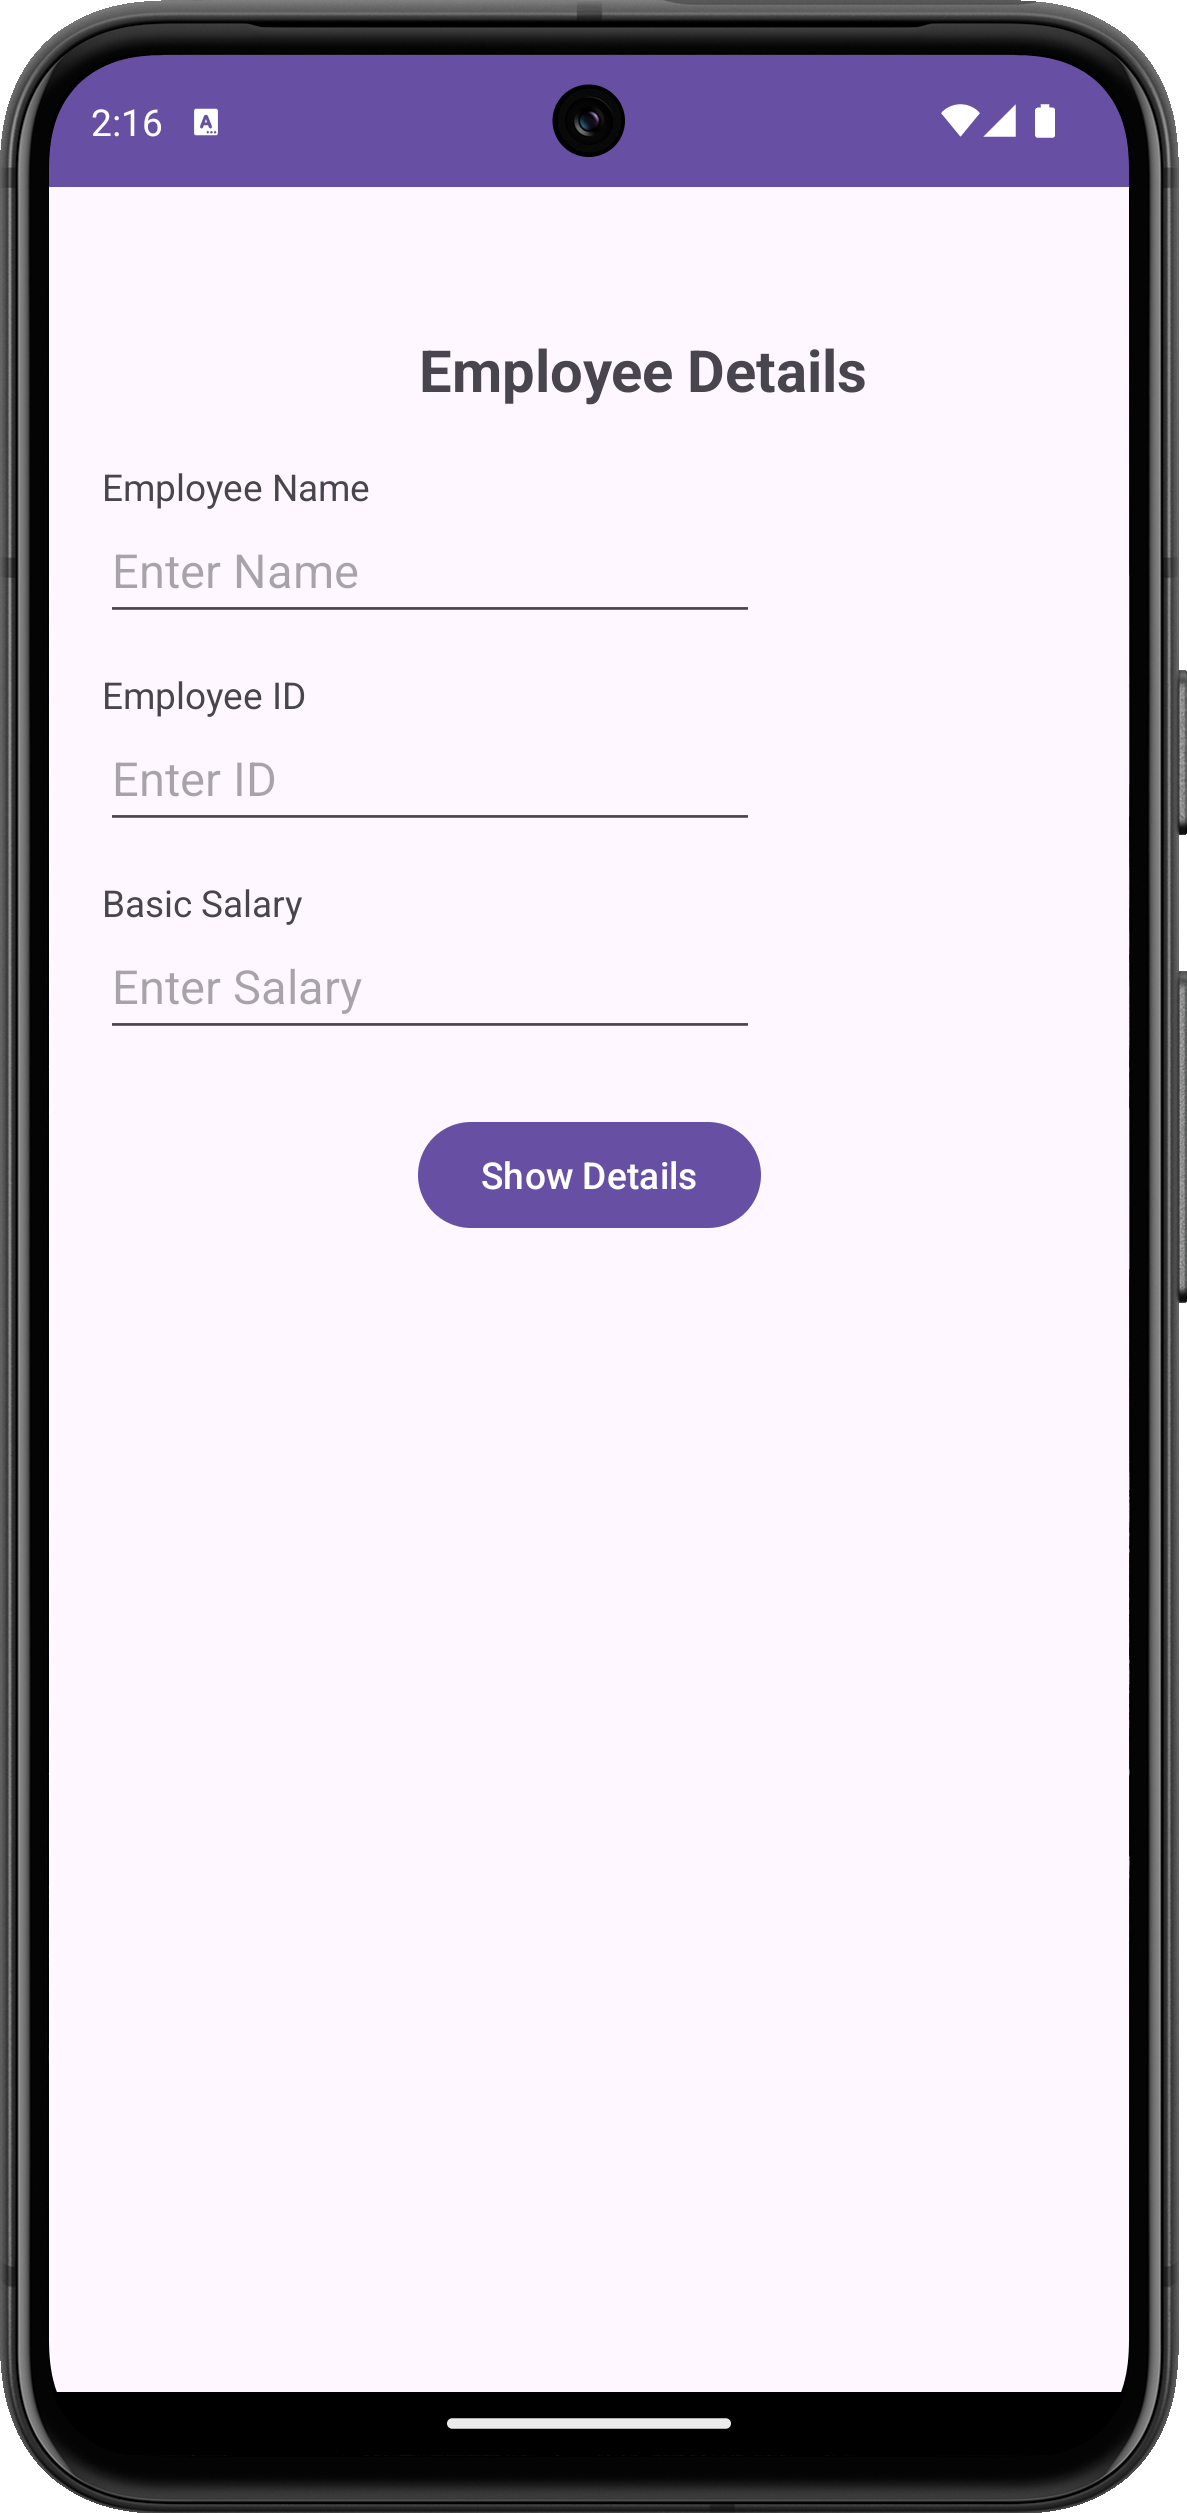
\includegraphics[width=0.4\textwidth]{Output_Screenshots/17_1.png} \quad 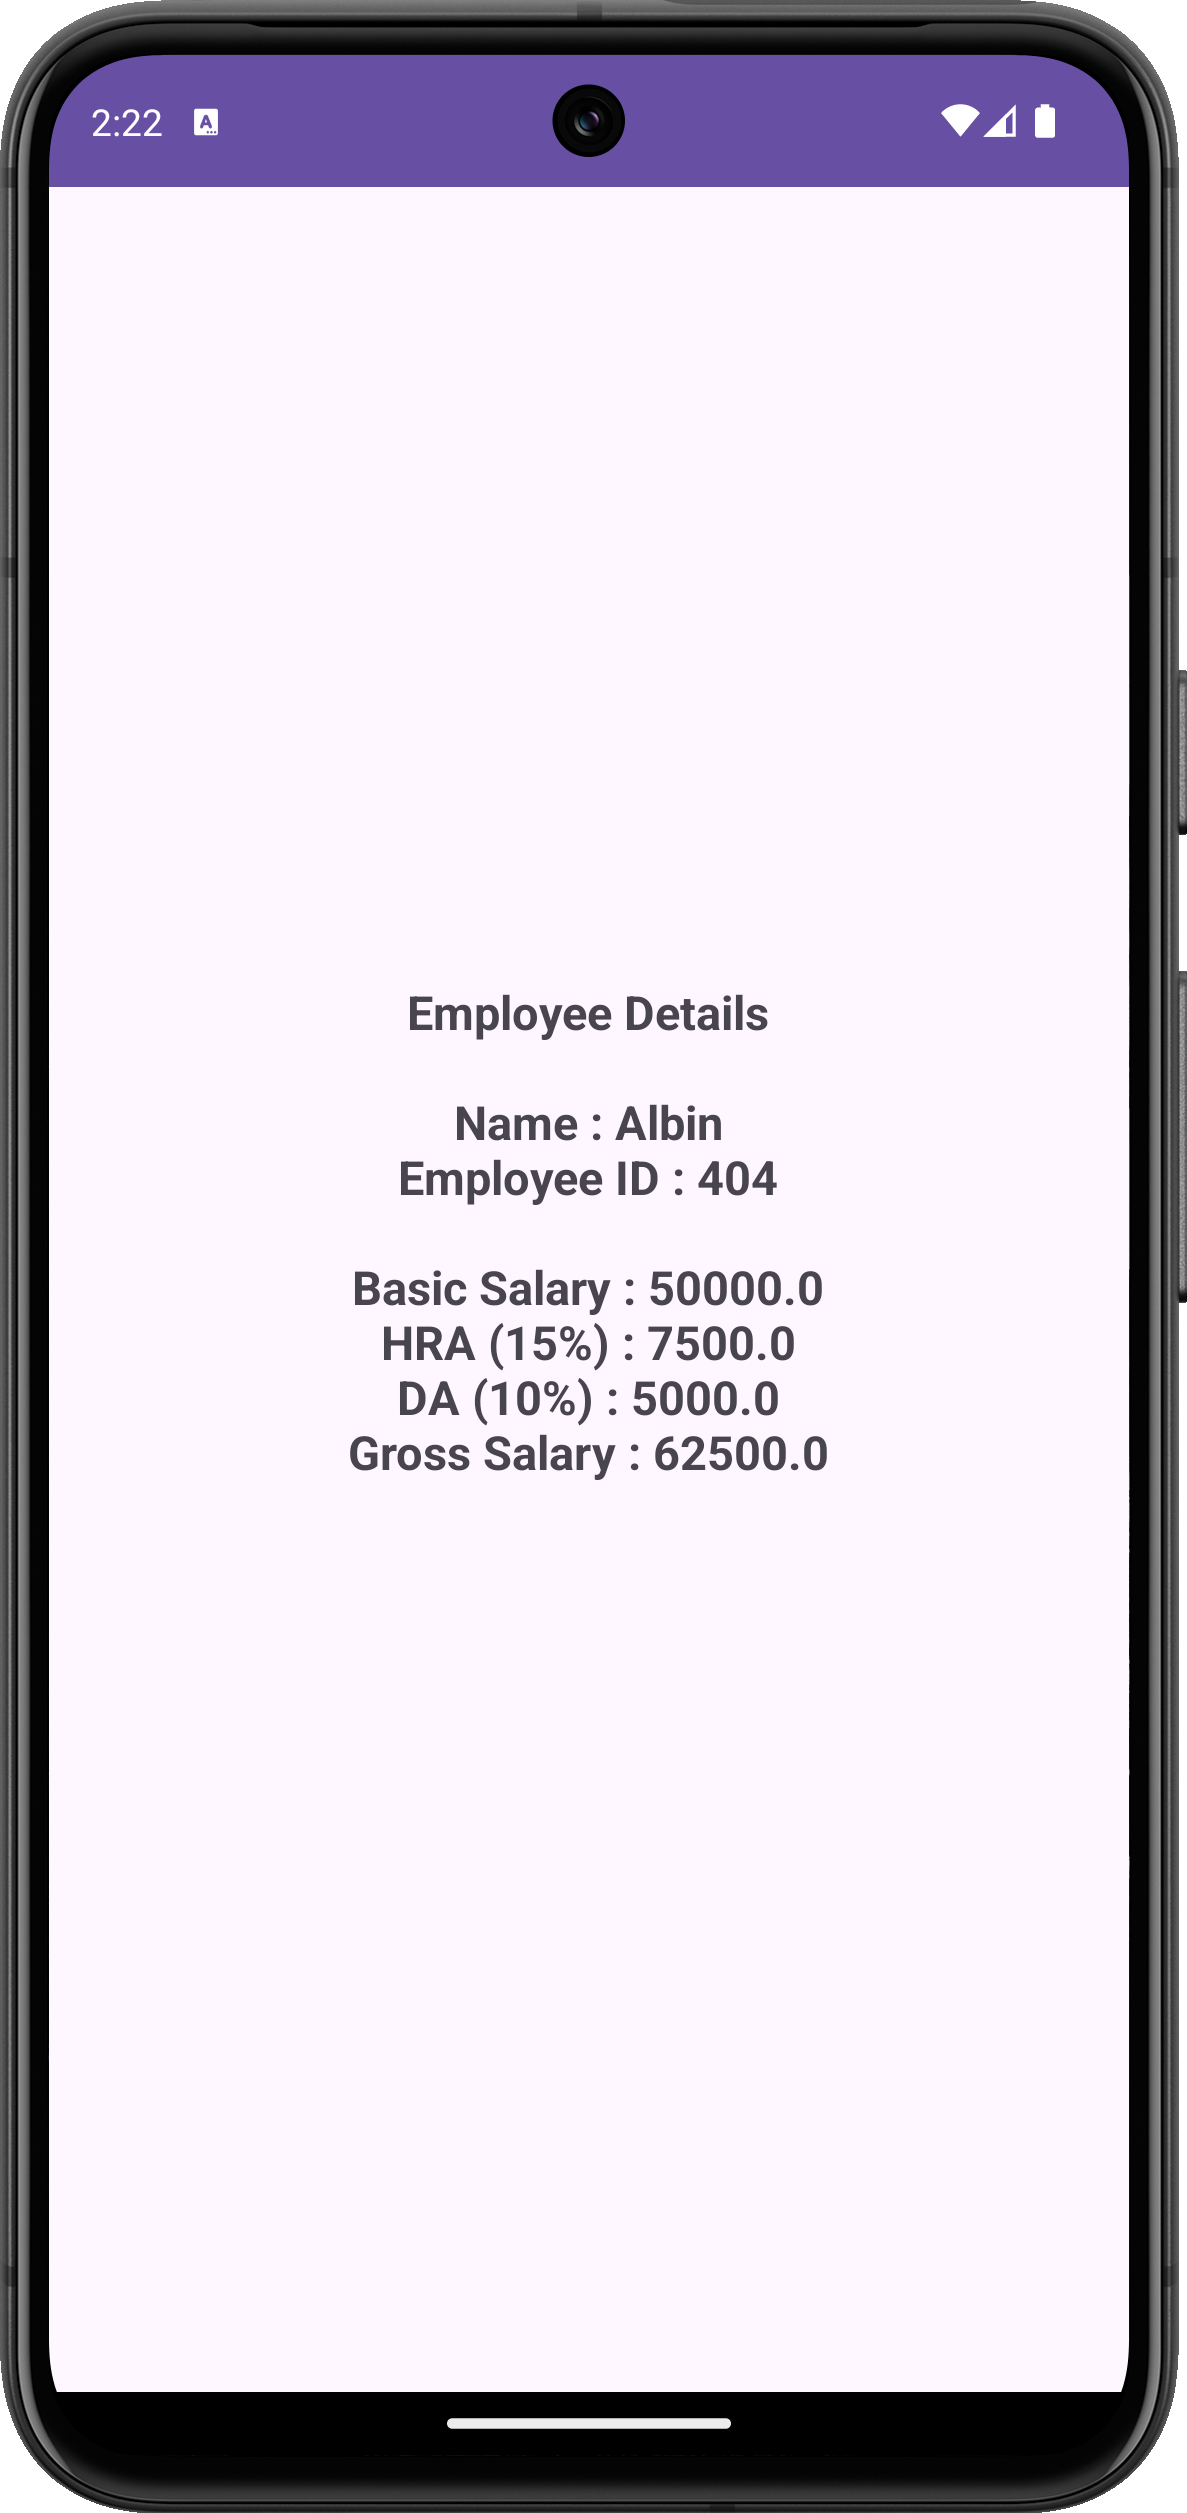
\includegraphics[width=0.4\textwidth]{Output_Screenshots/17_2.png} \end{center} \\
\end{longtable}
\endgroup

\newpage

%% ─── Program 18 ──────────────────────────────────────────────
\noindent\begingroup
\renewcommand{\arraystretch}{1.1}
\begin{longtable}{|p{0.94\textwidth}|}
\hline\endfirsthead\hline\endhead\hline\endfoot\hline\endlastfoot
\rule{0pt}{13pt}Program No: 18 \hfill Date: 29/06/2026 \\
\hline
\rule{0pt}{13pt}Program Title: Create an app to broadcast a custom intent. \\
\hline
\rule{0pt}{13pt}\textbf{MainActivity.java:} \\
\hline
{\ttfamily\small package\ com.example.broadcast;} \\
\strut \\
{\ttfamily\small import\ android.content.Intent;} \\
{\ttfamily\small import\ android.os.Bundle;} \\
{\ttfamily\small import\ androidx.appcompat.app.AppCompatActivity;} \\
{\ttfamily\small import\ android.widget.Button;} \\
\strut \\
{\ttfamily\small public\ class\ MainActivity\ extends\ AppCompatActivity\ \{} \\
\strut \\
{\ttfamily\small \ \ \ \ public\ static\ final\ String\ MY\_ACTION\ =\ } \\
{\ttfamily\small \ \ \ \ \ \ \ \ \ \ \ \ "com.example.broadcast.MY\_ACTION";} \\
\strut \\
{\ttfamily\small \ \ \ \ @Override} \\
{\ttfamily\small \ \ \ \ protected\ void\ onCreate(Bundle\ savedInstanceState)\ \{} \\
{\ttfamily\small \ \ \ \ \ \ \ \ super.onCreate(savedInstanceState);} \\
{\ttfamily\small \ \ \ \ \ \ \ \ setContentView(R.layout.activity\_main);} \\
{\ttfamily\small \ \ \ \ \ \ \ \ Button\ send\ =\ findViewById(R.id.send);} \\
{\ttfamily\small \ \ \ \ \ \ \ \ send.setOnClickListener(v\ -\textgreater{}\ \{} \\
{\ttfamily\small \ \ \ \ \ \ \ \ \ \ \ \ Intent\ intent\ =\ new\ Intent(MY\_ACTION);} \\
{\ttfamily\small \ \ \ \ \ \ \ \ \ \ \ \ intent.putExtra("message",\ "Hello\ from\ MainActivity!!");} \\
{\ttfamily\small \ \ \ \ \ \ \ \ \ \ \ \ intent.setPackage(getPackageName());} \\
{\ttfamily\small \ \ \ \ \ \ \ \ \ \ \ \ sendBroadcast(intent);} \\
{\ttfamily\small \ \ \ \ \ \ \ \ \});} \\
{\ttfamily\small \ \ \ \ \}} \\
{\ttfamily\small \}} \\
\hline
\rule{0pt}{13pt}\textbf{MyReceiver.java:} \\
\hline
{\ttfamily\small package\ com.example.broadcast;} \\
\strut \\
{\ttfamily\small import\ android.content.BroadcastReceiver;} \\
{\ttfamily\small import\ android.content.Context;} \\
{\ttfamily\small import\ android.content.Intent;} \\
{\ttfamily\small import\ android.widget.Toast;} \\
\strut \\
{\ttfamily\small public\ class\ MyReceiver\ extends\ BroadcastReceiver\ \{} \\
\strut \\
{\ttfamily\small \ \ \ \ @Override} \\
{\ttfamily\small \ \ \ \ public\ void\ onReceive(Context\ context,\ Intent\ intent)\ \{} \\
{\ttfamily\small \ \ \ \ \ \ \ \ String\ message\ =\ intent.getStringExtra("message");} \\
{\ttfamily\small \ \ \ \ \ \ \ \ Toast.makeText(context,\ "Custom\ Broadcast\ Received:\ "\ +\ message,} \\
{\ttfamily\small \ \ \ \ \ \ \ \ \ \ \ \ \ \ \ \ Toast.LENGTH\_SHORT).show();} \\
{\ttfamily\small \ \ \ \ \}} \\
{\ttfamily\small \}} \\
\hline
\rule{0pt}{13pt}\textbf{activity\_main.xml:} \\
\hline
{\ttfamily\small \textless{}?xml\ version="1.0"\ encoding="utf-8"?\textgreater{}} \\
{\ttfamily\small \textless{}androidx.constraintlayout.widget.ConstraintLayout} \\
{\ttfamily\small \ \ \ \ xmlns:android="http://schemas.android.com/apk/res/android"} \\
{\ttfamily\small \ \ \ \ xmlns:app="http://schemas.android.com/apk/res-auto"} \\
{\ttfamily\small \ \ \ \ xmlns:tools="http://schemas.android.com/tools"} \\
{\ttfamily\small \ \ \ \ android:id="@+id/main"} \\
{\ttfamily\small \ \ \ \ android:layout\_width="match\_parent"} \\
{\ttfamily\small \ \ \ \ android:layout\_height="match\_parent"} \\
{\ttfamily\small \ \ \ \ tools:context=".MainActivity"\textgreater{}} \\
\strut \\
{\ttfamily\small \ \ \ \ \textless{}Button} \\
{\ttfamily\small \ \ \ \ \ \ \ \ android:id="@+id/send"} \\
{\ttfamily\small \ \ \ \ \ \ \ \ android:layout\_width="wrap\_content"} \\
{\ttfamily\small \ \ \ \ \ \ \ \ android:layout\_height="wrap\_content"} \\
{\ttfamily\small \ \ \ \ \ \ \ \ android:text="Send"} \\
{\ttfamily\small \ \ \ \ \ \ \ \ app:layout\_constraintBottom\_toBottomOf="parent"} \\
{\ttfamily\small \ \ \ \ \ \ \ \ app:layout\_constraintEnd\_toEndOf="parent"} \\
{\ttfamily\small \ \ \ \ \ \ \ \ app:layout\_constraintHorizontal\_bias="0.52"} \\
{\ttfamily\small \ \ \ \ \ \ \ \ app:layout\_constraintStart\_toStartOf="parent"} \\
{\ttfamily\small \ \ \ \ \ \ \ \ app:layout\_constraintTop\_toTopOf="parent"} \\
{\ttfamily\small \ \ \ \ \ \ \ \ app:layout\_constraintVertical\_bias="0.614"\ /\textgreater{}} \\
\strut \\
{\ttfamily\small \textless{}/androidx.constraintlayout.widget.ConstraintLayout\textgreater{}} \\
\hline
\rule{0pt}{13pt}\textbf{AndroidManifest.xml:} \\
\hline
{\ttfamily\small \textless{}receiver} \\
{\ttfamily\small \ \ \ \ android:name=".MyReceiver"} \\
{\ttfamily\small \ \ \ \ android:enabled="true"} \\
{\ttfamily\small \ \ \ \ android:exported="true"\textgreater{}} \\
{\ttfamily\small \ \ \ \ \textless{}intent-filter\textgreater{}} \\
{\ttfamily\small \ \ \ \ \ \ \ \ \textless{}action\ android:name="com.example.broadcast.MY\_ACTION"\ /\textgreater{}} \\
{\ttfamily\small \ \ \ \ \textless{}/intent-filter\textgreater{}} \\
{\ttfamily\small \textless{}/receiver\textgreater{}} \\
\hline
Output: \newline \begin{center} 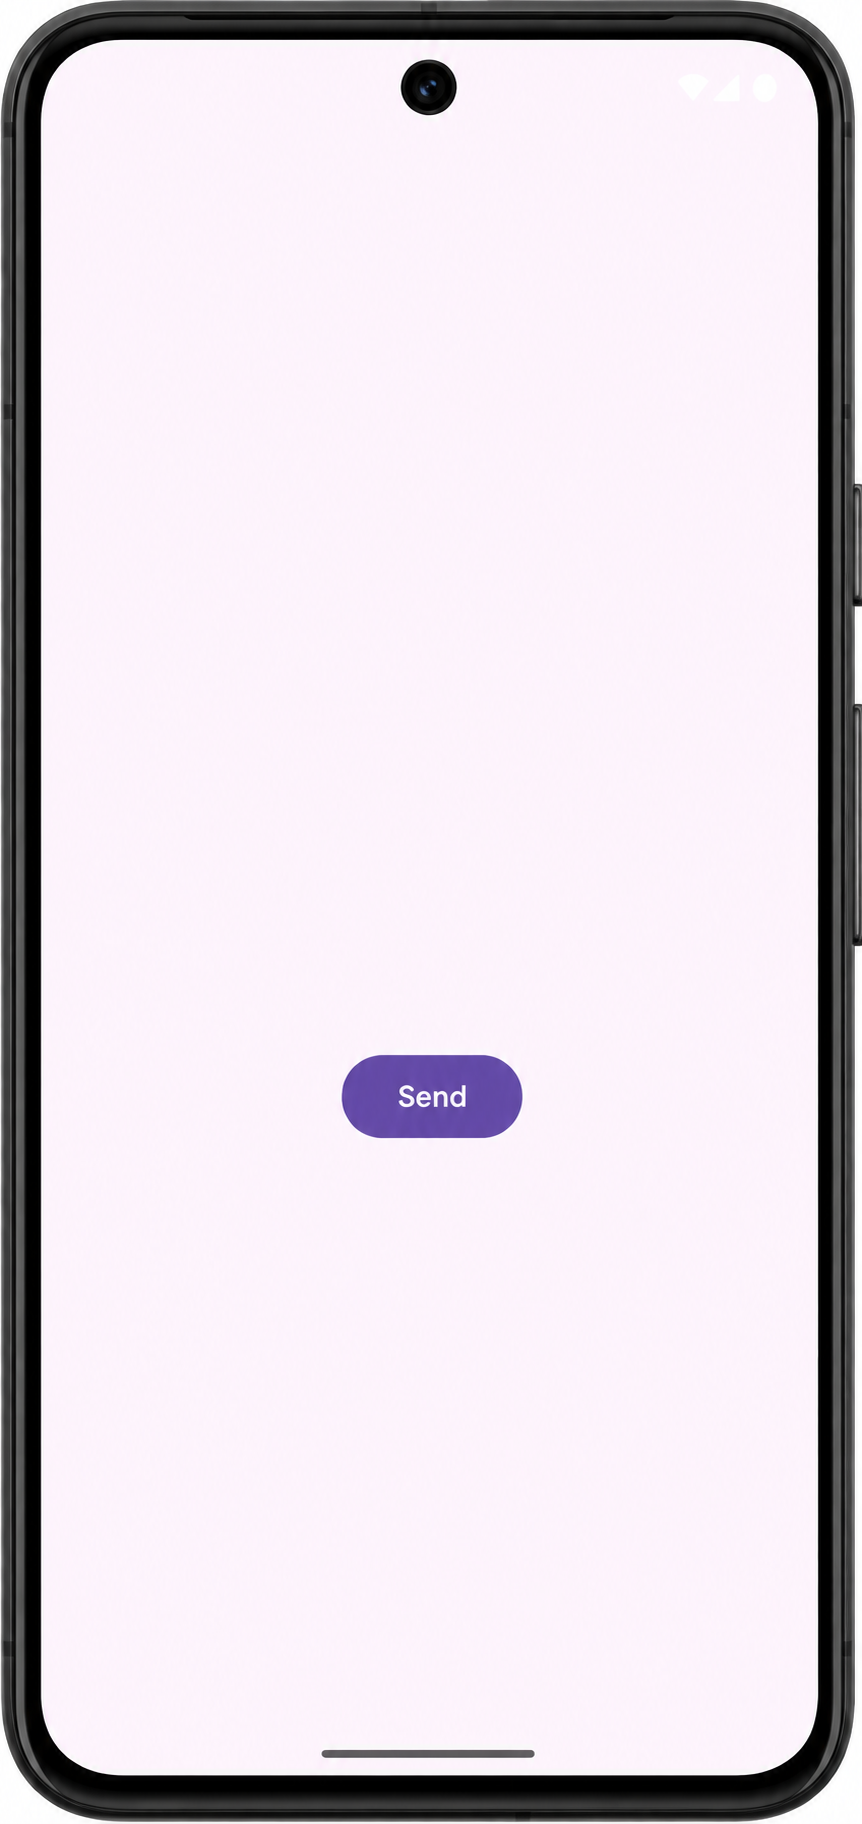
\includegraphics[width=0.4\textwidth]{Output_Screenshots/18_1.png} \quad 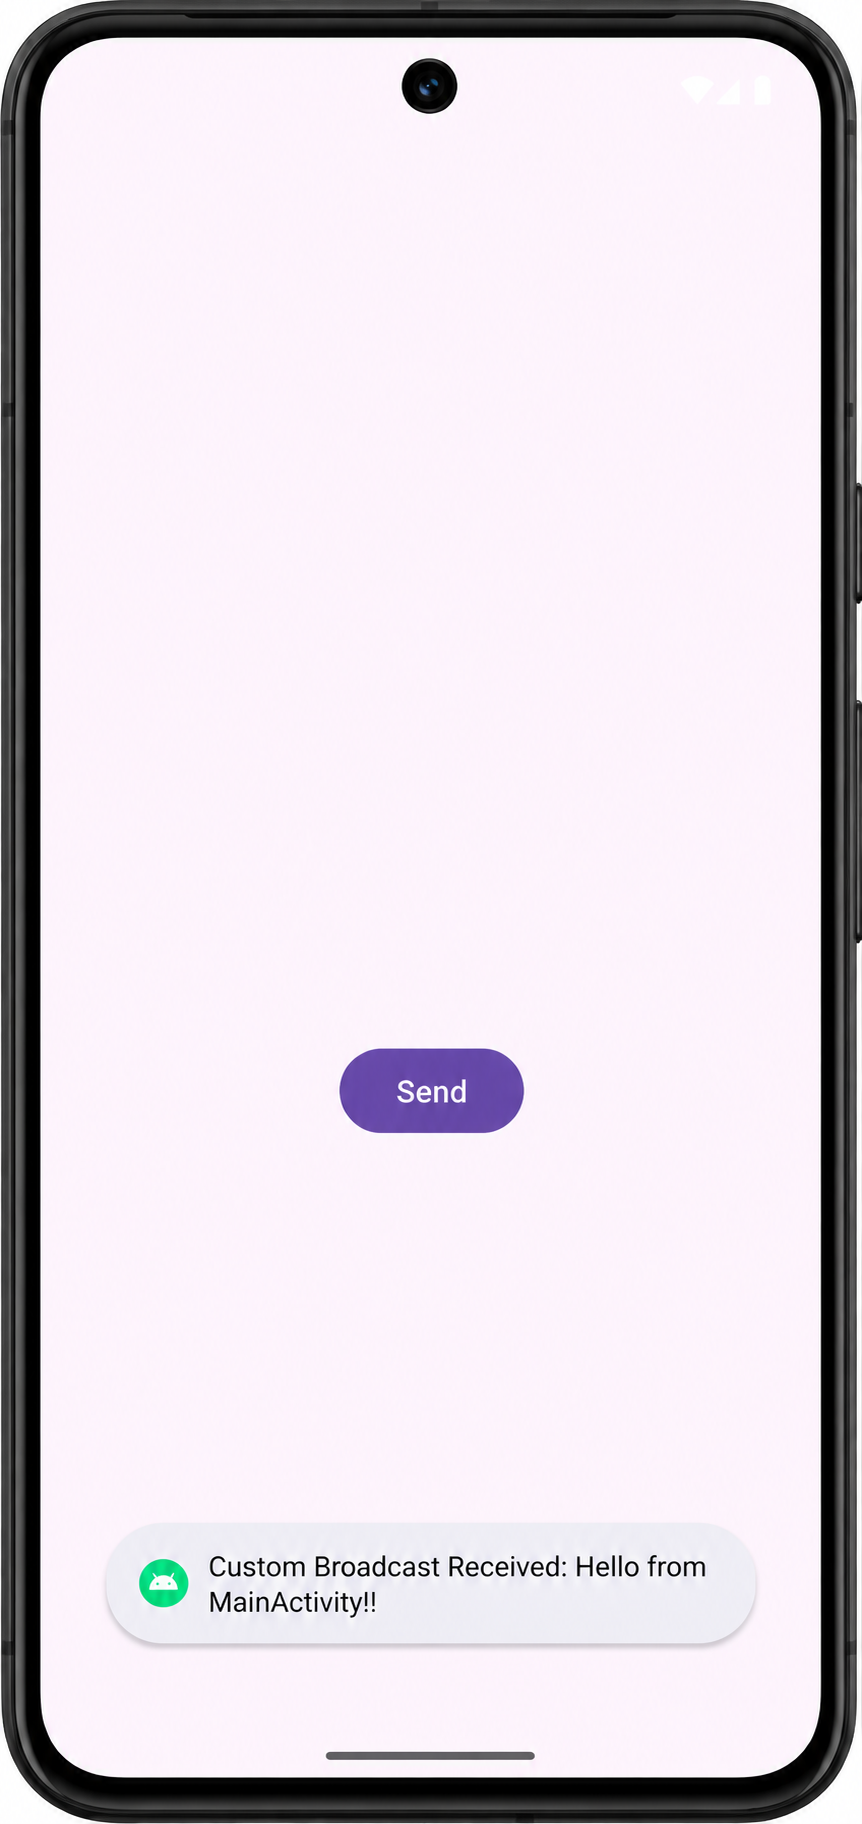
\includegraphics[width=0.4\textwidth]{Output_Screenshots/18_2.png} \end{center} \\
\end{longtable}
\endgroup

\newpage

%% ─── Program 19 ──────────────────────────────────────────────
\noindent\begingroup
\renewcommand{\arraystretch}{1.1}
\begin{longtable}{|p{0.94\textwidth}|}
\hline\endfirsthead\hline\endhead\hline\endfoot\hline\endlastfoot
\rule{0pt}{13pt}Program No: 19 \hfill Date: 29/06/2026 \\
\hline
\rule{0pt}{13pt}Program Title: Create an app to broadcast a system intent (AIRPLANE MODE CHANGED). \\
\hline
\rule{0pt}{13pt}\textbf{MainActivity.java:} \\
\hline
{\ttfamily\small package\ com.example.pg19\_airplanemode;} \\
\strut \\
{\ttfamily\small import\ android.content.Intent;} \\
{\ttfamily\small import\ android.content.IntentFilter;} \\
{\ttfamily\small import\ android.os.Bundle;} \\
{\ttfamily\small import\ androidx.appcompat.app.AppCompatActivity;} \\
\strut \\
{\ttfamily\small public\ class\ MainActivity\ extends\ AppCompatActivity\ \{} \\
{\ttfamily\small \ \ \ \ private\ final\ AirplaneModeReceiver\ receiver\ =\ new\ AirplaneModeReceiver();} \\
\strut \\
{\ttfamily\small \ \ \ \ @Override} \\
{\ttfamily\small \ \ \ \ protected\ void\ onCreate(Bundle\ savedInstanceState)\ \{} \\
{\ttfamily\small \ \ \ \ \ \ \ \ super.onCreate(savedInstanceState);} \\
{\ttfamily\small \ \ \ \ \ \ \ \ setContentView(R.layout.activity\_main);} \\
{\ttfamily\small \ \ \ \ \ \ \ \ IntentFilter\ filter\ =\ } \\
{\ttfamily\small \ \ \ \ \ \ \ \ \ \ \ \ \ \ \ \ new\ IntentFilter(Intent.ACTION\_AIRPLANE\_MODE\_CHANGED);} \\
{\ttfamily\small \ \ \ \ \ \ \ \ registerReceiver(receiver,\ filter);} \\
{\ttfamily\small \ \ \ \ \}} \\
\strut \\
{\ttfamily\small \ \ \ \ @Override} \\
{\ttfamily\small \ \ \ \ protected\ void\ onDestroy()\ \{} \\
{\ttfamily\small \ \ \ \ \ \ \ \ super.onDestroy();} \\
{\ttfamily\small \ \ \ \ \ \ \ \ unregisterReceiver(receiver);} \\
{\ttfamily\small \ \ \ \ \}} \\
{\ttfamily\small \}} \\
\hline
\rule{0pt}{13pt}\textbf{AirplaneModeReceiver.java:} \\
\hline
{\ttfamily\small package\ com.example.pg19\_airplanemode;} \\
\strut \\
{\ttfamily\small import\ android.content.BroadcastReceiver;} \\
{\ttfamily\small import\ android.content.Context;} \\
{\ttfamily\small import\ android.content.Intent;} \\
{\ttfamily\small import\ android.widget.Toast;} \\
\strut \\
{\ttfamily\small public\ class\ AirplaneModeReceiver\ extends\ BroadcastReceiver\ \{} \\
\strut \\
{\ttfamily\small \ \ \ \ @Override} \\
{\ttfamily\small \ \ \ \ public\ void\ onReceive(Context\ context,\ Intent\ intent)\ \{} \\
{\ttfamily\small \ \ \ \ \ \ \ \ if\ (intent.ACTION\_AIRPLANE\_MODE\_CHANGED.equals(} \\
{\ttfamily\small \ \ \ \ \ \ \ \ \ \ \ \ \ \ \ \ intent.getAction()))\ \{} \\
{\ttfamily\small \ \ \ \ \ \ \ \ \ \ \ \ boolean\ isOn\ =\ intent.getBooleanExtra("state",\ false);} \\
{\ttfamily\small \ \ \ \ \ \ \ \ \ \ \ \ String\ msg\ =\ isOn\ ?\ "Airplane\ Mode\ turned\ ON"\ } \\
{\ttfamily\small \ \ \ \ \ \ \ \ \ \ \ \ \ \ \ \ \ \ \ \ \ \ \ \ \ \ \ \ \ \ :\ "Airplane\ Mode\ turned\ OFF";} \\
{\ttfamily\small \ \ \ \ \ \ \ \ \ \ \ \ Toast.makeText(context,\ msg,\ Toast.LENGTH\_SHORT).show();} \\
{\ttfamily\small \ \ \ \ \ \ \ \ \}} \\
{\ttfamily\small \ \ \ \ \}} \\
{\ttfamily\small \}} \\
\hline
\rule{0pt}{13pt}\textbf{activity\_main.xml:} \\
\hline
{\ttfamily\small \textless{}?xml\ version="1.0"\ encoding="utf-8"?\textgreater{}} \\
{\ttfamily\small \textless{}androidx.constraintlayout.widget.ConstraintLayout} \\
{\ttfamily\small \ \ \ \ xmlns:android="http://schemas.android.com/apk/res/android"} \\
{\ttfamily\small \ \ \ \ xmlns:app="http://schemas.android.com/apk/res-auto"} \\
{\ttfamily\small \ \ \ \ xmlns:tools="http://schemas.android.com/tools"} \\
{\ttfamily\small \ \ \ \ android:id="@+id/main"} \\
{\ttfamily\small \ \ \ \ android:layout\_width="match\_parent"} \\
{\ttfamily\small \ \ \ \ android:layout\_height="match\_parent"} \\
{\ttfamily\small \ \ \ \ tools:context=".MainActivity"\ /\textgreater{}} \\
\hline
\rule{0pt}{13pt}\textbf{AndroidManifest.xml:} \\
\hline
{\ttfamily\small \textless{}receiver} \\
{\ttfamily\small \ \ \ \ android:name=".AirplaneModeReceiver"} \\
{\ttfamily\small \ \ \ \ android:enabled="true"} \\
{\ttfamily\small \ \ \ \ android:exported="true"\textgreater{}} \\
{\ttfamily\small \textless{}/receiver\textgreater{}} \\
\hline
Output: \newline \begin{center} 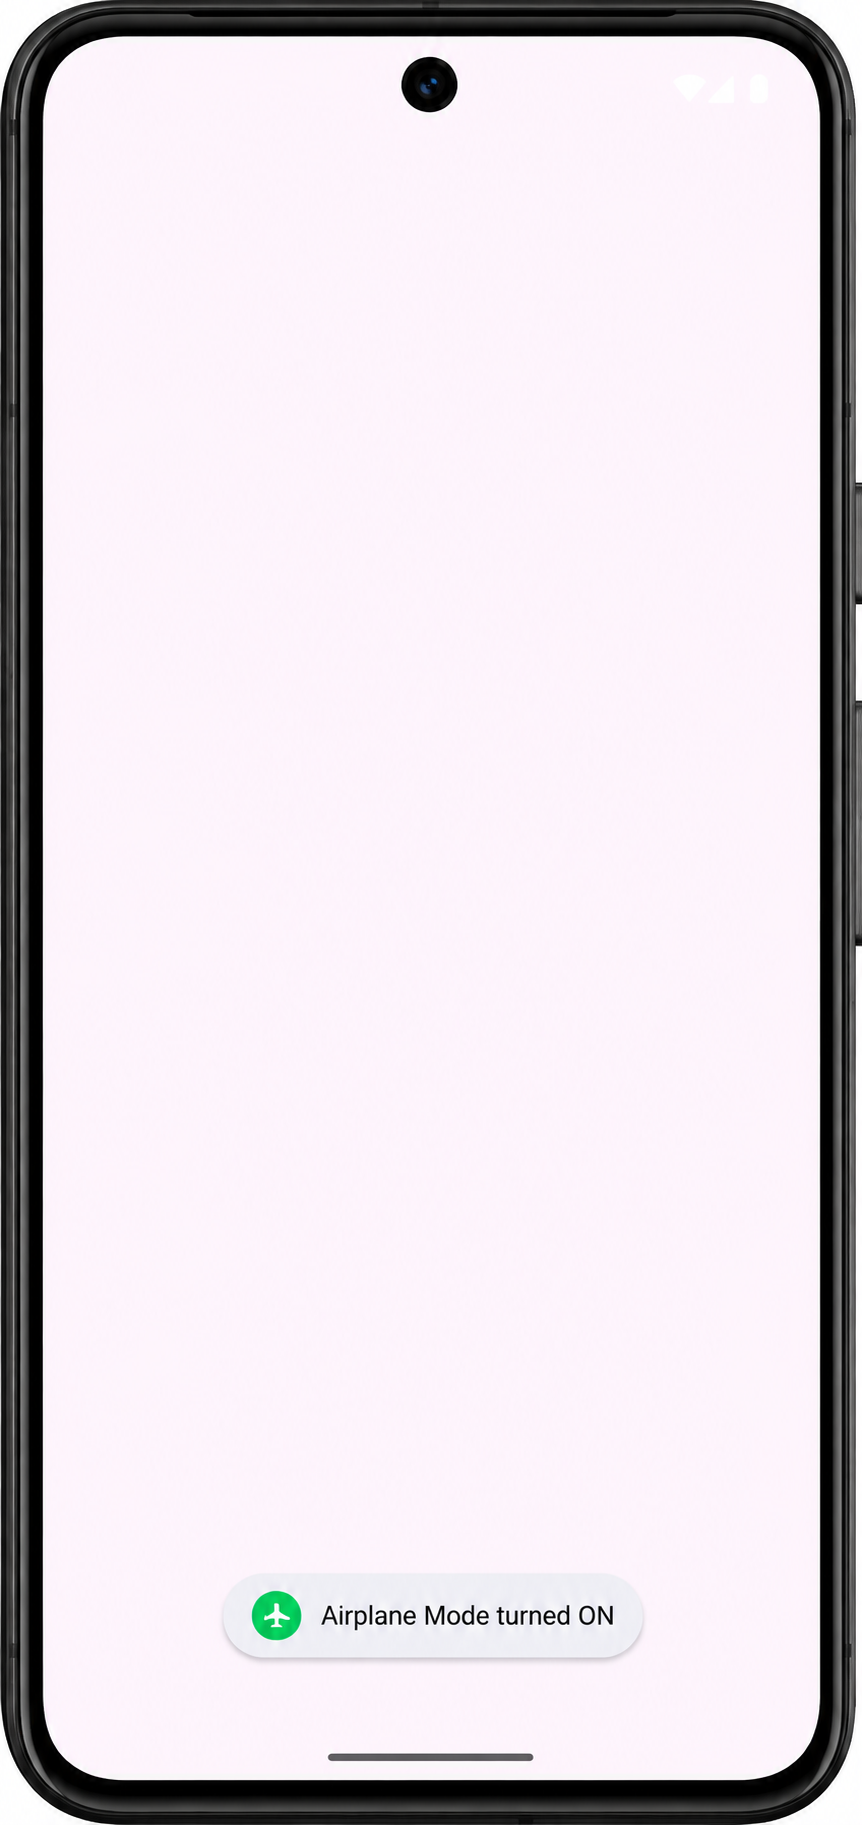
\includegraphics[width=0.45\textwidth]{Output_Screenshots/19.png} \end{center} \\
\end{longtable}
\endgroup

\end{document}
